% !TEX program = lualatex
% !TEX encoding = UTF-8 unicode
\documentclass{book}
\usepackage{graphicx} % Required for inserting images
\usepackage{mdframed}


\usepackage{style}
\usepackage{circuitikz}
\usetikzlibrary{tikzmark}
\usepackage{tikz}
\usepackage{circuitikz}

% \newtcbox{\inlinecode}{on line,
%   box align=base,
%   colback=gray!20,
%   colframe=gray!50,
%   boxrule=0pt,
%   arc=1pt,
%   top=0.5pt,
%   bottom=0.5pt,
%   left=2pt,
%   right=2pt,
%   fontupper=\ttfamily\small
% }
% Define a custom style for x86-64 Assembly
\lstdefinelanguage[x64]{Assembler}%
  [x86masm]{Assembler}% base language
  {morekeywords=[1]{rax, rbx, rcx, rdx, rsi, rdi, rsp, rbp,
                    r8, r9, r10, r11, r12, r13, r14, r15,
                    eax, ebx, ecx, edx, esi, edi, esp, ebp},
   morekeywords=[2]{mov, push, pop, call, ret, jmp, je, jne, cmp, test,
                    add, sub, imul, idiv, xor, or, and, lea, inc, dec}}

% Custom style
\lstdefinestyle{asmstyle}{
    language=[x64]Assembler,
    basicstyle=\ttfamily\footnotesize,
    keywordstyle=[1]\color{blue},
    keywordstyle=[2]\color{purple}\bfseries,
    commentstyle=\color{gray}\itshape,
    morecomment=[l]{;},
    showstringspaces=false,
    columns=fullflexible,
    frame=single,
    captionpos=b
}

% Define a custom style for x86-64 Assembly
\lstdefinelanguage[x64]{Assembler}%
  [x86masm]{Assembler}% base language
  {morekeywords=[1]{rax, rbx, rcx, rdx, rsi, rdi, rsp, rbp,
                    r8, r9, r10, r11, r12, r13, r14, r15,
                    eax, ebx, ecx, edx, esi, edi, esp, ebp},
   morekeywords=[2]{mov, push, pop, call, ret, jmp, je, jne, cmp, test,
                    add, sub, imul, idiv, xor, or, and, lea, inc, dec}}

% Custom style
\lstdefinestyle{asmstyle}{
    language=[x64]Assembler,
    basicstyle=\ttfamily\footnotesize,
    keywordstyle=[1]\color{blue},
    keywordstyle=[2]\color{purple}\bfseries,
    commentstyle=\color{gray}\itshape,
    morecomment=[l]{;},
    showstringspaces=false,
    columns=fullflexible,
    frame=single,
    captionpos=b
}
\newtcbox{\inlinecode}{
    on line,
    boxsep=1pt,
    left=2pt,
    right=2pt,
    top=1pt,
    bottom=1pt,
    colback=gray!20,      % background (Markdown-like)
    colframe=gray!20,     % same color as background (no visible border)
    boxrule=0pt,
    arc=2pt,              % rounded corners
    box align=base,
    fontupper=\ttfamily
}
\let\oldtexttt\texttt
\renewcommand{\texttt}[1]{\inlinecode{#1}}

\lstdefinelanguage[RISC-V]{Assembler}
{
  alsoletter={.}, % allow dots in keywords
  alsodigit={0x}, % hex numbers are numbers too!
  morekeywords=[1]{ % instructions
    lb, lh, lw, lbu, lhu, li,
    sb, sh, sw,
    sll, slli, srl, srli, sra, srai,
    add, addi, sub, lui, auipc,
    xor, xori, or, ori, and, andi,
    slt, slti, sltu, sltiu,
    beq, bne, blt, bge, bltu, bgeu,
    j, jr, jal, jalr, ret,
    scall, break, nop
  },
  morekeywords=[2]{ % sections of our code and other directives
    .align, .ascii, .asciiz, .byte, .data, .double, .extern,
    .float, .globl, .half, .kdata, .ktext, .set, .space, .text, .word
  },
  morekeywords=[3]{ % registers
    zero, ra, sp, gp, tp, s0, fp,
    t0, t1, t2, t3, t4, t5, t6,
    s1, s2, s3, s4, s5, s6, s7, s8, s9, s10, s11,
    a0, a1, a2, a3, a4, a5, a6, a7,
    ft0, ft1, ft2, ft3, ft4, ft5, ft6, ft7,
    fs0, fs1, fs2, fs3, fs4, fs5, fs6, fs7, fs8, fs9, fs10, fs11,
    fa0, fa1, fa2, fa3, fa4, fa5, fa6, fa7
  },
  morecomment=[l]{;},   % mark ; as line comment start
  morecomment=[l]{\#},  % as well as # (even though it is unconventional)
  morestring=[b]",      % mark " as string start/end
  morestring=[b]'       % also mark ' as string start/end
}

\lstset{
  backgroundcolor=\color{gray!10},
  basicstyle=\ttfamily\small,
  keywordstyle=\color{blue},
  commentstyle=\color{green!60!black},
  stringstyle=\color{orange},
  showstringspaces=false,
  breaklines=true,
  frame=single,
}




\title{Computer Architecture \\ Prof. Paolo Ienne}
\author{Arthur Herbette}
\date{October 2025}

\begin{document}

\maketitle

\newpage
\tableofcontents
\newpage
\chapter*{Introduction}
This document is the note I have written during and outside of the course, all the information here is directly taken from the course, slides, etc... However mistake can happen, if you see some mistake or see something that is not clear, feel free to ping an issue on the github \href{https://github.com/Arthur926564/LectureNotes}{LectureNotes}, or email/telegram me.\\
\textbf{Disclaimer} in this course, when we say \textit{high-level language} we mean a language that is compiled/interpreted for instance: \texttt{c} is a high-level language here.
\subsection{Content of the course}
The course is divided into three parts:
\begin{itemize}
	\item \textbf{Part I: Processors and ISA}  \\ What is a processor? How can we design one? How do programs look like when they are executed? 
	\item \textbf{Part II: I/Os and Exceptions} \\ What is arounf a processor to make a full computer? How the processor exchanges information with the rest of the world? 
	\item \textbf{Part III: Memory Hierarchy} \\ Processors are fast and memory is slow -how can one combine the two? How can one protext the data users in memory
	\item \textbf{Parti IV: Instruction-Level Parallelism} \\ What makes a good processor? How real processors achieve ever increasing performances? 
	\item \textbf{Part V: Multiprocessors} \\ What are the basic challeng of connecting many processors together? What changes from a single processor system? 
	\item \textbf{Parti VI: Rudiments of Hardware Secrurity} \\ How can a hacker exploit what we have built in the previous parts to attack a system? How physics helps jeopardizing security?
\end{itemize}
\subsubsection{Literature}
The course will have two books for the literature which are the same as the one for fds :
\begin{enumerate}
    \item Digital Design: Principles and Practices John F. Wakerly 
    \item Computer organization and design: The hardware software interface David A. Patterson, John L. Hennessy
\end{enumerate}

\part{Midterm}
\chapter{Processors and instruction set architecture}

\section{Instruction set architecture}
The goal for the beggining of this course is to go from "high-level" perspective to the bottom of the iceberg. First let us look at a piece of code (\texttt{c}):

\begin{lstlisting}[language=c]
int data = 0x00123456;
int result = 0;
int mask = 1;
int count = 0;
int temp = 0;
int limit = 32;
do{
   temp = data & mask;
   result = result + temp;
   data = data >> 1;
   count = count + 1;
} while (count != limite);
\end{lstlisting}
Here we can see that we have variable with expressive names (that we can choose). each variable has a type, the computation we are doing \texttt{result + temp} looks like a mathematic formula, the control flow we are using is very intuitive.\\
In the case of those high-level language, we have an "unlimited" number of variables which supports any type.\\
If we wanted to convert this code into Assembly code we would have this:
\begin{lstlisting}[language={[RISC-V]Assembler}]
    li x1, 0x00123456
	li x2, 0 
	li x3, 1 
	li x4, 0 
	li x5, 0 
	li x6, 32
loop:
	and x5, x1, x3
	add x2, x2, x5 
	srli x1, x1, 1 
	addi x4, x4, 1 
	bne x4, x6, loop
\end{lstlisting}
As we can see we have a much more rigid format: we really have a sequence of numbered instructions that is executed line by line. For each instructions, we have an \textit{opcode}  that defines the effect of the instruction. Each \textit{variable} has a fixed name and we only have one form of control flow. The question to ask is why did we do that?\\ The answer of thie question lays is in the architecture of the processor:
\begin{center}
\includegraphics[scale=0.6]{screenshots/2025-10-11_1.png}
\end{center}
how it works: the processor fetch the instruction at the address of the program counter (PC) and launch it to the control logic
\begin{center}
\includegraphics[scale=0.6]{screenshots/2025-10-11_2.png}
\end{center}
After that the instruction has been fetch, it is processed in the Control logic and then read/write etc... into the register file, and give the information (the opcode) to the ALU for it to know which operation to perform.
\begin{center}
\includegraphics[scale=0.2]{screenshots/2025-10-11_3.png}
\end{center}
\subsubsection{The five classic components of a computer}
For an every day computer you need four other components other than the control components, you need to have a memory to store data (bigger than 32 word registers), you need to take input from the outside worlds (Internet, bluetooth, a keyboard, mouse ...) and also output something to the outside word.  On top of that, you need all of that to communicate $\implies$ you need a data path.
\begin{center}
\includegraphics[scale=0.3]{screenshots/2025-10-11_4.png}
\end{center}
Okay, we have memory, we have input output and a place to compute everything, but what do we need to compute? Where is the program that is being executed? At the moment we have a place for the data but not for our program so how do we do it? \\ 
We store the program in the same memory than the one for the data. This is called a \textit{Unified Architecture} (On the other hand, an architecture that have two seperates memory, one for the instruction and one for the data is called a \textit{Harvard Architecture}). This is a \textbf{Key concept to computer science}, our instruction (therefore program) are represented as numbers (juste like data).
\begin{center}
\includegraphics[scale=0.3]{screenshots/2025-10-11_5.png}
\end{center}
   Now a good question to have is: how to decode and encode those instructions and in the mean time, also what makes a good encoding? \\
A good encoding would be one that allows us two minimize the ressource in hardware and also is the fastest. This is where \texttt{RISC-V} comes in the play!! \texttt{RISC-V} is an instruction set architecture as like many others for instance x86, x64 for the most famous and used one.\\ 
The difference between assembly language and high-level language is in the "\textit{translation}", for the assembly language, we use an \important{assembler}, for a high-level language (a compiled one), we use a \important{compiler}:
\begin{itemize}
	\item Assembler can easily translate from code to binary code (this is what the instruction set tells us to do). All we need to do is the look up in the table and translate 
	\item A compiler on the other hand cannot look up in a table, it has to translate the code into Assembly code to be translated, but compiled the code into Assembly is a very hard thing to do, you have to find the best way or at least, try to find the best way to say the same thing but in assembly.
\end{itemize}




	\section{Instruction set architecture: Branches, Function and stack}
	The main goal that ISA does is to put a \textbf{Contract} between the hardware and the software: If you are an hardware person, all you care about is the make your processor the fastest on the ISA. If you are a software person, you don't need to worry about the hardware behind anything, you only care about the software that you are building. This ISA gives a level of abstraction which makes it easier to develop better software/hardware.
	\begin{center}
	\includegraphics[scale=0.3]{screenshots/2025-10-11_6.png}
	\end{center}
	As we have seen in cs-173, arithmetic and logic operation are quite easy to understand and use in RISC-V. But here are some facts to know about them:
	\begin{itemize}
		\item Immediate constant takes at maximum 12 bits. The reason behind this is that the immediate part of the instruction is directly stored in the instruction, this means that there are 12 bits of the instruction that are reserved for the immediate part. Imagine having for instance a 30 bits immediate, then you would only have 2 bits for: the opcode, result register, input register ... 
		\item A way to go around this is to use the \texttt{.equ, num} and then to use \texttt{lui} directly on \texttt{num}. (this is possible because the assembler will directly translate the one line instruction into a three lines instruction). 
		\item Register \texttt{x0}, this register is \textbf{always} zero (by definition), you can write anything to this resgister, the value in it will always be zero. This can be useful  in a lot of case, it happens quite often that we need a zero in a instruction and the only way to do so would have been to \texttt{li} a register to 0 and then calling the instruction. Therefore, the \texttt{x0} register allows us to save instructions
	\end{itemize}

	\subsubsection{An if-then-else}
	To be able to do an if and else cause will need some branches, for instance if we wanted to translate the code:
	\begin{lstlisting}[language=c]
	if (x5 == 72) {
	   x6 = x6 + 1
	} else {
	   x6 = x6 - 1
	}
	...
	\end{lstlisting}
	Into RISC-V: it would look like this:
	\begin{lstlisting}[language={[RISC-V]Assembler}]
	.text 
		li x7, 72
		beq x5, x7, then_clause
	else_clause:
		addi x6, x6, -1 
		j end_if
	then_clause:
		addi x6, x6, 1 
	end_if:
		...
	\end{lstlisting}
	As you can see jump and branch are really similar however, there is a universal distinction between them:
	\begin{itemize}
		\item Jumps $\to $ \important{unconditional} control transfer instructions
		\item Branch $\to $ \important{conditional} control transfer instructions
	\end{itemize}
	However this is not the case for every assembly languages, for instance in x86, everything is defined as a jump.
	\subsubsection{A Do-while loop}
	\begin{center}
		A do while loop in c
	\end{center}

	\begin{lstlisting}[language=c]
	do {
	   x5 = x5 >> 1 
	   x6 = x6 + 1 
	} while (x5 != 0);
	...
	\end{lstlisting}

	\begin{center}
		A do while loop in risc-v
	\end{center}
	\begin{lstlisting}[language={[RISC-V]Assembler}]
	.text
	loop:
		srli x5, x5, 1 
		addi x6, x6, 1 
		bnez x5, loop 
	...
	\end{lstlisting}
	\subsection{Functios}
	In our high-level code, we usually use function to organized our code (Scala...) (those function can also be called methods, procedure dependeing of the context).\\ 
	What we would like is also to have function in assembly so that we don't have to write the same code always. What a function would look like is:
	\begin{enumerate}
		\item Place arguments where the called function can access them 
		\item jump to the function 
		\item Acquire storage resources the function needs 
		\item Perform the desired task of the function 
		\item Communicate the result value back to the calling program 
		\item realease any local storage resources 
		\item Return control to the calling program
	\end{enumerate}
	That sound pretty hard to do so let's do it step by step. First, the second and seven steps (I know).\\
	What we need is to jump to the function and the return. This is fairly easy to do, all we need is to call the jump instruction. For instance, let's call the function two times. This  would looks like this
	\begin{lstlisting}[language={[RISC-V]Assembler}]
	sqrt:
		...
		j back
	\end{lstlisting}
	And the main would look like this:
	\begin{lstlisting}[language={[RISC-V]Assembler}]
	main: 
		...
		j sqrt 
	back:
		...
		j sqrt 
	back2:
		...
	\end{lstlisting}
	However, isn't there an issue? what would happen if we tried to run this code?\\
	The answer is that this would lead to an infinite loop. the \texttt{sqrt} function doesn't know about the fact that there are more than one back.
	The solution to this problem is to:\\
	when you called the function, you store the current PC $+ 4$  (to go to  the next line) to a register (for instance \texttt{x1}). You then, call the function, do the computation there \textbf{and then} you rejump to the address store in the register \texttt{x1}.

	\begin{parag}{Jump and link}
		


	There is instruction that allows us to do this, those instruction are called jamp and link \texttt{jal}, and the other one is called jump to the address specified in a register \texttt{jr}, however we said before that we only use \texttt{x1} for the return address so why don't we make an instruction that directly jump to this address: \texttt{ret} (which stands for return I think).\\
	However what we have to be careful with here is that the \texttt{x1} register is not preserved accorss the call (this is not something that is known for now but let me explain it shortly). What we will want to do is the call function inside function (have call inside call inside call etc ...) however every time we make a call to a function, the x1 register will be overwritten: every time you jump and link, you store in the return address register the pc $+ 4$. However this is not currently a problem, we will solve it later.
\paragraph{Acquire storage ressource the function needs}
There is a lot of way to do this. The first way to do so is to juste allocate like 10 registers to the current function and the rest to the function that is called. for instance
if we have this code:
\begin{lstlisting}[language={[RISC-V]Assembler}]
main:
	...
	jal sqrt 
	... 

	... 
	jal sqrt
	...
ret 

sqrt: 
	...

	add x5, x7, x8 
	jal round 
	sub x6, x6, x5 
	...
	ret

round:
	...
	addi x10, x11, 3 
	...

	ret
\end{lstlisting}
You see that the round procedure only use the register \texttt{x10} to \texttt{x15}. and that sqrt the one from 2 to 9. We can clearly see that this is not scalable, so we need another solution.
\end{parag}
\subsection{The stack}
The \important{stack} is the solution!! Fisrt what is the stack:\\
\begin{definition}
$ $\\
\begin{itemize}
    \item The stack is a empty region in the memory 
    \item We use the register \texttt{x2} (also called \texttt{sp}) to store the address of the end of the used region
    \item If we are using all variables and we still want to make a call to a function, we need to store in the stack our variable before calling the function and then restore our variable from the stack.
\end{itemize}
\end{definition}
The complexity of this is to understand the order of what is needed to be stored or not. For instance if you have a function that is being called from above. We have to be sure that we don't overwrite the values from the function that is above. to do so, we store the value in the stack and restore them afterward. (only the register that we are changing). to do so we have to dynamically allocate more space in the stack.\\ 
Here is an example:
\begin{lstlisting}[language={[RISC-V]Assembler}]
	...
	addi sp, sp, -8 
	sw x8, 0(sp)
	sw x9, 4(sp)
	...
	#we have here free use of x8 and x9
	...
	lw x9, 4(sp)
	lw x8, 0(sp)
	addi sp, sp, 8
\end{lstlisting}
However, do we need to store all the register? how do we return something, how do we pass arguements to a function. To do so we agree to use some register as arguement, return register, other for return address, stack pointer, temporaries, saved... I strongly advise to go read the RV32i Reference Card.\\
So what do we still need? we are currently able to jump to function, return from the function, acquire storage resources, perform the desired stack of the function, All we need is the arguement and return values.
To do so is very simple, as I said before we can:
\begin{itemize}
    \item Use some particular registers, both for the \important{arguments} and for the return \important{result}.
    \item We can do it ad-hoc ...
		\begin{itemize}
		    \item \texttt{sqrt} gets the arguement in \texttt{x5} and returns the result in \texttt{x6}
		\end{itemize}
	\item Or we can have some convention
		\begin{itemize}
		    \item All function pass arguements in register \texttt{x10} to \texttt{x17} and return the result in \texttt{x10}
		\end{itemize}
		\item Can this be insufficient? \important{More arguments} than allocated registers? What if we have 10 arguements
\end{itemize}

\paragraph{Option 2}
If we don't have enough registers, we can just put them in the task right? we know that the stack is unlimited (in theory), all we would need is to do more work (allocate space, storing, loading etc ...)\\
To do so we can use another register: \texttt{fp} or \texttt{x8} in risc-v which point to the same location as sp on entry. \\
This make the code more readable because:
\begin{itemize}
	\item \texttt{sp} changes inside the function and so do relative offsets 
	\item offests with respect to the \texttt{fp} are \important{fixed}
\end{itemize}
The use of the fp register is \important{optional} and even varies among users and compilers. (I personnaly didn't use it during lab 1, I only used the registers that are reserved).\\
\begin{center}
\includegraphics[scale=0.3]{screenshots/2025-10-11_7.png}
\end{center}


















\section{Memory and Addressing Modes}
\subsection{Memory}
Memory is an incredibly important component of a computing system:
\begin{itemize}
    \item We store our \important{programs} in it 
    \item We store our \important{data} in it 
	\item It is often through memory that we will \important{receive data and send out data}
\end{itemize}
	Memory is a reccurent ropic in this course, we have already seen it with the stack however the type of the memory is also an important topic:
	\begin{itemize}
		\item Memory can be \important{very slow} $\implies $ Caches 
		\item Memory is \textit{finite} (relatively small) $\implies $ Virtual memory 
		\item Memory can make an \important{ISA too complex} $\implies $ pipelining
	\end{itemize}
	\paragraph{Types of memory}
	There is a lot of different technologies for memory:
	\begin{itemize}
		\item SRAM, DRAM, EPROM, Flash, etc.
\end{itemize}
Each of those has a variations in \important{capabilities} therefore also in how we use them, memory change by:
\begin{itemize}
	\item Capacity, density 
	\item Speed 
	\item Writable, permanent, reprogrammable
\end{itemize}
\begin{center}
\includegraphics[scale=0.4]{screenshots/2025-10-11_8.png}
\end{center}
We have here all the type of memory that can be used, What we use when we program are Random access memory, this means that the memory can be accessed with an address. In the tree of random access memory we have:
\begin{center}
\includegraphics[scale=0.4]{screenshots/2025-10-11_9.png}
\end{center}
The basic structure behind those memory are DFF, (D flip flop). which are stacked one on another in a $n$ times 4 grid. Each flip flop looks like this:
\paragraph{SRAM}
SRAM stands for \important{static random access memory}. It sores data with flips flops which makes it faster than DRAM (which we will see later) but more expensive. We use it for CPU caches and for the register file
\begin{center}
\includegraphics[scale=0.3]{screenshots/2025-10-11_10.png}
\end{center}
So here we have to make a difference between the boolean system and the electrical components. The circuit on the left is a desastre in term of electrical components it has approximatevely 20 transistors which makes it \important{slower} \textbf{and} \important{costlier}. The real way to do SRAM is with the right circuit. However this looks bad, normally it is forbidden to have a closed loop in a circuit! We are forbidden to have a loop in our circuit without a flip flop in it, you cannot have a loop inside a combinational circuit. So this is a big special thing for us however, this "works", it is compatible there is no issue in the circuit. The issue we have is that:\\
Imagine putting a one on the left or right part of the circuit $\implies$ the value cannot be changed, it is stucked there for ever. This looks really good because one \textbf{NOT} gate costs us only two transistors so the memory (loop) costs us only 4 transistors. But we still need to write and read from the memory, to do so we had the two transistors (see on the image) which also us to let the memory live on its own (when the transistors are open) \textbf{or} to be connected to the world. \\
If I want to see what is on the memory I put one in the word line (WL) and I will get the value on the bit line.\\
The question now is how to write? As said earlier, now we have a signal that is stored in there but it is stored for infinity.\\
The only way to write is to "\textit{shout louder than the current signal}".  Imagine we currently have a 1 as the output of the latch and I want to put a 0. If I shout 0 louder than the 1 while connected, it will have a short circuit... and this is bad. \textbf{However} what is going on in fact is the upper not gate will have two inputs, a \textbf{loud} 0 and a quiet 1, the not fate will then take the loudest one thus 0.\\
And now it will take a really short time to the latch to adapt itself to the new value, the short circuit here take the times two the 0 to go trhough two not gates. and then it agrees.\\

On the other hand we have DRAM:
\paragraph{DRAM}
\begin{itemize}
    \item  Dynamic RAMs are the densest (and thus cheapest) form of random access semiconductor memory 
    \item DRAMs store \important{information as charge in small capacitors} part of the memory cell 
    \item First parented in 1968 by Robert Dennard, scaled amazingly over decades and was somehow an important ingredient of the progress of computing systems.
    \item charges \important{leaks off} the capacitors due to parasitic resistance $\implies $ every DRAM cell needs a \important{periodic refresh} (e.g. every \~60ms) lest it forgets information.
\end{itemize}
So imagine, if we don't go in each cell every 60ms then we lose the information, but we have other things to do? So how do we do it? - we have someone else refresh them for us. The memory controller is reponsible for refreshing the contents of the DRAM instead of the CPU.
\begin{center}
\includegraphics[scale=0.3]{screenshots/2025-10-12.png}
\end{center}
The goal after this is to access those memory celle based on the address we input. The \textit{ideal} way to do so, would be to have one \textbf{big} decoder that treats the adress and directly output the information in the memory celle like this:
\begin{center}
\includegraphics[scale=0.2]{screenshots/2025-10-12_1.png}
\end{center}
However life is not always that easy, and there is a lot of way to get the memory celle based on the address, here are some example:
\begin{center}
\includegraphics[scale=0.4]{screenshots/2025-10-12_2.png}
\end{center}
Here we have 3 ways to do so:
\begin{itemize}
    \item On the left, We have the same way as the \textit{ideal} decoder with one byte per row 
    \item However we can also split up into a grid with more than one \textbf{big} multiplexer. This implies that there will be multiple word by row and that the bytes are not necesserly ordered.
\end{itemize}
The best physical way to create a Random access memory is in a square to minimize parasitic capacitance of BL (bit line) and WL (word line). We want to having it into the most squared possible form because:
\begin{itemize}
	\item When a word line is activated (row), the bit line carries the data (bit) stored in the selected memory cell to the output circuitry (like a multiplexer or sense amplifier).
	\item Activating a word line selects all the bits (across bit lines) in that row — this is your selected "word."
\end{itemize}
Therefore by having the smallest length, we get shorter lines $\implies $ lower parasitic capacitance $\implies$ faster access, lower power, and more reliable operation.
\begin{center}
\includegraphics[scale=0.3]{screenshots/2025-10-12_3.png}
\end{center}

\begin{framedremark}

Every time we are looking for a memory cell, we need to charge all row and then all column, the goal here is to minimize the number $x =r + c$ by a fixed area $A$ (where $A$ is the number of cell):\\
We have that
\begin{align*} A = rc \\
				\frac{A}{c} = r
\end{align*}
Which implies that $x = \frac{A}{c} + c$, we are minimizing  ($x' = 0$) this:
\begin{align*} 
	x' = -\frac{A}{c^2} + 1 \\
	\frac{A}{c^2} = 1 \\
	c^2 =  A \implies c = \sqrt{A}
\end{align*}
And because we know that $A =  rc \implies r =  c =  \sqrt{A}$ which is a square.

\end{framedremark}
\paragraph{Static RAM typical interface}
This is the typical synchronous SRAM that we have already seen before:
\begin{center}
\includegraphics[scale=0.2]{screenshots/2025-10-12_4.png}
\end{center}
However we don't always has to be synchronous, we can also be asynchronous for a Read cycle which works like this:
\begin{parag}{Asynchronous read cycle}
    

\begin{itemize}
    \item Enable the memory $\to$ assert the address $\to $ wait for the data 
		\begin{itemize}
		    \item Data out is available after a combinational delay $T_{acc} = $ Access Time 
		\end{itemize}
		\item Maximum frequency is limited by the minimum $T_{cyc}$ (time for a cycle, time for us to be able to change the address)
\end{itemize}

\begin{center}
\includegraphics[scale=0.25]{screenshots/2025-10-12_6.png}
\end{center}

\end{parag}
\begin{parag}{synchronous SRAM Read cycle}
    

Here this is the other way around, we always wait a rising edge of the clock to do anything. Everything here is working like a flip flop:
\begin{itemize}
    \item Everything is relative to the clock signal
    \item Latency is the number of cycles between the address asserted and data available
		\begin{itemize}
			\item Often one as in this diagram but in some cases (large memories) more
		\end{itemize}
\end{itemize}


\begin{center}
\includegraphics[scale=0.25]{screenshots/2025-10-12_7.png}
\end{center}
\end{parag}
\subsubsection{Load and store instrucitons}
Now that we have seen how it works, we want to see how to implement a load from the memory into the register file. For instance the following intrsuction:
\begin{lstlisting}[language={[RISC-V]Assembler}]
lw x5, (123456)
\end{lstlisting}
This is not a RISC-V instruction but bear with us. (I am not sure that's a saying...)


\begin{center}
\includegraphics[scale=0.3]{screenshots/2025-10-12_8.png}
\end{center}
What we have changed here is the left part now instead of having a loop like $\text{ALU} \to \text{Register file} \to \text{ALU}$ we break it at the first "$\to$" and add a multiplexer there to be able to interact with the memory. \\

For the store instruction, instead of using the \texttt{MemDataOut} path, we use the \texttt{MemDataIn}.\\
The main diffrence is this:
\begin{center}
    


\begin{tikzpicture}[
    block/.style = {draw, minimum width=2.4cm, minimum height=1cm, align=center},
    arrow/.style = {thick, -{Latex}},
    node distance=1.8cm and 1.8cm
]

%% LOAD PATH

\node[block] (regfileL) {Register File\\(base)};
\node[block, right=of regfileL] (aluL) {ALU\\(base + offset)};
\node[block, right=of aluL] (memL) {Memory};
\node[block, right=of memL] (outregL) {Register File\\(destination)};

\draw[arrow] (regfileL) -- (aluL);
\draw[arrow] (aluL) -- (memL);
\draw[arrow] (memL) -- node[above]{\scriptsize{MemDataOut}} (outregL);

\node[above=0.5cm of aluL] {Load Instruction};

%% STORE PATH

\node[block, below=2.5cm of regfileL] (regfileS1) {Register File\\(base)};
\node[block, right=of regfileS1] (aluS) {ALU\\(base + offset)};
\node[block, right=of aluS] (memS) {Memory};

\node[block, below=1.5cm of aluS] (regfileS2) {Register File\\(value)};
\draw[arrow] (regfileS1) -- (aluS);
\draw[arrow] (aluS) -- (memS);
\draw[arrow] (regfileS2) -- node[right]{MemDataIn} (memS);

\node[above=0.5cm of aluS] {Store Instruction};

\end{tikzpicture}
\end{center}
\begin{framedremark}
	I had some trouble understand how does the value just pop, but if I understand it right, the register value is stored from the register file into \texttt{B} here. We use the \texttt{A} port as a address base. This is how it works:
\begin{enumerate}
    \item IF, Fetch instruction ( \texttt{sw x2, 8(x1)})
    \item ID, Read \texttt{x1} and \texttt{x2} from register file 
    \item EX, ALU compute \texttt{x1 + 8} (address) 
    \item MEM, Store \texttt{x2} to memory at computed address 
    \item WB, Nothing (no register to write for store)
\end{enumerate}
\end{framedremark}

\paragraph{Why RISC-V instructions are so simple?}%
\label{par:Why RISC-V instructions are so simple?}

\begin{framedremark}
Here are some example of some instruction that would look correct in RISC-V but is not (for addition):
\begin{itemize}
    \item Based or Indexed
		\begin{lstlisting}[language={[RISC-V]Assembler}]
	add x0, x1, i5(x2)		#x0 = x1 + mem[x2 + i5]
		\end{lstlisting}
	\item Auto-increment or -decrement
		\begin{lstlisting}[language={[RISC-V]Assembler}]
	add x0, x1, (x2+) 		#x0 = x1 + mem[x2]
		\end{lstlisting}
	\item PC-relative
		\begin{lstlisting}[language={[RISC-V]Assembler}]
	add x0, x1, 123(pc)		#x0 = x1 + mem[pc + 123]
		\end{lstlisting}
\end{itemize}
However those instruciton \important{does not exist} in RISC-V.\\
RISC-V is designed to have  two world: one for accessing memory, and one for the logic/arithmetic etc. We cannot mix them together.\\
However in x86/x64 we can do this:
\begin{lstlisting}[language={[x64]Assembler}]
	ADD DWORD PTR [EBX + ESI*4 + 16], EAX
\end{lstlisting}
This means:
\begin{itemize}
    \item The \texttt{DWORD} means double word which means that we are working on 64 bits number.
	\item The \texttt{ADD} that has only two operand, the reason why, is that the goal of x86 in 1979 was to be the most compact possible, at that time the memory was limited and to be able to write program you had to be careful of the size of the program that you are writing. So they added the constraints that the output of the instruction is stored in the first operand. \\ this means we take something in the memory at \texttt{[EBX + ESI*4 + 16]}, add it with \texttt{EAX} and then store it in \texttt{[EBX + ESI*4 + 16]}. 
\end{itemize}
	 this feels pretty slow and pretty confusing, just try to map this into the CPU we created before, this would look like this:
		\begin{center}
		\includegraphics[scale=0.2]{screenshots/2025-10-12_9.png}
		\end{center}
We would need to go like four times to the ALU, the fact is that \important{this is possible} however it makes it hard to optimize the processor.
\end{framedremark}
The question behind all this is how does intel can still be as famous as they are now with instruction that looks like this and that cannot really be optimized? There is still the majority of the processor to this day that are intel processor (even if amd is better...), we will see this in a couples of weeks.
\subsubsection{Byte addressed memory}

Almost all ISA today are use byte addressed memory. byte are quite important, disks are organized in bytes, network packets are bytes, \important{ascii} are byte. A lot of data are represented as byte so using an word addressed memory wouldn't be very efficient here, we would either loose a lot of time looking for the right byte, or loosing a lot of space by putting byte in word address (losing the three other bytes).\\
The solution is to no change the way memory is placed \textbf{but} \important{changing the label}.
\begin{center}
\includegraphics[scale=0.3]{screenshots/2025-10-12_10.png}
\end{center}
\paragraph{Loading a word (\texttt{lw}) and Instruction}%
For instance, if we are interested in word, we cannot look for the word at address 3981, this would'nt be a word.
\begin{center}
\includegraphics[scale=0.25]{screenshots/2025-10-12_11.png}
\end{center}
As said before when loading a word, it has to be a multiple of 4 so we only care about the 30 most significant bits. The two least significant bits is checked wether there are zero or not and if there are not zero, we would like to \important{throw an exception} which we will see how in a couple of weeks.

\paragraph{Loading bytes (\texttt{lb})}
\label{par:Loadingbytes}

Here what we are doing is the same as what we did before, we are looking for a word (which is the 30 first bits), and then in the word we choose which 8 bits we wants, this would look like this:
\begin{center}
\includegraphics[scale=0.25]{screenshots/2025-10-12_12.png}
\end{center}

Remember when we changed the shape of the memory, how we choose which bit to take; we are doing  the \important{same} here too. The difference is that this part is only in the processor, circuit wise this change nothing.\\
What is good here is that by just adding a multiplexer we can add a lot of instruction in the ISA.

\section{Arrays and data structures}
Data structures is one of the main concept in computer science, even in this course we have already talk about it (the stack).\\
\begin{parag}{Arrays in high-level languages}
	\begin{lstlisting}[language=Scala]
val myData: Array[Short] = Array(10407, -16533, -22715, 123133, 12512)
    \end{lstlisting}
Here we have a sequence of number that are indexed, the question however is how do we store them?\\
We have a lot of ways to do so (three), we can:\\
have a pointer to the first element, and the having the other element following this one. With this method the issue is when does the array stops? here's three example of how to store arrays:
\begin{enumerate}
    \item One way to do so is to put a \textit{null} element at the end of the array so that we know that this is the end of the array.  The definition of string are in fact an array of char with the 0 char at the end.
	\item A whole other way is to have, at the start of the array the length of the array. You have a pointer at the start of the array which is the length of the array and then you do your computing as usual
	\item Another way with this is just to to do nothing. Having a pointer to the start of the array and then hoping that the programmer knows what he is his doing. \texttt{C} Arrays for instance are built like this.
\end{enumerate}


\end{parag}
\begin{center}
\includegraphics[scale=0.3]{screenshots/2025-10-21.png}
\end{center}
\begin{parag}{Adding Positive elements}
    To add all the positive elements in an array of signed 16-bit integers we would:
	\begin{itemize}
	    \item At call time \textrightarrow \texttt{a0} points to the array (and, in type 3, \texttt{a1} is the length)
	    \item At return time \textrightarrow \texttt{a0} contain the result
	\end{itemize}
	The result for the type 3 (written in \texttt{c}):
	\begin{lstlisting}[language=c]
short add_positive(short myData[], int N) {
	short  sum = 0;
	for (int i = 0; i < N; i++) {
		if (myData[i] > 0) {
			sum += myData[i];
		}
	}
	return sum;
}
	\end{lstlisting}
\end{parag}
\begin{parag}{Adding positive elements (Type 1)}
    For the first type let us write the code in RISC-V:
	\begin{lstlisting}[language={[RISC-V]Assembler}]
add_positive:
	li t0, 0  #t0 will hold the sum (initialized to 0)

next_short:
	lh t1, 0(a0) # Load short (half-word) at address a0 into t1
	beqz t1, end  # If t1 is 0 (null short) we are done
	bltz t1, negative  # if t1 is negative ignore
	add t0, t0, t1  #Add t1 to the sum (t0)

negative:
	addi a0, a0, 2  # move array pointer (a0) by sizeof(short) to the next element
	j next_short  # repeat the loop
end:
	mv a0, t0  # move the sum (t0) into a0 as the return value
	ret # Return the caller
	\end{lstlisting}
	
	
\end{parag}

\begin{parag}{Adding positive element Type 2}
	\begin{lstlisting}[language={[RISC-V]Assembler}]
addi_positive:
	li 01, 0 #t0 will hold the sum (initialized to 0)
	lh t1, 0(a0) # t1 will count the elemetnts to process
	add a0, a0, 2  # Move array pointer (a0) to the first real element

next_short:
	beqz t1, end  # If t1 is 0 (no more elements), we are done
	lh t2, 0(a0) # Load short (half-word) at address a0 into t2
	bltz t2, negative # If t2 is negative, ignore
	add t0, t0 t2  # Add t2 to the sum (t0)

negative:
	addi a0, a0, 2 # Move array pointer (a0) by sizeof(short)
	addi t1, t1, -1 # Decrement the counter of elements to process
	j next_short  # repeat the loop
end:
	mv a0, t0 # Move the sum (t0) into a0 as the return value
	ret # Return to caller
\end{lstlisting}

\end{parag}



\begin{parag}{Adding positive element Type 3}
	\begin{lstlisting}[language={[RISC-V]Assembler}]
addi_positive:
	li 01, 0 #t0 will hold the sum (initialized to 0)
	mv t1, a1 # t1 will count the elemnts to process (a1)

next_short:
	beqz t1, end  # If t1 is 0 (no more elements), we are done
	lh t2, 0(a0) # Load short (half-word) at address a0 into t2
	bltz t2, negative # If t2 is negative, ignore
	add t0, t0 t2  # Add t2 to the sum (t0)

negative:
	addi a0, a0, 2 # Move array pointer (a0) by sizeof(short)
	addi t1, t1, -1 # Decrement the counter of elements to process
	j next_short  # repeat the loop
end:
	mv a0, t0 # Move the sum (t0) into a0 as the return value
	ret # Return to caller
\end{lstlisting}

\end{parag}

\begin{parag}{Adding positive elements (variation on type 3)}
	Let us add positive elements in an array of signed 16-bits integers:
	\begin{itemize}
	    \item At call time \textrightarrow \texttt{a0} points to the arrays and \texttt{a1} is the length of the array
	    \item At return time \textrightarrow \texttt{a0} contains the result
	\end{itemize}
	The way od doing it is to incremented the index of the array:\\
	\begin{lstlisting}[language=c]
int i = 0;
while (i < N) {
	if (myData[i] > 0) {
		...
	}
	i++
}
	\end{lstlisting}
	This is equivalent to:
	\begin{lstlisting}[language=c]
int i;
for (i = 0; i < n; i++) {
	if (myData[i] > 0) {
		...
	}
}
	\end{lstlisting}
	
	Here we see that we have a variable \texttt{i}  which is incremented by one, therefore, the way of doing this if we were to be compiled would be by having a variable that is incremented by 1 in every loop \textbf{then} be multiplied by the size of the data (2 bytes).
	\begin{lstlisting}[language={[RISC-V]Assembler}]
addi_positive:
	li t0, 0 #t0 will hold the sum (initialized to 0)
	mv t1, 0 # t1 will hold the array index

next_index:
	beqz t1, end  # If index >= number of elements , we are done
	slli t2, t1, 1  # t2 = offset of the element as index (t1) * sizeof(short)
	add t2, a0, t2 # Address of the element = myData (a0) + offset(t2)
	lh t3, 0(t2) # load short (half-word) at address a0 into t3
	bltz t3, negative #if t3 is negative, ignore
	add t0, t0, t3 # Add t3, to the sum (t0)

negativ:
	addi t1, t1, 1 #Increment the counter of element to process
	j next_index  # repeat the loop
end:
	mv a0, t0 # Move the sum (t0) into a0 as the return value
	ret # Return to caller
	\end{lstlisting}
	
	\begin{subparag}{Which one is better?}
	    We have now two different way to do the same type (type 3), however which one is faster? this question can be easily answers: \\
		the first one that we have written has less intrustion $\implies$ faster. (this is not always that simple)\\
		But this points out an issue, we need \important{good compiler}, we need a compiler that can translated our code into the \important{fastest assembly code possible}.
	\end{subparag}
\end{parag}


\begin{parag}{Linked list}
    Another way to store data is with a linked list:
	\begin{center}
	\includegraphics[scale=0.3]{screenshots/2025-10-21_1.png}
	\end{center}
	As we can see here this is the same principle as what we did before, we store for each element the current address of the value \important{and} the address of the next value. To  iterate through this list all we have to do is to go to the current value get the value via the address and then take the next iteration with the second address.\\
	What is good about this is that:
	\begin{itemize}
	    \item  Insert element in the array is very easy
	\end{itemize}
	However there is a lot of bad thing here:
	\begin{itemize}
	    \item For each value we have to use 64 bits of addresses which is a lot 
		\item iterate through the list seems nice however are all the instruction truly equal?	
	\end{itemize}
	For  instance imagine we wanted to recreate the same code as the one we wrote for the other arrays:
	\begin{lstlisting}[language={[RISC-V]Assembler}]
add_positive:
	li t0, 0 # t0 will hold the sum
next_element:
	beqz a0, end # If address of next element (a0) is zero, we are done
	lw t1, 0(a0) # Load address of actual data into t1
	lh t1, 0(t1) # Load short (half-word) at address t1 into t1
	bltz t1, negative # if t1 is negative, ignore 
	add t0, t0, t1  #  Add t1 to the sum (t0)

negative:
	lw a0, 4(a0) # Load address of next element into a0
	j next_index
end: 
	mv a0, t0 # Move the sum (t0) into a0 as the return value
	ret # Return to caller
	\end{lstlisting}
	
	As we can see here: this is not much more complex. but is it more efficient?\\
	\important{no}. The instruction of loading and storing are way \important{slower} than the other instruction, the fact that this way of computing leads to a lot more of load makes it way slower.loading byte
\end{parag}







\section{1.e: Instruction Set architecture Arithmetic}
\begin{parag}{Notation}
    \begin{itemize}
        \item Number (represented on a specific no. of digits/bits)
			\begin{align*} A =  A^{\left(n\right)}  =  A^{\left(m\right)}\end{align*}
		\item  Number (in binary or decimal)
			\begin{align*} A = A_{10} =  A_2 = A_{2c} \end{align*}
			\item Individual digits (bits)
				\begin{align*} a_{n-1}, a_{n-2}, \ldots, a_2, a_1, a_0 \end{align*}
				\item Digit string (representation)
					\begin{align*} <a_{n-1}a_{n-2}\cdots a_2 a_1 a_0> \end{align*}
    \end{itemize}
\end{parag}
\begin{parag}{Numbers}
    we usually care for three types of numbers:
	\begin{itemize}
	    \item \important{Integers} (signed and unsigned)
		\item Fixed point
			\begin{align*} 0.12, 3.14, 1013141212512.5124213 \end{align*}
			\begin{itemize}
			    \item Essentially integers with \important{implicit $10^{k}$ or $2^k$ scaling}
			    \item Extremly important in practice (most signal processing is fixed point)
			\end{itemize}
		\item \important{Floating point}	
			\begin{align*} 3.14E3, -2.4E-1 \end{align*}
	\end{itemize}
	\begin{framedremark}
	As we have seen in it fds, we feel like fixed point are just some useless number representation but this is \important{false}. As said before, in signal processing we use a lot of number that needs to be \textit{pointed} (not integers), but it also need to be \important{fast} as for us to be able to watch a live twitch or a youtube video... We need to do a lot of computation the fastest way possible. Floating point are pretty bad at this, addition using floating is much more slower than integers addition, we know that fixed point are just integers disguised as rational number. That's the reason why we use fixed point representation.
	\end{framedremark}
\end{parag}
\begin{parag}{Unsigned Integers}
    \begin{align*} A = \sum_{i = 0}^{n - 1} a_iR^i \end{align*}
\end{parag}
\begin{framedremark}
For the next part of this course I am gonna skips this because it is a big review of what we have already seen in fds, I am just going to write what I find intresting \textbf{for me} which is not necessarly the most important thing.
\end{framedremark}
\begin{parag}{Addition is unchanged from unsigned}
    As we can see (remember of the table) addition for signed number (in two's complement) and unsigned number is the same, this allows us to have \important{only} two instructions (\texttt{add} and \texttt{sub}) without any \texttt{addu} like instruction.\\
	This is one of the reason why we use 2's complement as the universal representation of signed integers today.
\end{parag}


\begin{parag}{Overflow in hardware}
    In hardware, \important{carry out} is the only missing bit from the \important{complete} result\\
	We can think of overflows as a \important{tuncation} problem:
	\begin{center}
	\includegraphics[scale=0.3]{screenshots/2025-10-21_2.png}
	\end{center}
\end{parag}
\begin{parag}{Overflow in software}
    Some architecture (e.g., \important{x86}) gives us the \important{carry bit} in a special register (a \important{flag})
	\begin{center}
	    \textrightarrow overflow detection is the same as in hardware
	\end{center}
	Other modern architecture gives us \important{only the result} of the addition (e.g., \important{RISC-V}). The detection is usually based on the following observations:
	\begin{itemize}
	    \item If addition of \important{opposite sign number} $\implies$ magnitude can only reduce $\to$\important{no overflow possible}
	    \item If addition of \important{same sign number}$\implies$ overflow is possible but the sign of the result will appear wrong.
	\end{itemize}
	
	
	\end{parag}
\begin{parag}{$A + \overline{A} = -1$}
	As we have seen here
	\begin{align*} -A = \overline{A} + 1\end{align*}
	To prove it:
	\begin{align*} &\left(-a_{n-1} 2^{n-1} + \sum_{i =  0}\
		^{n-2}a_i2^i\right) + \left(-\overline{a_{n-1}}2^{n-1} + \sum_{i = 0}^{n-2}\overline{a_i}2^i\right) \\ &= - \left(a_{n-1} + \overline{a_{n-1}}\right) \cdot 2^{n-i} + \sum_{i = 0}^{n-2}\left(a_i + \overline{a_i}\right) \cdot 2^i =  -2^{n-1} + \sum_{i = 0}^{n-2}  2^i\\ &=  -1
\end{align*}
    
\end{parag}
\begin{parag}{Two's complement Add/Subtract Units}
    With this proprety it becomes very easy to compute subtraction as it is just the use of the addition part but with the inverse + 1. This can be done by having a $c_{in}$ at the beggining of the adder and to have a multiplexer to choose between the $b_i$ or $\neg b_i$
	\begin{center}
	\includegraphics[scale=0.2]{screenshots/2025-10-21_3.png}
	\end{center}
	as we can see this allows us to put the substraction and addition into the same module.
\end{parag}








\chapter{Processors, I/Os, and Exceptions}
\section{2a. Multicycle Processor}
In this section, we will more go into the detail of the \important{hardware} behind the cpu. Especialy multicycle processor.\\
As seen before, the CPU has more than one part:
\begin{center}
\includegraphics[scale=0.2]{screenshots/2025-10-21_5.png}
\end{center}
However the red part (les pointilles rouges) here is in fact a \important{big finite-state machine}. This means that we can create a state diagram for it.
\begin{parag}{Single cycle processor} For instance the state diagram of a single-cycle processor is very easy: 
\begin{center}
\begin{tikzpicture}[
    state/.style=
	{circle, mininum size=9cm, draw, align=center, ->, >, >=stealth', auto, semithick },
    >=Stealth
]

\node[state]  at (0, 0)(execute) {Execute an\\instruction};
\node[state, right=3cm of execute]at (1, -2) (halt) {Halt};

\draw (execute) edge[loop above] node {PC $\leftarrow$ PC + 4} (exectute);
\draw (halt) edge[loop above] node {not} (halt.west);

\draw[->] (execute) edge[bend left] node[above] {\tt break} (halt);

\end{tikzpicture}
\end{center}
There is only two state which means that every instruction is done at a seperate time (single cycle). This directly implies that the longest \important{combinational path} determines the operating frequency: \important{critical path}.\\
If we wanted to increase frequency then the critical path would be halved into another cycle.
\end{parag}
\begin{parag}{Two-cycle Processor}
    let us look at the finite state machine of a two cycle processor:
	\begin{center}
	    
	
\begin{tikzpicture}[
    state/.style=
	{circle, mininum size=9cm, draw, align=center, ->, >, >=stealth', auto, semithick },
    >=Stealth
]

% Nodes
\node[state]  at (0, 0)(execute) {Start an\\instruction};
\node[state, right=3cm of execute]at (1, -2) (halt) {Halt};
\node[state, below=2cm of execute] (complete) {Complete the \\ instruction};

% Arrows
% % Loop back arrows
% \draw (execute) edge[bend left] node {not \important{break}} (complete);
% \draw (complete) edge[bend right] node {} (execute);
%
% Break arrow to halt
\draw[->] (execute) edge[bend left] node[above] {\tt break} (halt)
	(execute) edge[bend left] node[right] {not break} (complete)
	 (complete) edge[bend left] (execute);
 \draw[->] (halt) edge[loop below] (halt);
\end{tikzpicture}
\end{center}
The question we must ask now is: Did we gain anything?\\
At the moment not really, before we had 1 instruction \important{per cycle} at frequency $F$. Now, we have 1 instruction every \important{two cycles} at frequency $2F$.
\end{parag}
\begin{parag}{Not all paths are born equal}
    That's something sad to say but not all path are born equal, some are slower than other, and this is okay (graine de sarrasins). For instance the \texttt{andi} instruction is much faster than the \texttt{lw} instruction.
\end{parag}
\begin{parag}{Multi cycle Processor}
    




\begin{tikzpicture}[
    stage/.style={
        circle, draw, fill=gray!10,
        minimum size=2cm, align=center
    },
    arrow/.style={
        -{Stealth}, thick
    },
    note/.style={
        rectangle, rounded corners,
        draw=red!70!black, fill=yellow!20,
        very thick, inner sep=10pt, align=left
    }
]

% Nodes (pipeline stages)
\node[stage] (fetch1) {Fetch1};
\node[stage, right=1.8cm of fetch1] (fetch2) {Fetch2};
\node[stage, below right=1.4cm and 1.4cm of fetch2] (decode) {Decode};
\node[stage, below left=1.4cm and 1.4cm of decode] (load1) {Load1};
\node[stage, above left=1.4cm  and 4.6cm of load1] (load2) {Load2};
\node[stage, above left=1.4cm and 1.4cm of load1] (execute) {Execute};

% Arrows between stages
\draw[arrow] (fetch1) edge[bend left] (fetch2);
\draw[arrow] (fetch2) edge[bend left] (decode);
\draw[arrow] (decode) edge[bend left] node[right]{Memory} (load1);
\draw[arrow] (load1) edge[bend left] (load2);
\draw[arrow] (load2)  edge[bend left](fetch1);
\draw[arrow] (decode)  edge[bend left] node[below]{ALU/Branch} (execute);
\draw[arrow] (execute)  edge[bend left](fetch1);

\end{tikzpicture}
\\
The goal here is:
\begin{enumerate}
    \item \important{not} to have \important{too many} stages 
    \item To have paths as \important{balanced} as possible
\end{enumerate}
\end{parag}
\begin{parag}{Mealy or Moore?}
    
\end{parag}
\begin{tikzpicture}[
    block/.style={
        rectangle, rounded corners, draw, thick,
        minimum width=2.6cm, minimum height=1.6cm, align=center
    },
    arrow/.style={-Stealth, thick},
    mybox/.style={
        draw, dashed, rounded corners,
        inner sep=10pt, thick
    },
    labelnode/.style={font=\footnotesize\sffamily}
]

%%% --- MEALY MACHINE (TOP) ---
\node[block, fill=red!10, draw=red!60!black] (next) {Next-State\\Logic\\$f_l[\dots]$};
\node[block, fill=blue!10, draw=blue!70!black, right=2.8cm of next] (state) {State\\Memory};
\node[block, fill=cyan!10, draw=cyan!70!black, right=2.8cm of state] (output) {Output\\Logic\\$g_l[\dots]$};

% Inputs/outputs
\node[left=1.2cm of next] (inputs) {Inputs};
\node[right=1.2cm of output] (outputs) {Outputs};
\node[below=1.1cm of next] (clock1) {Clock};

% Arrows
\draw[arrow] (inputs) -- (next);
\draw[arrow] (next) -- node[above,labelnode]{excitation} (state);
\draw[arrow] (state) -- node[above,labelnode]{current state} (output);
\draw[arrow] (output) -- (outputs);

% Feedback arrows (Mealy)
\draw[arrow, red!70!black, very thick] (inputs.north) to[out=70,in=140,looseness=0.8] (output.west);
\draw[arrow, blue!70!black, very thick] (state.east) to[out=-20,in=270,looseness=0.8] (next.south);
\draw[arrow, blue!70!black, thick] (clock1) -| (state.south west);

% Group box
\node[mybox, fit=(next)(state)(output)] (mealybox) {};
\node[below left=0cm and -0.1cm of mealybox.north west, labelnode] {Mealy Machine};

\pgfdeclarelayer{background}
\pgfsetlayers{background,main}
%%% --- MOORE MACHINE (BOTTOM) ---
\node[block, fill=red!10, draw=red!60!black, below=3.2cm of next] (next2) {Next-State\\Logic\\$f_l[\dots]$};
\node[block, fill=blue!10, draw=blue!70!black, right=2.8cm of next2] (state2) {State\\Memory};
\node[block, fill=cyan!10, draw=cyan!70!black, right=2.8cm of state2] (output2) {Output\\Logic\\$g_l[\dots]$};

% Inputs/outputs
\node[left=1.2cm of next2] (inputs2) {Inputs};
\node[right=1.2cm of output2] (outputs2) {Outputs};
\node[below=1.1cm of next2] (clock2) {Clock};
% Group box
\begin{pgfonlayer}{background}
    
\node[below left=0cm and -0.1cm of moorebox.north west, labelnode] {Moore Machine};
\node[mybox, fill=yellow!15, opacity=0.5, fit=(next2)(state2)(output2)] (moorebox) {};
\end{pgfonlayer}{background}



% Arrows
\draw[arrow] (inputs2) -- (next2);
\draw[arrow] (next2) -- node[above,labelnode]{excitation} (state2);
\draw[arrow] (state2) -- node[above,labelnode]{current state} (output2);
\draw[arrow] (output2) -- (outputs2);

% Feedback arrows (Moore)
\draw[arrow, blue!70!black, thick] (state2.east) to[out=-20,in=270,looseness=0.8] (next2.south);
\draw[arrow, blue!70!black, thick] (clock2) -| (state2.south west);

\end{tikzpicture}
I spent an hour on this so please appreciate.\\
\begin{parag}{$\;$}
    The definition of the mealy fsm is that the output depends on the \important{input and state}. On the other hand, the definition of the moore fsm is that the output depends on the \important{state only}. \\
	As a human the moore machine is \textbf{way} easier to develop test, etc. We \textbf{always} want to implement a fsm as a moore machine. And good news: it is always possible (almost)\\
	All we have to do is to retard the current output to the next cycle and put our output as a \textit{state} of the fsm. This way: the next output (which becomes the current) is just a \important{part of the state}.

\end{parag}
\subsection{Building the circuit}

    What we are going to do now is to build the circuit. To do so, we'll do it step by step, adding progressively what we need.\\
	First, we need an instruction register which store the current instruction (so that it doesn't die after one cycle). We will also need a Controller and the \texttt{pc}.\\

\textbf{I-Type instructions Need \texttt{RF} and \texttt{ALU}}\\
	Type I is the instruction with immediate, this means that there is only one value as input (that's why I put value and not values).
    To be able now to \texttt{add}, \texttt{sub}, etc. We need three things:
	\begin{itemize}
	    \item Value to be computed
	    \item Somewhere to compute
	    \item Value to store the result
	\end{itemize}
	The value to be computed and the value to store the result are in the same place: the \important{register file}. The location where we'll compute the instructions are in the ALU (Arithmetic Logic unit)\\

\textbf{R-Type}\\
	we'll go over instructions with two values as input. To do so, we'll use the same ALU as the one before and we'll just add a multiplexer to choose from the immediate and the register value.\\

\textbf{U-Type instructions write an immediate}\\
    We now need to store immediate instead of the result of the ALU. Therefore, those instructions will need a multiplexer \important{after} the \texttt{ALU} in order to choose to write either the result of the \texttt{ALU} or the immediate.\\

\textbf{Load and Store produces a memory address}\\
    For those we will need to output the address. At  the moment the only \textit{load} that we did is on the program with the \texttt{pc}. However now we will also need to load from the memory data. In order to do this, we will need to choose to load either the pc or the output of the \texttt{ALU} as an address $\implies$ we add a multiplexer.\\

\textbf{Loads write the read data into \texttt{RF}}\\
    So now we can access the memory however after accessing the memory we get a \texttt{rdata} which we still need to manage. To do so we will treat it as it is an output from the \texttt{ALU} by \important{adding} a multiplexer. After this output, we will need a signal to know wether we are choosing from memory or from the ALU \texttt{sel\_mem}.\\

\textbf{Stores send an operant to memory}\\
	Now the instruction we want to implement is the \texttt{sw t0, 16(t1)} instruction. For this instruction, we will choose the \texttt{b} signal as the \texttt{t0} and the \texttt{a} as the address(as we did before). Therefore we need to connect the b into the memory with the new signal \texttt{wdata}. The difference between the store and the load is the \texttt{we} (write enable) signal that serve the memory to know wether we are reading or writing into it.\\

\textbf{Branches need to write an offset to the \texttt{PC}}\\
	 To implement the instruction \texttt{beq t0, t1, 1234}, what we do is to change the \texttt{pc} based on a condition, this condition will be compute in the \texttt{ALU}, the \texttt{alu} will output in his lsb wether or not the \texttt{PC} will be updated.\\
	  If the branch is succesful, we want to replace the current \texttt{PC} by the immediate which leads us to add a path from the controller into the \texttt{PC}, a new branch of the \texttt{imm} signal. The controller has to also informed the \texttt{PC} wether or not we have to enable the writting.\\

	Here we have two clauses:
	\begin{enumerate}
	    \item \texttt{branch\_op} \textrightarrow informs us of if we are in a branch operation 
	    \item \texttt{alu\_res} which is the lsb of the \texttt{ALU} as said before
	\end{enumerate}
	If those two signal are up $\implies$ we enable the write of the \texttt{PC}.
    \begin{framedremark}
    As we can see now, the \texttt{PC} is no longer just a simple register, it contains some logic to compute new values.
    \end{framedremark}
\textbf{jump and link need to store \texttt{PC + 4} in the \texttt{RF}}\\
    To do so, we therefore need another output from the \texttt{PC} which can be stored into the register file based on a signal \texttt{sel\_mem} (whic has to be 0, the inverse of what we have used for before) and the \texttt{sel\_pc} signal.\\
	\begin{center}
	    
	
\scalebox{0.3}{
\begin{circuitikz}
\tikzstyle{every node}=[font=\large]
\draw  (-3.25,30.5) rectangle (3,20.5);
\draw  (-1.25,29.75) rectangle  node {\LARGE Controller} (-1.25,29.75);
\draw  (1.75,29) -- (1.75,29) -- (2.25,29) -- (2.25,29) -- cycle;
\node [font=\Large] at (2,29.75) {sel\_imm};
\node [font=\Large] at (2,28.5) {branch\_op};
\node [font=\Large] at (1.75,28) {rf\_we};
\node [font=\Large] at (1.75,27.5) {sel\_addr};
\node [font=\Large] at (1.75,27) {sel\_b};
\node [font=\Large] at (2,26.5) {sel\_mem};
\node [font=\Large] at (1.75,26) {pc\_en};
\node [font=\Large] at (1.75,25.5) {pc\_sel\_pc\_base};
\node [font=\Large] at (1.5,24.75) {pc\_add\_imm};
\node [font=\Large] at (1.5,24.25) {pc\_sel\_alu};
\node [font=\Large] at (1.75,23.5) {sel\_pc};
\node [font=\Large] at (2,23) {we};
\node [font=\Large] at (2,22.5) {op\_alu};
\node [font=\Large] at (0.75,21) {imm};
\node [font=\Large] at (-1,21) {ir\_en};
\node [font=\Large] at (-2.25,24) {instruction};
\node [font=\Large] at (-2.5,25.5) {rst\_n};
\node [font=\Large] at (-2.5,27.25) {clk};
\draw (3,29.75) to[short] (4.25,29.75);


\draw (7.25,29.75) to[short] (7.5,29.75);
\draw (7.25,29.25) to[short] (7.5,29.25);
\draw (7.5,29.75) node[ieeestd and port, anchor=in 1, scale=0.89](port){} (port.out) to[short] (9.25,29.5);
\draw [ line width=1.7pt](3,29.75) to[short] (7.5,29.75);
\draw [ line width=1.7pt](6.75,29.25) to[short] (7.25,29.25);
\node [font=\Large] at (6,29.25) {alu\_res};
\draw [ line width=1.7pt](3,26) to[short] (10.75,26);
\draw [ line width=1.7pt](10.75,26) to[short] (10.75,29);
\draw [ line width=1.7pt](9.25,29.5) to[short] (10.75,29.5);
\draw (12.5,29.5) to[short] (12.75,29.5);
\draw (12.5,29) to[short] (12.75,29);
\draw (12.75,29.5) node[ieeestd or port, anchor=in 1, scale=0.89](port){} (port.out) to[short] (14.5,29.25);
\draw [ line width=1.7pt](10.75,29) to[short] (12.5,29);
\draw [ line width=1.7pt](10.75,29.5) to[short] (12.75,29.5);
\draw [ line width=1.7pt ] (16.75,31.75) rectangle (23.5,18.5);
\draw [ line width=1.7pt ] (20.5,24.75) rectangle  node {\Huge PC} (20.5,24.75);
\node [font=\Large] at (17.75,31) {clk};
\node [font=\Large] at (17.5,30.25) {rst\_n};
\node [font=\Large] at (17.75,27.5) {};
\node [font=\Large] at (18.25,26.75) {sel\_pb\_base};
\node [font=\Large] at (18.25,26) {add\_imm};
\node [font=\Large] at (18,24.75) {imm};
\node [font=\Large] at (17.75,24.25) {sel\_alu};
\node [font=\Large] at (17.75,23.5) {alu};
\node [font=\Large] at (17.25,29.5) {en};
\draw [ line width=1.7pt](14.5,29.25) to[short] (16.75,29.25);
\draw [ line width=1.7pt](16.75,30.25) to[short] (15.5,30.25);
\draw [ line width=1.7pt](16.75,31.25) to[short] (15.5,31.25);
\draw [ line width=1.7pt](3,25.75) to[short] (15,25.75);
\draw [ line width=1.7pt](16.75,26.75) to[short] (15,26.75);
\draw [ line width=1.7pt](15,26.75) to[short] (15,25.75);
\draw [ line width=1.7pt](16.75,26) to[short] (15.5,26);
\draw [ line width=1.7pt](3,25) to[short] (15.5,25);
\draw [ line width=1.7pt](15.5,26) to[short] (15.5,25);
\draw [ line width=1.7pt](3,24.25) to[short] (16.75,24.25);
\node [font=\Large] at (22.25,19.25) {addr};
\draw [ line width=1.7pt ] (3.25,12.75) rectangle (17.75,4.75);
\draw [ line width=1.7pt ] (-6.25,16) rectangle (-2.25,10.75);
\draw [ line width=1.7pt ] (-4.5,13.75) rectangle  node {\Huge IR} (-4.5,13.75);
\draw [ line width=1.7pt ] (10,8.75) rectangle  node {\Huge Register File} (10,8.75);
\node [font=\Large] at (16.75,11.25) {a};
\node [font=\Large] at (16.75,6.75) {b};
\draw [ line width=1.7pt](21.75,8.25) -- (22.25,8.25);
\draw [ line width=1.7pt](21.75,7.75) -- (22.25,7.75);
\draw [ line width=1.7pt] (22.25,8.75) -- (22.25,7.25) -- (23.25,7.75) -- (23.25, 8.25) -- (22.25,8.75);
\draw [ line width=1.7pt](23.25,8) -- (23.75,8);
\draw [ line width=1.7pt](22.75,9.25) -- (22.75,8.64);
\node [font=\Large] at (22.75,8) {};
\draw [ line width=1.7pt](17.75,6.75) to[short] (21.75,6.75);
\draw [ line width=1.7pt](21.75,7.75) to[short] (21.75,6.75);
\draw [ line width=1.7pt](21.75,8.25) to[short] (19.75,8.25);
\draw [ line width=1.7pt](19.75,8.25) to[short] (19.75,15);
\draw [ line width=1.7pt](19.75,15) to[short] (6.25,15);
\draw [ line width=1.7pt](0.75,20.5) to[short] (0.75,15);
\draw [ line width=1.7pt](6.25,15) to[short] (0.75,15);
\draw [ line width=1.7pt](16.75,25) to[short] (16,25);
\draw [ line width=1.7pt](16,25) to[short] (16,15);
\draw [ line width=1.7pt](16.75,23.5) to[short] (15,23.5);
\node [font=\Large] at (14.25,23.75) {alu\_res};
\node [font=\Large] at (22,9.5) {sel\_b};
\draw [ line width=1.7pt ] (24.75,12.25) rectangle (28.5,6.5);
\draw [ line width=1.7pt ] (26.75,9.75) rectangle  node {\Huge ALU} (26.75,9.75);
\draw [ line width=1.7pt](23.75,8) to[short] (24.75,8);
\draw [ line width=1.7pt](17.75,11.25) to[short] (24.75,11.25);
\draw [ line width=1.7pt](26.75,12.25) to[short] (26.75,14.75);
\node [font=\Large] at (26,14.75) {op\_alu};
\draw [ line width=1.7pt](28.5,9.5) to[short] (32.5,9.5);
\draw [ line width=1.7pt](32.5,9.75) -- (33,9.75);
\draw [ line width=1.7pt](32.5,10.25) -- (33,10.25);
\draw [ line width=1.7pt] (33,9.25) -- (33,10.75) -- (34,10.25) -- (34, 9.75) -- (33,9.25);
\draw [ line width=1.7pt](34,10) -- (34.5,10);
\draw [ line width=1.7pt](33.5,8.75) -- (33.5,9.64);
\node [font=\Large] at (33.5,10) {};
\draw [ line width=1.7pt](32.5,10) to[short] (32.5,9.5);
\draw [ line width=1.7pt](32.5,10.25) to[short] (30.5,10.25);
\node [font=\Large] at (30.5,10.75) {imm};
\node [font=\Large] at (33.25,8.5) {sel\_imm};
\draw [ line width=1.7pt](38.25,9.5) -- (38.75,9.5);
\draw [ line width=1.7pt](38.25,10) -- (38.75,10);
\draw [ line width=1.7pt] (38.75,9) -- (38.75,10.5) -- (39.75,10) -- (39.75, 9.5) -- (38.75,9);
\draw [ line width=1.7pt](39.75,9.75) -- (40.25,9.75);
\draw [ line width=1.7pt](39.25,8.5) -- (39.25,9.39);
\node [font=\Large] at (39.25,9.75) {};
\draw [ line width=1.7pt](34.5,10) to[short] (38.25,10);
\draw [ line width=1.7pt](22.25,18.5) to[short] (22.25,16);
\draw [ line width=1.7pt](22.25,16) to[short] (29,16);
\draw [ line width=1.7pt](29,16) to[short] (29,8.75);
\draw [ line width=1.7pt](29,8.75) to[short] (29,7.5);
\draw [ line width=1.7pt](29.25,7.5) to[short] (31.75,7.5);
\draw [ line width=1.7pt](29.5,7.5) to[short] (29,7.5);
\draw [ line width=1.7pt](32.25,7.25) -- (32.75,7.25);
\draw [ line width=1.7pt](32.25,7.75) -- (32.75,7.75);
\draw [ line width=1.7pt] (32.75,6.75) -- (32.75,8.25) -- (33.75,7.75) -- (33.75, 7.25) -- (32.75,6.75);
\draw [ line width=1.7pt](33.75,7.5) -- (34.25,7.5);
\draw [ line width=1.7pt](33.25,6.25) -- (33.25,7.14);
\node [font=\Large] at (33.25,7.5) {};
\draw [ line width=1.7pt](31.75,7.75) to[short] (32.75,7.75);
\draw [ line width=1.7pt](31.75,7.5) to[short] (31.75,8);
\draw [ line width=1.7pt](34.25,7.5) to[short] (38,7.5);
\draw [ line width=1.7pt](38,7.5) to[short] (38,9.5);
\draw [ line width=1.7pt](38,9.5) to[short] (38.75,9.5);








\node [font=\Large] at (33.25,6) {sel\_mem};



\draw [ line width=1.7pt](40,9.75) to[short] (43.75,9.75);
\draw [ line width=1.7pt](43.75,9.75) to[short] (43.75,4.5);
\draw [ line width=1.7pt](43.75,4.5) to[short] (23.5,4.5);
\draw [ line width=1.7pt](23.5,4.5) to[short] (19.75,4.5);
\draw [ line width=1.7pt](19.75,4.5) to[short] (19.75,2);
\draw [ line width=1.7pt](19.5,2) to[short] (1.75,2);
\draw (39,6.5) to[short] (39,6.75);
\draw (39.5,6.5) to[short] (39.5,6.75);
\draw (39,6.75) node[ieeestd or port, anchor=in 1, scale=0.89, rotate=90](port){} (port.out) to[short] (39.25,8.75);
\node [font=\Large] at (39.75,6.25) {sel\_pc};
\draw [ line width=1.7pt](33.25,6.5) to[short] (39,6.5);
\draw [ line width=1.7pt](29.25,9.5) to[short] (29.25,17.25);
\draw [ line width=1.7pt](30.25,17.25) -- (30.75,17.25);
\draw [ line width=1.7pt](30.25,17.75) -- (30.75,17.75);
\draw [ line width=1.7pt] (30.75,16.75) -- (30.75,18.25) -- (31.75,17.75) -- (31.75, 17.25) -- (30.75,16.75);
\draw [ line width=1.7pt](31.75,17.5) -- (32.25,17.5);
\draw [ line width=1.7pt](31.25,16.25) -- (31.25,17.14);
\node [font=\Large] at (31.25,17.5) {};
\draw [ line width=1.7pt](29.25,17.25) to[short] (30.25,17.25);
\draw [ line width=1.7pt](22.25,17.75) to[short] (30.5,17.75);
\node [font=\Large] at (31.25,16) {sel\_addr};
\draw [ line width=1.7pt](32.25,17.5) to[short] (36.75,17.5);
\node [font=\Large] at (4.25,11.75) {clk};
\node [font=\Large] at (4,10.75) {aa};
\node [font=\Large] at (4,9.75) {ab};
\node [font=\Large] at (3.75,8.75) {aw};
\node [font=\Large] at (4,7.75) {wren};
\node [font=\Large] at (4,6.5) {wrdata};
\draw [ line width=1.7pt](1.75,2) to[short] (1.75,6.5);
\draw [ line width=1.7pt](1.75,6.5) to[short] (3.25,6.5);
\draw [ line width=1.7pt](1,7.75) to[short] (3.25,7.75);
\draw [ line width=1.7pt](0.5,8.75) to[short] (3.25,8.75);
\draw [ line width=1.7pt](-2.25,14.75) to[short] (2,14.75);
\draw [ line width=1.7pt](2,14.75) to[short] (2,10.75);
\draw [ line width=1.7pt](2,10.75) to[short] (3.25,10.75);
\draw [ line width=1.7pt](1,14.75) to[short] (1,9.75);
\draw [ line width=1.7pt](1,9.75) to[short] (3.25,9.75);
\draw [ line width=1.7pt](2.5,11.75) to[short] (3.25,11.75);
\draw [ line width=1.7pt](-0.75,14.75) to[short] (-0.75,10.5);
\draw [ line width=1.7pt](-1.5,14.75) to[short] (-1.5,18.25);
\draw [ line width=1.7pt](-1.5,18.25) to[short] (-4.75,18.25);
\draw [ line width=1.7pt](-4.75,18.25) to[short] (-4.75,23.75);
\draw [ line width=1.7pt](-4.75,23.75) to[short] (-3.25,23.75);
\draw [ line width=1.7pt](-9.25,27.75) to[short] (-3.25,27.75);
\draw [ line width=1.7pt](-9.75,25.5) to[short] (-3.25,25.5);
\draw [ line width=1.7pt](-8,15) to[short] (-6.25,15);
\draw [ line width=1.7pt](-7.75,12) to[short] (-6.25,12);
\end{circuitikz}
}
	\end{center}
	I know it is very ugly but this was \important{loong to do}. (for those intrested I used \url{https://tikzmaker.com}, to do it)

\begin{parag}{Detail complex combinational modules}
	As you can guess each part of those module has more into them, for instance the \texttt{ALU} has 4 sub modules (which we will implement in the first part of the second lab).
    \begin{center}
    \includegraphics[scale=0.2]{screenshots/2025-10-22_3.png}
    \end{center}
\end{parag}


\section{2b. Processor, Inputs and Outputs}

\begin{parag}{The cpu}
    As said before, the cpu is a very \important{sequential} component (but from now on we may omit the \important{clock} in diagrams). Therefore, here we only have one data bus for read and write in our processor. The question we have is how can we handle input and ouput with only one data bus?
\end{parag}
\begin{parag}{Memory}
    At the moment we only need to speak about memory, connecting the cpu with the memory is pretty \textit{easy} as seen before
	\begin{center}
	\includegraphics[scale=0.3]{screenshots/2025-10-22_3.png}
	\end{center}
	We assume that the ram begins at the  address \texttt{0x80000000} and then add what is needed to be added:
	\begin{center}
	\includegraphics[scale=0.25]{screenshots/2025-10-22_4.png}
	\end{center}
\end{parag}
\begin{parag}{Input and Outputs device}
    As said before we only have 5 classic components of a computer, from where can we get our I/Os then? the way of doing this, is to use memory, we say that the device are just some value in memory with a certain address. However for this we have somme issue:\\
	Some device are way \important{faster}   than other for instance here's a table of some examples:
	\begin{framedremark}
	This is an issue because the CPU doesn't know so sometime it will try to read/write into a \important{slow device} at the same speed, it will \important{stall} or waste cycle waiting for the device.
	\end{framedremark}
\end{parag}
	\begin{table}[h!]
\centering
\begin{tabular}{|l|l|l|}
\hline
\textbf{Type} & \textbf{Peripheral} & \textbf{Data Rate} \\ \hline
\multirow{2}{*}{Human Interaction} & Keyboard & $\sim$kbps \\
 & Mouse & $\sim$kbps \\ \hline
\multirow{3}{*}{Generic} & Serial Port (RS-232) & 115.2 kbps (max) \\
 & Parallel Port (LPT) & 150 kbps \\
 & USB 4.0 & 20--40 Gbps \\ \hline
\multirow{2}{*}{Generic (Wireless)} & Bluetooth 5.0 & 2 Mbps \\
 & PCIe 4.0 & 16 Gbps per lane \\ \hline
\multirow{2}{*}{Storage} & SATA III (HDD/SSD) & 6.0 Gbps \\
 & NVMe (PCIe 4.0) & 64 Gbps (4-lane) \\ \hline
\multirow{3}{*}{Networking} & Ethernet (10BASE-T) & 10 Mbps \\
 & 10 Gigabit Ethernet (10GBASE-T) & 10 Gbps \\
 & Wi-Fi 6 (802.11ax) & Up to 9.6 Gbps \\ \hline
\multirow{2}{*}{Displays} & VGA (analog video) & 0.6--1.5 Gbps (approx.) \\
 & HDMI 2.1 & 48 Gbps \\ \hline
\multirow{3}{*}{Optical Discs} & CD-ROM & 150 KB/s (1x) -- 7.68 MB/s (52x) \\
 & DVD-ROM & 1.32 MB/s (1x) -- 21.1 MB/s (16x) \\
 & Blu-ray & 4.5 MB/s (1x) -- 54 MB/s (12x) \\ \hline
\end{tabular}
\caption{Approximate data rates for common peripheral interfaces.}
\end{table}
\begin{parag}{Accessing I/Os: Port Mapped I/O (PMIO)}
    The way for this is to create a \important{new interface} similar to the memory one.\\
		We add to the CPU the port \texttt{ctrl-IO} and \texttt{port} Which serves as circuit enable and output enable. (this way, we'll know when accessing memory or I/O).\\
		It implies that we can create new instructions (e.g., \important{x86} but seldom used):
		\begin{itemize}
			\item \texttt{IN register, port}
			\item \texttt{OUT port, register}
			\item For instance \texttt{IN al, Keyboard}
		\end{itemize}
	\end{parag}
	\begin{parag}{Accessing I/Os: Memory Mapped I/O (MMIO)}
		In this way, we don't make any difference between memory and I/Os.
		\begin{center}
		\includegraphics[scale=0.2]{screenshots/2025-10-22_5.png}
		\end{center}
		This means that there are no special hardware needed in the cpu $\implies$ no special instructions needed. For intsance in our example if we wanted to write a new value in the led:
		\begin{lstlisting}[language={[RISC-V]Assembler}]
	lui t0, 0x10000 # pointer to I/Os
	sw t1, 0(t0) # write LEDs
		\end{lstlisting}
		This means that we have a big data bus and depending on the value \important{the bus} choose between the Memory and the I/Os:
		\begin{center}
		\includegraphics[scale=0.2]{screenshots/2025-10-22_6.png}
		\end{center}
	\end{parag}


	\begin{parag}{Summary}
		\begin{begin{subparag}}{CPU}
			The CPU is a \important{sequential} component with a single data bus for both reading and writing. Handling both memory and I/O on the same bus requires special addressing or interfaces.
	\end{subparag}
	\begin{subparag}{Memory}
			Memory is accessed via unique addresses. RAM begins at a base address (e.g., \texttt{0x80000000}) and grows as needed. Connection to the CPU is straightforward.
	\end{subparag}
	\begin{subparag}{I/O Devices}
			I/O devices are mapped to specific addresses in the system. Devices have widely varying speeds, which can cause the CPU to stall if a slow device is accessed at full speed. Examples include keyboards (kbps) and USB 4.0 (up to 40 Gbps).
	\end{subparag}
	\begin{subparag}{Port-Mapped I/O (PMIO)}
			PMIO creates a separate I/O address space. The CPU uses control signals and special instructions (\texttt{IN} and \texttt{OUT}) to access devices. This isolates I/O from memory.

	\end{subparag}
			\begin{subparag}{Memory-Mapped I/O (MMIO)}
			MMIO maps devices directly into the memory address space. The CPU accesses I/O using standard memory instructions. No special hardware or instructions are needed; the data bus selects memory or I/O based on the address.
		\end{subparag}
	\end{parag}

	\begin{parag}{Conclusion}
		Both PMIO and MMIO allow the CPU to interact with I/O devices using a single data bus.  
		\begin{itemize}
			\item \textbf{PMIO} separates memory and I/O with dedicated instructions and control signals, providing clarity but requiring extra CPU support.  
			\item \textbf{MMIO} treats I/O devices as memory, simplifying the CPU design and instruction set at the cost of shared address space.  
		\end{itemize}
		In modern systems, MMIO is more common because it allows standard memory instructions to handle I/O efficiently, while PMIO is mostly used in legacy systems or for very simple microcontrollers.
	\end{parag}





	\begin{parag}{Example: A/D converter}
		An A/D converter is a device that \important{converts an analog signal into a digital signal}. What we need is:
		\begin{enumerate}
			\item \important{Start} (\texttt{START}): input; when active \textrightarrow begins a new conversion
			\item \important{Data Valid} (\texttt{/DV}): output when active \textrightarrow D7-D0 are valid
			\item \important{Data} (D7-D0): output; last conversion result
		\end{enumerate}
		\begin{center}
		\includegraphics[scale=0.2]{screenshots/2025-10-22_7.png}
		\end{center}
		
	\end{parag}


	\begin{parag}{Example: Simple bus interface}
		\begin{subparag}{Remark}
			Here we are talking about the processor directly this information helps us to do the diagram between the CPU (Here the MC6800) and the A/D converter.\\
			We are also saying a 8 bits processor because the data bus is 8 bits (this doesn't imply anything about the register in the CPU).

		\end{subparag}
		Suppose that a 8-bit processor has the following signals:
		\begin{itemize}
			\item \important{Address} (A23-A0): output; address bus
			\item \important{Data} (D7-D0): input data bus 
			\item \important{Adress Strobe} (/AS) output, signals the presence of a valid address on the Address bus during a memory access cycle
			\item \important{Read/Write} (R/W): output; signal the direction of the data flow
			\item \important{Data Acknowledge} (/DTACK): input; must be activated at the end of a memory access, when the written data have been latched or the read data are ready
		\end{itemize}
		This is similar but not identical to the MC6800
		\begin{framedremark}
		ChatGPT on the mc68000:\\
		The MC68000 (also called the Motorola 68000) is a 16/32-bit microprocessor that was very popular in the late 1970s and 1980s. It was used in systems like the original Apple Macintosh, Amiga computers, and early Sun workstations. In your example, it’s mentioned as a reference because the bus signals are similar to those on the 68000, but not exactly the same.\\
		\textbf{in short}: the MC68000 is just a classic CPU used as a reference for teaching how these buses work.
		\end{framedremark}
		
	\end{parag}
	The goal now for us is to create a circuit that is able to connect the A/D converter to the processor (the MC68000). For this we will use a \important{memory mapped interface}. \\
	We want: 
	\begin{itemize}
		\item \important{any access} (\texttt{R} or \texttt{W}) to address \texttt{0xFFFF0} starts a \important{new conversion}
		\item The \important{data valid} signal can be read by the processor at address \texttt{0xFFFF4} (bit 0)
		\item The \important{result of the conversion} can be read by the processor at address \texttt{0xFFFF8}
	\end{itemize}
	Here's a little diagram of the state
	\begin{center}
			
		
	\begin{tikzpicture}[
		state/.style=
		{circle, mininum size=0cm, draw, align=center, ->, >, >=stealth', auto, semithick },
		>=Stealth
	]

	% Nodes
	\node[state]  at (0, 0)(execute) {Start memory\\ access};
	\node[state] at (-4, 0)(left){};
	\node[state] at (4, 0)(right){};

	% Arrows
	% Loop back arrows
	\draw (execute) edge[loop above] node {\texttt{/DTACK} == 1} (exectute);
	\draw[->] (execute.west) edge[bend left] node {\texttt{/DTACK} == 0} (left);

	\draw[->] (right) edge[bend left] node {\texttt{mem\_type} == 1} (execute.east);
	\end{tikzpicture}

	\end{center}

	To be able to construct the circuit we have to be careful about the timing diagram here; the fact that the ADDR and the /AS responds only at the clock edge gives us the information that we will need a \textit{register} which stores the DTACK signal and then output the As and ADDR signal after. This big register here is the \important{processor}.
\begin{center}
\includegraphics[scale=0.25]{screenshots/2025-10-22_8.png}
\end{center}
	\begin{figure}[h!]
	    \centering
\includegraphics[scale=0.3]{screenshots/2025-10-22_9.png}
\caption{A/D converter circuit}
	\end{figure}
	
\begin{framedremark}
Here we can see that we have two tri-state buffer, but why? It is pretty rare for us to see tri-state buffer so why are they useful here?\\
The answer is that they serve as a multiplexer between the DV and D7-D0, you can look at it and if you think about it, the two tri-state buffers really serve as a \textit{decentralized} multiplexer.
\end{framedremark}

\begin{parag}{A/D converter: software}
    Let us now loot at it as a software person which is pretty easy because of the MMIO:
	\begin{lstlisting}[language={[RISC-V]Assembler}]
read_adc: 
	lui t1, 0xfff 
	addi t1, t1, 0xff0 #t1 = 0xfffff0
	sw zero, 0(t1) # start conversion 
poll:
	lw t0, 4(t1) # t0 = DV signal 
	beqz t0, poll  # wait until done

end:
	lw a0, 8(t1) # a0 = A/D output 
	ret
	\end{lstlisting}
\end{parag}




\begin{parag}{Programmed I/Os}
    \important{Many peripherals} are more developped programmable systems and have a set of registers which the processor reads and writes (a) to \important{send} and \important{receive data} and (b) to \important{issue commands} and \important{read the status}.
	\begin{center}
	\includegraphics[scale=0.2]{screenshots/2025-10-22_10.png}
	\end{center}
\end{parag}
\begin{framedremark}
Here we can see an issue that we will solvel later, the \texttt{poll} part of the function. The code that we wrote here \important{implies directly} that when we start our conversion we \textbf{have to wait} \important{until} it is done. But we don't know anything about the time that this is going to take, it can take forever. Imagine have an a bug in the A/D converter which makes it not work, we would be polling forever! The only way for us to stop it would be to turn down the computer (not very practical). Therefore we will need to resolve this issue...
\end{framedremark}

\subsection{A Classic UART}

\begin{parag}{Definition}
    A \important{UART} means: Universal Asynchronous Receiver-Transmitter\\
	This is one of the \important{simplest and most common communication} peripherals, it is typically used today to connect terminals to embedded devices. Our UART has a \important{simple programmed I/O interface} with four registers:
	\begin{itemize}
	    \item A \important{control register} for the processor to configure the UART 
			\begin{itemize}
				\item Bit 7 must be set to 1 for the UART to be enabled
				\item Bits 2..0 configure the communication speed (e.g., 0b001 for 9600 baud)
			\end{itemize}
		\item a \important{status register} for the processor to check the status of the UART
			\begin{itemize}
				\item Bit 1 is 1 if there are data available
				\item Bit 0 is 1 if the UART is ready to send data
			\end{itemize}
			\item A \important{data input} register where the received  data are available to the processor
			\item A \important{data output} register where the processor places data to send
	\end{itemize}

\end{parag}

\begin{parag}{Example: Send a String}
    For instance we can try to send a String into the UART:\\
	Just to remember, a \texttt{String} is an array of char which is terminated by the null character.\\
	The goal here will be to send each char (bytes) to the data bus. To do so we'll need to check if the UART is ready $\implies$ is the transmitter is ready. If it is, we can store our bytes into the UART data register which will then do the rest for us.
\end{parag}

\begin{lstlisting}[language={[RISC-V]Assembler}]
UART_CTRL_ADDR = 0x10000000 # UART status register address
UART_ENABLE_BIT = 0x80 # Enable bit (bit 7)
UART_SPEED_9600 = 0x01 # Speed setting for 9600 baud (4 bits, [3:0])
UART_STATUS_ADDR = 0x10000004 # UART status register address
TX_READY_BIT = 0x01 # Transmitter ready bit (bit 0)
UART_DATAIN_ADDR = 0x10000008 # UART data input (receive) register address
UART_DATAOUT_ADDR = 0x1000000C # UART data output (send) register address
send_string:
	li t0, UART_CTRL_ADDR # Get UART control address
	li t1, UART_STATUS_ADDR # Get UART status address
	li t2, UART_DATAOUT_ADDR # Get UART data address
	li t3, UART_ENABLE_BIT # Get enable bit (0x80)
	li t4, UART_SPEED_9600 # Get speed setting (0x01)
	or t4, t3, t4 # Combine enable and speed bits
	sw t4, 0(t0) # Configure using the UART control register
next_char:
	lb t5, 0(a0) # Load first byte of the string
	beqz t5, finish # If byte is zero (null terminator), finish
check_tx_ready:
	lw t6, 0(t1) # Load UART status register
	andi t6, t6, TX_READY_BIT # Check if TX_READY_BIT is set
	beqz t6, check_tx_ready # If not ready, loop back and check again
	sw t5, 0(t2) # Store the character in UART data register
	addi a0, a0, 1 # Increment string pointer (move to next char)
	j next_char # Jump back to send the next character
finish:
	ret # Return when the string is done
\end{lstlisting}

	
	

\begin{parag}{I/O polling}
    Everything we did here is nice however there is still some issue: \important{polling}\\ The issue with polling is that the cpu is \textit{waiting} until the polling is done which is slowing down the cpu (a lot). Moreover, how do we even know if a peripheral has data for us (key pressed, packet arrrived, etc.)? we are not able to polled everything. \\
	For something like a keyboard which would only need to check every ms (approximatively) it would be \textit{okay} however imagine a usb or an ethernet cable this is not managable.
	\begin{center}
	\includegraphics[scale=0.2]{screenshots/2025-10-22_11.png}
	\end{center}
\end{parag}




\section{2c: Interrupts}
The solution of our previous problem is interrupts! Instead of waiting for each I/O to respond, we can do our stuff and \important{when a I/O} \textbf{shouts} we do what he want us to do. We have them \important{asking} for \important{attention}\\
\begin{parag}{Seen this already in some languages}
	We maybe, have already seen this mecanics in some languages:
	\begin{itemize}
	    \item Callbacks, Action, or \important{Event Listeners} (JavaFX), signals, promises, Futures, Hooks
	\end{itemize}
	However does are done by the \important{compiler}/ \important{interpreters}. Here, we are dealing with the cpu directly so how can we do this?
\end{parag}
\begin{parag}{The basic Idea of I/O interrupts}
    \begin{center}
    \includegraphics[scale=0.3]{screenshots/2025-10-22_12.png}
    \end{center}
	We use the \texttt{read\_adc} address which is where we handle the I/O interrupts. The interrupt request serves to trigger the interruption.\\
	However there are several issues to take care of and behaviours to define:
	\begin{itemize}
	    \item We need to know \important{who needs attention} -- we do not have only one peripheral
			\begin{itemize}
				\item After interrupt, \important{the software checks all peripherals} in turn (polling), or 
				\item \important{I/O peripheral sends identification}
			\end{itemize}
		\item \important{Different priorities} need to be expressed -- some peripheral can wait long, some cannot
		\item \important{Impact on current execution}: Current instruction(s) can complete? One instruction? Five instructions? Twenty instructions? What happens of the program that was being executed?
	\end{itemize}
	\begin{subparag}{How do many peripheral connect to a single IRQ}
	    In order to do so, we have more than one way, the easiest and most intuitive is an \texttt{OR} with $n$ inputs.\\
		On the other hand, what we also can do is to use tri-state buffers, one for each IRQ$_n$.
	\end{subparag}
	\begin{center}
	\includegraphics[scale=0.2]{screenshots/2025-10-22_13.png}
	\end{center}
	\begin{subparag}{Example sequence}:
	    \begin{enumerate}
	        \item peripheral asks for attention through IREQ
	        \item Processor signals when it is ready to serve peripheral through IACK "\textit{acknowledges}" the interrupt)
	        \item peripheral signals its identity
	        \item Processor takes appropriate action --transfer control to the appropriate Exception handler
	        \item Processor return to the interrupt task
	    \end{enumerate}
	
	\end{subparag}
\end{parag}
		\begin{figure}[h!]
		    \centering
			\includegraphics[scale=0.2]{screenshots/2025-10-22_14.png}
			\caption{tiaming diagram}
		\end{figure}
\begin{framedremark}
	On the software side, it works with the same code we used before for polling. However, the \texttt{read\_adc} function is now called by the interrupt handler. The interrupt handler stores the address of the program that manages all interrupt requests, and from there, it launches the program that handles the ADC.
\end{framedremark}
\begin{framedremark}
It is a very good practice to just look at the timing diagram and "\textit{guess}" how the circuit would look like.
\end{framedremark}
\begin{parag}{I/O Interrupt priorities}
    \important{Daisy chain arbitration} is one of the simplest methods:
	\begin{itemize}
	    \item Anyone places request (IREQ, Request)
	    \item Acknowledge line (IACK, Grant) passed from one device to the next 
	    \item Device which wants access, intercepts the signal and hides it from successice devices 
	    \item Simple but (1) slow and (2) hard priorities (meaning hard in like hardcode something).
	\end{itemize}
	\begin{center}
	\includegraphics[scale=0.2]{screenshots/2025-10-22_14.png}
	\end{center}
\end{parag}
\begin{parag}{Interrup controller}
	More sophisticated methods involve special hardware:\\
	An \important{interrupt controller}  may be expected to:
	\begin{itemize}
		\item Propagate only one \texttt{IREQ} at a time to the processor 
			\begin{itemize}
			    \item Select the one with highest fixed priority
			    \item Select the one with equal priority which has been served last.
			\end{itemize}
			\item Propagate the returned \texttt{IACK} to the appropriate peripheral
			\item Inhibit certain devices from sending \texttt{IREQ}s 
			\item Allow nesting, that is higher priority \texttt{IREQ} to propagate while lower priority interrupts are being served.
	\end{itemize}
	\begin{center}
	\includegraphics[scale=0.2]{screenshots/2025-10-22_15.png}
	\end{center}
\end{parag}

\subsection{Direct Memory Access (DMA)}

Even when using interrupts, the processor can spend a significant amount of time transferring data to and from input/output devices. This is especially problematic when dealing with high-throughput peripherals such as disks or network interfaces, where large amounts of data need to be moved. To address this inefficiency, the concept of Direct Memory Access (DMA) is introduced. With DMA, a dedicated hardware peripheral takes over the task of transferring data between memory and the I/O devices. This allows the CPU to continue executing other instructions while the data transfer occurs in parallel. By offloading these memory operations to the DMA controller, overall system performance is improved, and the CPU is no longer tied up managing large data transfers.\\
This idea shortly is:
\begin{itemize}
	\item Let’s have a \important{special peripheral} perform the needed data transfers from and to memory (R/W) and free the processor to continue computation
\end{itemize}
\begin{parag}{Without DMA}
    What we used to do before is:
	\begin{enumerate}
	    \item The peripheral launch a interrupt request
	    \item The Processor load the data from the peripheral
	    \item The processor store the data into the memory
	\end{enumerate}
	This process can be done for like 1,000,00 times.
\end{parag}
\begin{parag}{With the DMA}
    The idea now is: 
	\begin{enumerate}
	    \item The peripheral launch a interrupt request
	    \item The processor launch it back to the DMA (with the needed informations)
	    \item The DMA load 
	    \item The DMA store it to the memory
	\end{enumerate}
	We do the same thing as before except the \textit{boring} part of load store, load, store, load, store ... is done by the DMA.
	\begin{center}
	\includegraphics[scale=0.2]{screenshots/2025-10-22_16.png}
	\end{center}
	\begin{framedremark}
	I put only one screen here but there were like a nice way of introducing it in the slide so I'll just say it there, this is the 2.c. interrupts slide 14 to 24.
	\end{framedremark}
\end{parag}
\begin{parag}{Direct Memory Access}
   \begin{definition}
   A minimal DMA is:
   \begin{itemize}
       \item An \important{increment register} (how many bytes/words to transfer at a time)
       \item A couple of \important{address pointers} (source address pointer and destination address pointer), incremented by the above constant at every transfer 
       \item A \important{counter} (total number of bytes/words to transfer).
   \end{itemize}
   \end{definition} 
   \begin{subparag}{Example}
       Here an example of a sequence:
	   \begin{enumerate}
	       \item The processor tells the DMA controller (a) which device to access, (b) where to read or write the memory, and (c) the number of bytes to transer.
	       \item The DMA controller becomes bus master and performs the required accessses controlling directly the address and control busses.
	       \item The DMA controller sends an interrupt to the processor to signal succesful completion or erros
	   \end{enumerate}
	   
   \end{subparag}
\end{parag}



\begin{parag}{Timer and Periodic DMA Operations}
    In some cases, we want DMA transfers to happen at regular intervals without the CPU constantly supervising them. This is where a \important{timer} comes in. A timer is a hardware peripheral that counts up (or down) automatically and can generate an \important{interrupt} when it reaches a programmable maximum value. By configuring a timer, the CPU can schedule periodic DMA operations, such as reading data from a sensor every millisecond or streaming data from a peripheral continuously. This mechanism allows the DMA to start transfers on its own, triggered by the timer interrupt, freeing the CPU from constantly checking or initiating these operations.
\end{parag}

\begin{parag}{Bus Control and Processor Cooperation}
    During a DMA transfer, the DMA controller must temporarily take control of the memory bus, becoming the \important{bus master}. The processor must \important{relinquish control of the bus} during this period, but it can continue executing instructions that do not require bus access, such as computations using registers. Once the DMA completes the transfer, it sends an interrupt to the processor to signal successful completion or report any errors. This cooperation ensures that both CPU and DMA operate efficiently without conflicts on the memory bus.
\end{parag}

\begin{parag}{Advantages of DMA}
    Using DMA brings several benefits to a system:
    \begin{itemize}
        \item It offloads repetitive memory transfer tasks from the CPU, reducing workload.
        \item It increases system throughput, especially for large data blocks from high-speed peripherals.
        \item It allows the CPU to focus on computation or other tasks while data transfers happen in parallel.
        \item It reduces the time the CPU spends in \important{busy-waiting} loops checking for I/O readiness.
    \end{itemize}
\end{parag}

\begin{parag}{Example Sequence with Timer and DMA}
    An example sequence of operations with a timer and DMA could be:
    \begin{enumerate}
        \item The timer reaches its programmed max value and generates an interrupt.
        \item The processor acknowledges the timer interrupt and instructs the DMA controller to start a transfer from a peripheral to memory.
        \item The DMA controller becomes the bus master and performs the required memory accesses, reading from the peripheral and storing into memory.
        \item Once the transfer is complete, the DMA sends an interrupt to the processor to indicate completion.
        \item The CPU resumes normal execution, potentially until the next timer-triggered DMA transfer.
    \end{enumerate}
    This sequence illustrates how CPU, DMA, timer, and peripherals interact to efficiently handle high-throughput data transfers.
\end{parag}







\lecture{10}{2025-10-11}{Processor and converter}{}
\section{Exceptions}
We we still need to do one thing which is more in the hardware side: how can we handle running multiple programs at the same time? The goal is to \textit{fool} the user into believing that the programs are running at the same time.\\
The idea on how to do that is to execute each program in small delta time, we run a program for 10ms then we stored all the value of the register somewhere, run the other program for 10 ms, store the registers value, restore the first registers values etc.\\
Another issue is also privacy on computer with multiple users, a user should not be able to go the packet that was coming because maybe this packet was for another user. What we need here is a \textit{superuser} (which will be the os) that can check at who the packet is and wether or not gives it. We need to forbid some users to do a I/Os access
\begin{center}
\includegraphics[scale=0.3]{screenshots/2025-10-15.png}
\end{center}
We check is the value is a memory access and it is at the place that I care $\implies$ I launch an exception. The \texttt{Mode} register is the information which allows us to know if we are the superuser or not, the implementation is \important{trivial}: adding an input at the and gate. We \important{need} two Mode otherwise we are cooked, Some questions that I found intresting during the lecture was: "\textit{isn't juste hardcode in the hardware? Why do we have only one Mode not like three or four?}".\\
But here we need an instruction to change from a mode to another, we need to be able to go    
\begin{align*} \text{user} \longleftrightarrow \text{superuser}   \end{align*}
However this is dangerous, imagine being a user being able to go to superuser and using the code of the user, when changing of user mode, we will also have to change the code that we are currenlty running.\\
But here using an exception is just a \textit{cosmetic} way of doing it, this is not an exception as the the pure sens of it.
\begin{parag}{Levels of Priviledge = Processors modes}%
\begin{itemize}
    \item Distingush \important{at least} two Processor \important{mode} :
		\begin{itemize}
		    \item \important{user mode} for the user's programs 
		    \item \important{Kernet, Supervisor, Executive}, etf for the os (kernel)
		    \item RISC-V has up to three: Machine, Supervisor, User
		\end{itemize}
		\item Have a part of the \important{processor state readable by all}, but only \important{writable with highest levels or priviledge}; at least a ;
			\begin{itemize}
			    \item Current \important{mode register}
			    \item Other configuration register (we will see some when discussing the memory hierarchy)
			\end{itemize}
			\item Method to \important{switch mode} back and forth
				\begin{itemize}
					\item A \important{dedicated instruction} to trigger a \important{software exception} and an instruction to \important{reset}
					\item RISC-V has ecal (system call) and mret sret (return from exception).
				\end{itemize}
\end{itemize}
\end{parag}
\subsubsection{Processor tasks on Exceptions}
What the processor should or could do when an exception is raised (depending on processors and type of exceptions):
\begin{itemize}
    \item Mask further interrupts 
    \item Save EPC
    \item Save information on the reason for the exception
    \item Modify privilege level (exception handler srun in some privileged mdoe)
    \item Free up some registers (e.g., copying them to shadow registers, where supported)
    \item Jump to the handler
\end{itemize}
Most or all these tasks are \important{reverted implicitly} with special instructions on exit
\begin{itemize}[noitemsep]
	\item \texttt{mret} in RISC-V reverts the privilege level and the interrupt enable
\end{itemize}
Some have to be \important{reverted explicitly by the handler}
\begin{itemize}
    \item Programmers may want to unmask further interrupts \important{as soon as it is safe}
\end{itemize}
\begin{parag}{Priorities}%
\label{par:Priorities}
We have seen that hardware \important{interrupt controllers} can help managing priotities (which interrupts is more urgent to serve?). Yet, this only affects the order IRQs are presented to the processor. But we may also want to \important{serve a high-priority interrupt while serving a lower priority one}\\
Alas, there is only one \texttt{mepc} and \texttt{mcause} register, and this is why, as soon as the processor takes an interrupt, it \important{must disable further interrupts}... What can we do?\\
\begin{itemize}
    \item Save critical information about the interrupt (\texttt{mepc, mcause, mstatus}) on some \important{same stack}, so that CSRs can be overwritten by further interrupts.
    \item Manually \important{reenable interrupts} (\texttt{mstatus}) without returning from the handler
\end{itemize}
\begin{framedremark}
The idea behind this is the same as the one when calling function and memory, we first though of having a \textbf{static} memory like here. however this won't works with recursive function for instance. What we do instead is to dynimcally allocate memory space in the stack. This is the same principle here.
\end{framedremark}
\end{parag}
\begin{parag}{Writing the handlers is very \important{very} tricky}%
\label{par:Writing the handlers is very \important{very} tricky}
Writing exception  handler is a \important{difficult task}!
\begin{itemize}
    \item Maybe the \important{stack cannot be used} (e.g., the exception results from a stack overflow)
    \item Maybe the \important{exception handler cannot be interrupted} (e.g., the handler uses static locations to save data including \texttt{mscratch}) and is therefore a nonreentrannt procedure)
    \item Maybe the \important{system cannot withstand not serving interrups} for a long time (e.g., I/Os buffers fill up)
\end{itemize}
Buggy \important{device drivers} from venders of peripherals (invoked by the interrupt handler of the operating system and running in some privileged mode) are often responsible for operating system instability.\\
\begin{framedremark}
This is why microsoft \important{formally verifies} and \important{certifies} device drivers.
\end{framedremark}
\end{parag}
\begin{parag}{Processor design Issue with Exceptions}%
\label{par:Processor design Issue with Exceptions}
Handling excpetions is \important{one of the biggest challenges} of high-performance processor design\\ Great difficulties in determining the exact state of execution and supporting a \important{precise restart mechanism}\\ 
Older processors did not support at all precise exceptions -- \important{Every exception was a terminations one,} and thus things were easy. We will seel this more in detail later in CS-200 and in eletive courses.\\
Now let us go back from what we have seen last week.
We debated if we could do something better, at the moment, to have access to the data, we were deciding when to read the data with the signal (DTACK) 

\begin{center}
\includegraphics[scale=0.3]{screenshots/2025-10-17.png}
\end{center}
However this is pretty ineficient, the processor has to always check weither the signal is active or not instead of doing real work.\\
The goal here is to improve the interface to the A/D converter so that:
\begin{itemize}
    \item Any access (R or W) to address \texttt{oxFFFFF0} starts a new conversation 
    \item Upon completion, the A/D converter raises an interrup through the appropriate interrupt request signal of the proccessor.
    \item The result of the conversion can be ready by the processor at address\texttt{oxFFFFF8}
\end{itemize}
Suppose that our 8-bite preoccessor has an internal interrupt controller with various \texttt{IREQ}/\texttt{IACK} signap pairs for I/O interrupt requets\\
We have been assigned for our ADC these:
\begin{itemize}
    \item \texttt{IREQ3}: input,, dedicated to our peripheral to request attention
    \item \texttt{IACK3} output; used by the processor to signal to our peripheral that the request is acknowledged and is being served
\end{itemize}
\begin{center}
\includegraphics[scale=0.3]{screenshots/2025-10-17_1.png}
\end{center}
There is two main things here to acknowledged:\\
First, what we can see is that between the IREQ and the processor responds, we don't have a clock edge, this means that the acknowledged is only combination logic here.\\
On the other hand, we also see here that the IREQ here stays up until it is acknowledged, this means that we need to store the "up state"  for more than one clock cycle. What does this means? $\implies $ \important{flip flop}, we will ne a flip flop that store this information for us. What is weird about this flip flop is that the input that is store in it is 1, not the input value. The one deciding when it goes up or not is the A/D converter. This is looking very ugly\ldots 
\begin{center}
\includegraphics[scale=0.3]{screenshots/2025-10-17_2.png}
\end{center}
But why is this an error in any other context forbidden?\\
$\implies $ any flip flop \important{must} be connected to the clock of the system.

\end{parag}

\begin{parag}{A/D converter: startADC}
	this is a pretty trivial task to do
	\begin{lstlisting}[language={[RISC-V]Assembler}]
	startADC:	lui t0, 0xfff
				addi t0, t0, 0xff0 # to = 0xfffff0
				sw zero, 0(t0)

				ret
	\end{lstlisting}
\end{parag}
\begin{parag}{Handler}
    On the other hand the handler part is a bit harder.\\
	For instance the handler:\\
	
	\begin{lstlisting}[language={[RISC-V]Assembler}]
startADC:	addi sp, sp, --
			..
			..
			csrr t0, mcause

			..
			jal readADC
			jal buffer #we need to store the information somewhere for other to have access to it
			..
			mret
	
	\end{lstlisting}
	\begin{framedremark}
	The \texttt{mcause} is the register which stores the machine external interrupt
	\end{framedremark}
	So the real part for this is:
	\begin{lstlisting}[language={[RISC-V]Assembler}]
handler:	addi sp, sp, -120 # save all registers but zero and sp
			sw x1, 0(sp)
			sw x3, 4(sp)
			.. etc ..
			sw x31, 116(sp)

			csrr s0, mcause # Read exception cause
			bgez so, handleException #branche if not an interrupt (MSB = 0, looks like zero or a positive number..)
			slli s0, s0, 1 # Get rid ofthe MSB of s0, so that what is left is the cause
			srli s0, s0, 1 
			li s1, 11 
			bne s1, s2, handleOtherInts # Branch if not an external interrupt

			jal readADC  # return a0 = ADC result 
			jal insertIntoBuffer  # Gets a0 = value to add to a circular buffer

restore:	lw x1, 0(sp)
			lw x3, 4(sp)
			.. etc ..
			lw x31, 116(sp)

			addi sp, sp, 120
			mret
	\end{lstlisting}
	
\end{parag}
\begin{parag}{A/D converter: insertIntoBuffer}
	\begin{lstlisting}[language={[RISC-V]Assembler}]
.section .data 	
		.equ bufferSize, 1024 #define buffer size 
		.equ bufferBytes, bufferSize * 4 # compute the total size in bytes for the buffer 

bufferPointer: 	.word 0  # Initializse the pointer index to 02d
buffer: 		.space bufferBytes  # Allocate space for bufferSize * wordsize bytes

.section .text 
insertIntoBuffer: 	
	la t0, la t0 bufferPointer # Load address of budderPointer into t0
	lw t1, 0(t0) # Load current buffer pointer into t1
	la t2, buffer  # Load base address of the buffer into t2
	slli t3, t1, 2  # Multiply
	add t4, t2, t3 
	sw a0, 0(t4)
	addi t1, t1, 1 
	li t5, bufferSize - 1 
	and t1, t1, t5 
	sw t1, 0(t0)

	ret
\end{lstlisting}
\end{parag}









Today's lecture is an example of what we did the previous weeks.
\begin{parag}{Parti 1a: Connecting an Input Peripheral}
	Consider an hypothetical processor with the following buses and control signals
	\begin{itemize}
		\item \texttt{A[31:1]} $\to $ Address bus 
		\item \texttt{D[31:1]} $\to $ Data bus 
		\item \texttt{AS} $\to $ Address Strobe (active when a valide address is present on \texttt{A[31:0]})
		\item \texttt{WR} $\to$ Write (active with an ASS when performing a write cycle)
	\end{itemize}
	\begin{subparag}{Bus protocol}
	\begin{center}
	\includegraphics[scale=0.3]{screenshots/2025-10-17_3.png}
	\end{center}
    Here this is something that is very useful for us to read
	\end{subparag}
	\begin{subparag}{What do we want?}
	    \begin{itemize}
			\item Connect to the processor \important{10 buttons numbered from 0 to 9}
			\item Each button outputs a logic '1' if presse '0' otherwise 
			\item The processor must read the \important{state of the buttons} with a read from memory location \texttt{0xFFFF'FFF0}: '0' indicates no button pressed '1' indecates a button pressed 
			\item The processor must read the \important{number of the button pressed} with a read from memory location \texttt{0xFFFF'FFF4}.
	    \end{itemize}
	\end{subparag}
	The question now is: what do we need to do?\\
\end{parag}
\begin{parag}{Circuit}
    The first thing we need to do is to OR all the button together (so that if at least one of the button is pressed, the result woudd be one). Then we need to know which button is pressed. To do so, we need to decoode the buttons outputs into a 4 bits number $\implies $ we add a $2^n$ decoder. \\

	\begin{framedremark}
For the rest of the course I think the video is better than this because I cannot really explain it well while "drawing". 
	\end{framedremark}
\end{parag}



\chapter{Memory Hierarchy}
\lecture{12}{2025-10-17}{cache}{}\\

What we want now is to go back to memory and spent quite a lot of time on this topic. What we will change here is that we will care about the \important{performance} of the memory we are building. So far we were only concerned about how does it works, now we have a concern about the quality of memory.

\section{Caches}
The question we have is what is the problem with memory:
\begin{center}
\includegraphics[scale=0.3]{screenshots/2025-10-17_6.png}
\end{center}
\begin{framedremark}
Here we are talking about the \textit{performance} of our processor, this is not really performance but more the frequence of the processor which has stabalize in the current last year.
\end{framedremark}
Processor has been improved a \important{lot} in comparisaison of memory. When we say \textit{memory}, we mean \texttt{DRAM}.\\
The issue is that we want a \important{big} memory and a \important{fast} processor which cannot really work well together, we need to \important{do something} ourself.\\
What we can do is to use other type of memory which is \important{faster but costlier} 
\begin{parag}{Out goal today}
    What we can do here is to instead of having one memory for everything, we can have \important{two memory}: one that is fast but expensive and one that is slow but cheap.\\


\end{parag}

\begin{center}
    

\begin{tikzpicture}[
    box/.style = {draw, minimum width=2.8cm, minimum height=1cm, align=center, font=\small},
    label/.style = {font=\footnotesize, align=center}
  ]

  % Processor node
  \node[box] (processor) {Processor};

  % Child nodes
  \node[box, below left=of processor, xshift=-1.5cm] (dram) {DRAM};
  \node[box, below=of processor] (sram1) {SRAM};
  \node[box, below right=of processor, xshift=1.5cm] (sram2) {SRAM};
  \node[box, below=of sram2, yshift=-0.8cm] (sram3) {SRAM};

  % Arrows from processor to memory
  \draw[->] (processor) -- (dram);
  \draw[->] (processor) -- (sram1);
  \draw[->] (processor) -- (sram2);
  \draw[->] (sram2) -- (sram3);

  % Annotations
  \node[label, below=0.1cm of dram] {30--50ns\\10--100GB};
  \node[label, below=0.1cm of sram1] {10--20ns\\1--10MB};
  \node[label, below=0.1cm of sram2] {3--10ns\\100KB};
  \node[label, below=0.1cm of sram3] {$<$1ns\\10KB};

\end{tikzpicture}

\end{center}

So the fact is: this is not only a technology issue even though we are not able to make \texttt{DRAM} faster. The issue is more in \texttt{SRAM} side, \texttt{SRAM} is a very \textit{maleable} component, it is a part of the logic of our processor, the problem is when we are trying to get big with our \texttt{SRAM}, in term of mega byte (which is still affordable in terms of cost), the speed is not longer the same: it begins to be one or two order of magnitude away (in terms of clock cycle) of the processor.
\begin{center}
\includegraphics[scale=0.3]{screenshots/2025-10-26.png}
\end{center}
\begin{framedremark}
Putting two type of memory in the processor is kind of a trivial thing to do, we only have to have two decoder one for the \texttt{DRAM} and one for the \texttt{SRAM}. We check the size of the data and decide based on this where we put our data.

\end{framedremark}

\begin{parag}{What memory to use?} 
	When we execute code, there is some thing that we do over and over and on the other side, some code are only executed one. Is there a way that we can \textit{use} this \textit{phenomem} to make memory faster?\\
	The question is where do we put our data, in which memory?\\
	For instance let us took a look at this code:
	\begin{lstlisting}[langage=c]
i = 0;
sum = 0;
while (i < 1024) {
	sum = sum + a[i];
	i = i + 1; 
}
	\end{lstlisting}
	
	\begin{itemize}
	    \item Intruction corresponds to line 3-5 that are \important{read over and over}, they should be in fast memory
	    \item if variable \texttt{i} and \texttt{sum} are stored in memory, they are also \important{used often} and should also be stored in fast memory
	    \item One would like to anticipate the future and load the \important{following} instructions and vector elements.
	\end{itemize}
\end{parag}
\begin{parag}{Spatial and Temporal locality}
    There is two important criteria for the choice of the placement:
	\begin{itemize}
	    \item \textbf{Temporal locality}
			\begin{itemize}
			    \item Data that have been \important{used recently}, have likelyhood of being used again (Code: loop, function, ...) (Data: local variables and data structures)
			\end{itemize}
			\item Spatial locality
				\begin{itemize}
				    \item Data which \important{follow in the memory other data} that are currently used are likelyhood to be used in the future (Code are usually sequential, Data: array)
				\end{itemize}
	\end{itemize}
	However, this is not perfect, this is onlyl a probablistic model. We are only making guess and hoping there were right so that we can win some time.
\end{parag}

\begin{parag}{Our placment policy most be:}
	The fact that we do not give the choice for the programmer is not something that is impartal and always true. For instance in a lot of emebedded system the programmer can the choice on where to put his data. The fact that this is true for emebedded system is that, when developing those system, there is only one person/team that is developing the program. When the program is done, we ship the product and we never heard about it again (hopefully). It is totally legitimate to think that this is the solution. However here this is not the case, for us, we don't want to bother the programmer about this.
    \begin{subparag}{Invisible to the programmer}
        \begin{itemize}
            \item One could analyse data structures and program semantics to detect easily used variables/arrays and thus decide placment $\to$ OK in some context (emebedded) but we want to have the programmers not to go through this hassle 
            \item To do so, we will add \important{hardware} to help
        \end{itemize}
    \end{subparag}
	\begin{subparag}{Extremly simple and fast}
		The decision are made in the hardware, they need to be simple. The goal is to access memory very fast, in the order of a ns or less:  \important{not much time} to make a complex decision...
	\end{subparag}
\end{parag}


\subsubsection{Cache: The idea}
The main difference between this and the tree make before is that now as a \important{programmer} I don't know which memory I am using, I am at a level of abstraction above which makes it easier for me to develop software.\\
The idea behind the cache is the fololowing:\\
The processor makes a request for an address, we first check if the address is in the directory if it is \textrightarrow we cut off the main memory and asnswer ourself (as \texttt{SRAM}).

\begin{center}
\includegraphics[scale=0.3]{screenshots/2025-10-17_8.png}
\end{center}
The cache here is the directory + the \texttt{SRAM}.

\begin{parag}{Definition of a Cache}
    \begin{definition}
    A \important{cache} is any form of storage which takes \important{automatically} advantage of locality of accesses.
    \end{definition}
	\begin{itemize}
	    \item The idea works so well that now they are \important{not only in processors}
		\item Web browsers have caches, network routers have routing information and even data chaces, DNSs cache frequent names, databases caches queries, even in cs108 we used a cache.
	\end{itemize}
When we find the data required in the cache, we call it a \important{hit}; otherwise it is a \important{miss}.
\begin{definition}
\important{hit (or miss) rate} is the numbers of hits (or misses) over the total number of accesses
\end{definition}
\end{parag}
\begin{parag}{The question now is how does it works?}
	\begin{subparag}{CAM}
		What a cam is here is only the \important{directory} part here, the difference between \texttt{CAM} and \texttt{RAM} is:
		\begin{itemize}
			\item \texttt{RAM} \\
				\begin{center}
				    address \textrightarrow content
				\end{center}
			\item \texttt{CAM} \\
				\begin{center}
				    content \textrightarrow address
				\end{center}
		\end{itemize}
		And as we can see we have the \texttt{Tag} which are the content and the address which is the output of the encoder. 
	\end{subparag}
	How do we identify if we have an element, to do so we store a \important{tag} for each elements that is stored, which is stored in a \important{register}. When we are looking for an element, we check all register and if one of them matched, we have a \important{hit} and we then also know which one it is (because each line is different). Then we can just deconde the tag to access the content in the \texttt{SRAM}.\\
	From the beginning of this course we works with memory access based \important{only from the address} in the memory however here this is different:\\
	We have a tag which is \important{not} an index but data, we search based on the content instead of the address $\implies$ \texttt{CAM} (Content addressable memory).\\
	We use a memory that is addressable based on the \important{content of the tag}. 
\end{parag}
\paragraph{Fully-Associative cache}%
\label{par:Fully-Associative cache}
	\begin{center}
	\includegraphics[scale=0.3]{screenshots/2025-10-26_1.png}
	\end{center}

\begin{framedremark}
A \important{Fully-Associative cache} is a cache organization in which any block of memory can be stored in a any cache line.\\
There is three different types of cache organization types:
\begin{itemize}
    \item \important{Direct-mapped cache} \textrightarrow each memory block maps to \important{exactly one } cache line.
    \item \important{Set-associative cache} \textrightarrow each memory block maps to a \important{set of cache lines}, and can go into \important{any line} of them 
    \item \important{Fully-Associative cache} \textrightarrow a memory block can go \important{anywhere} in the cache.
\end{itemize}

For our fully associative cache:
\begin{itemize}
	\item The cache has no \important{fixed mapping} between memory addresses and cache line
	\item When a memory request arrives, the cache \important{compares} the address tag with all entries in parallel (using a \important{content addressable memory} \texttt{CAM})
	\item If a match is found \textrightarrow \important{hit}
	\item If not \textrightarrow \important{miss}, and the block is loaded into any free line (or one chosen by a replacement policy (which we'll see later)).
\end{itemize}

\end{framedremark}
The issue here also is that \important{all those comparators} are pretty expensive, for each tag we have a to have a comparator which is pretty costly.

	\begin{parag}{The representation}
	    \begin{center}
	    \includegraphics[scale=0.3]{screenshots/2025-10-26_2.png}
	    \end{center}
		So this diagram is \important{the same} as the one above we just simpified to make it easier to \textit{understand}.
	\end{parag}

	\subsubsection{Cache and Cache controller}
	\begin{center}
	\includegraphics[scale=0.25]{screenshots/2025-10-26_4.png}
	\end{center}
	The difference from before is now that the processor \important{talks to the cache} and if the caches doesn't find the content it send the address into the memory:
	\begin{center}
	\includegraphics[scale=0.25]{screenshots/2025-10-26_5.png}
	\end{center}	
	The main charactere here is the \important{cache controller}. It is the one that blocks or not the arrows that let us cut or not the memory of the data bus. The cache controller here is a finite state machine. In this course we will not do it but as the professor said if we had a lab d we would then implement it in verilog. But the important thing here is that this is something that is reacting to some signal and do something based on input etc. We exported in some sense a part of the processor. (we took the part which used to talk to memory here) and do the \textbf{cache jobs}.\\
	For instance if the directory output a \texttt{HIT} then the cache controller would block the address of the processor for the memory:
	\begin{center}
	\includegraphics[scale=0.3]{screenshots/2025-10-26_6.png}
	\end{center}
	So When the processor asks for something, the directory says \texttt{HIT} or \texttt{MISS}, if it is a \texttt{HIT} the cache controller cuts the address to the memory and activate the result from \texttt{data}. What is important here is that when searching we used to \important{always do it \textbf{sequentialy}}. However here this is \important{not} the case, we has as many comparators as tag, to figure in a fraction of nano second wether I have the information or not. I want a million of element in the cache, then I need a million of comparators.\\
	If we have a miss then the controller let the memory works, then takes in the data register the new element. THe reason for this is \important{Temporal locality}, if we seen something passing by, there is a high chance that we will see it again.
	\begin{center}
	\includegraphics[scale=0.2]{screenshots/2025-10-29.png}
	\end{center}
	\begin{parag}{The cache is a hardware device}
	    The important thing here is that the cache is \textbf{only on hardware} this means that it is completely invisible from a software perspective.\\ 
		As the processor we cannot see if when taking a value it will take 1 cycle or 100 cycles.
	\end{parag}
	
	\begin{parag}{What if the cache is full}
		The question here is what happens when the cache is already full, do we overwrite?
		\begin{center}
		\includegraphics[scale=0.2]{screenshots/2025-10-29_2.png}
		\end{center}
		Maybe we want to overwrite the one that we used the latest? or the one that was put here the oldest one?
		\begin{subparag}{Eviction policy}
		    When there is no appropriate space for a new piece of data, we must ovewrite one of the existing lines (\important{eviction} or \important{replacement})\\
			Several policies to decide what to evict:
			\begin{itemize}
			    \item \important{Least recently used} (LRU)
					\begin{itemize}
					    \item Replace the data that have been unused for the longest period of time
					\end{itemize}
					\item \important{First in First out} (FIFO)
						\begin{itemize}
							\item Replace the data that came in earliest
						\end{itemize}
					\item \important{Random} \textrightarrow pick one at random and throw it away
			\end{itemize}
			The biggest constraint here is how to implement those policies and be as fast as a fraction of nano second?
		\end{subparag}
	\end{parag}
	\begin{parag}{Only exploiting Temporal locality}
	    \begin{center}
	    \includegraphics[scale=0.26]{screenshots/2025-10-29_3.png}
	    \end{center}
		At the current moment we are only exploiting the temporal locality (the upper arrows that goes into data when we are fetching from memory).\\
		A solution here is that when we are fetching the element at address \texttt{0x100} I also store the element at address \texttt{0x100}, \texttt{0x101}, \texttt{0x102}, \texttt{0x103}.
		\begin{center}
		\includegraphics[scale=0.27]{screenshots/2025-10-29_4.png}
		\end{center}
		Why don't we store the address of the first one as a tag? We where storing here for instance \texttt{0x40} but wht don't we store \texttt{0x100} directly. This works:
		\begin{center}
		\includegraphics[scale=0.27]{screenshots/2025-10-29_5.png}
		\end{center}
		However here there is a big issue: if the address we are asking is for instance \texttt{0x127} we don't know just from a comparator if the data contains it. What we will have to do is to actually take the range from \texttt{0x125} to \texttt{0x127}. Which we don't have, it would be too slow. How can we recover from this?\\
		What we can do is to store as a tage only the $n-2$ bits as a tag:
		\begin{center}
		\includegraphics[scale=0.25]{screenshots/2025-10-29_6.png}
		\end{center}
		Here all our problems are gone! We only have to do a comparison and the data is easily access \textbf{and} it is \important{hardware friendly}. This means that this can be \textit{easily} implementable.\\
		\begin{framedremark}
		We have a constraint here is that the family of cache has to be adjacent, so that we don't miss any element. Here we will choose all the number divided by a power of 2.\\
		So that by a division by two we can find the family of each element.
		\end{framedremark}
	\end{parag}

	
	\begin{parag}{Fully-Associative Cache}
	    Okay all of this is pretty nice however, there is an issue that has still never been mention, how can we tell to the cache controller when there is a \texttt{hit} or a \texttt{miss}? The easiest way to do so is to put a big \texttt{OR} gate from all the tag. Howver this is slow to do imagine having an \texttt{OR} gate with a million of input. this time growth of this would be a logarithmic one which is not good for us, furthermore, it would be too costly.
		\begin{center}
		\includegraphics[scale=0.3]{screenshots/2025-10-29_7.png}
		\end{center}
		\begin{framedremark}
		When we say here cheap here, cheap is compared to the rest of this circuit which are not cheap at all (\texttt{SRAM} is still expensive compared to \texttt{DRAM}).
		\end{framedremark}
		THe issue here is that this doesn't work on mega byte of information so we \important{need} to change something:
		
	\end{parag}
	\begin{parag}{How can we make it simpler}
	    \begin{center}
	    \includegraphics[scale=0.3]{screenshots/2025-10-29_8.png}
	    \end{center}
		Instead of doing what is done one the left, we can do a simpler comparison.\\
		On the right we can do a cheap \texttt{RAM} (compared to \texttt{CAM}) as the direct output of the \texttt{Tag} which is now an \important{address}. For this to works, every element should go into a \important{single place} of the \texttt{RAM}. I take the address from the processor, I figured the index in the cache, we'll get out \important{one} candidate word, we have the Tag here, we'll read and compare the tag and the content, if it is a \texttt{HIT} then we won else we \texttt{MISS}.
		\begin{subparag}{Tag}
		    What I found hard to understand here is that how can we know when accessing the memory that we hit? we have an address that in a memory give the output the tag and the content and with the tag we can know if we have a \texttt{HIT} or \texttt{MISS}?
		\end{subparag}
	\end{parag}
	
	\begin{parag}{How to generate \texttt{Addr} and \texttt{Tag}}
	   Now we are looking at the purple box above:
	   \begin{center}
	   \includegraphics[scale=0.27]{screenshots/2025-10-29_9.png}
	   \end{center}
	   What we want to do is to go from the address in memory which is a 32 bits memory for instance, into a 10 bits memory which is the cache size. How can we do so? We are \textbf{Hashing} here we are taking less bits but  produce the most different combination possible.\\
	   \begin{subparag}{The simplest hashes}
	       What we want as a hash here is a hash that is the simplest and \important{fastest}.\\
		   We can just take some of the bits and we put them in a random (or not) order:
		   \begin{center}
		   \includegraphics[scale=0.3]{screenshots/2025-10-29_10.png}
		   \end{center}
		   Is this a reasnable hash? It is, \important{only} if there are uniformly distributed. But when we are writting code or writting data, is the data uniformly distributed?\\
		   No: we are always starting at the bottom of the data, we almost never write something at the address 300 millions something (at the end of the memory). We need to take in our decisions the fact that the most significant bits are very rarely used. This is the reason why taking the \important{least significant bits} is (as we think) the best way of doing it. 
	   \end{subparag}
	   
	    \begin{center}
	    \includegraphics[scale=0.3]{screenshots/2025-10-29_11.png}
	    \end{center}
	\end{parag}
	\begin{parag}{Direct-mapped Cache}
	    \begin{center}
	    \includegraphics[scale=0.3]{screenshots/2025-10-29_12.png}
	    \end{center}
		So here: the index of our address is the lsb bits, then as a tag wwe can put the most significant bit. If we are taking the $m$ bits for the index, then we can take the $n-m$ most significant bits as a \texttt{Tag} for our element, then when we are accessing something we can check if the tag at the index is the same as the $n-m$ msb of our address.
		\begin{subparag}{What about it?}
		    This is a \important{very} simple cache here \important{and} it is \important{fast} For each access, we only need to do \important{one} comparison which is very fast.\\
			But is it better that the previous cache: \\
			\important{NO}: we have a \important{lot of constraint} here if we have to important element to store in the cache but are in the same hashing index then we are screwed... 
		\end{subparag}
	\end{parag}
	
	\subsubsection{Which one is the Best Cache}
	The question we will try to answer is:
	    
	\begin{center}
	    Which one is the best cache:
		\begin{itemize}
			\item Fully-Associative Cache
			\item Direct-Mapped Cache
		\end{itemize}
	\end{center}
	\begin{parag}{Example}
	    Consider a \important{fully-associative} and \important{direct-mapped} cache, both with $64$ \important{lines} with \important{four words per lines} \textrightarrow 256 words per cache.\\
		The question is how good are they, the criteria for this will be the number of hits.
		\begin{framedremark}
		For this example I found it pretty hard to explain it without drawing so this is the video CS-200-3a. memory hierarchy (30 octoboer 2024 at 46 min).
		\end{framedremark}
		But what we can see here is that sometime the direct mapped cache can be very very inefficient. Is there a way to find the best out of the two worls:\\
		The speed of the direct mapped and the hit rate of the fully-associative one?\\
	\end{parag}
	\begin{parag}{Intermediate?}
	    Is there an \important{intermediate} between:
		\begin{itemize}
		    \item \important{Fully-Associative}: every word can go in every line of the cache (hence the 'full') \textrightarrow associtivity is the number of lines in the cache 
		    \item \important{Direct-Mapped}: every word is 'mapped' to a single line of the cache \textrightarrow associtivity is 1
		\end{itemize}
	\end{parag}
	\begin{parag}{Set-Associative Cache}
		\begin{center}
		\includegraphics[scale=0.28]{screenshots/2025-10-29_13.png}
		\end{center}
	   So the idea is to add a second cache map with the exact same direct-mapped structure. By doing this we allow a \important{second} element for the same index
	\end{parag}
	\begin{parag}{Continuum of Possibilities}
		What we can see here is that we have a \important{lot} of choice for a given number of storage. For instance if we have 8 storage units we have the following ways of creating a cache:
	\begin{center}
		\includegraphics[scale=0.27]{screenshots/2025-10-29_14.png}
	\end{center}

		\begin{framedremark}
		So here there is something very intresting to see is:\\
		For the first way which is the classical direct-mapped, we only have one comparator, however imagine having to put all the sram next to each other in one set; then we get a cache with 8 comparator $\implies$ We get a fully-associative cache.\\
		We can see it as the direct-mapped is the \textit{transpose} of the fully-associative and vis versa.
		\end{framedremark}
	\end{parag}
	
	
	
	
	\begin{parag}{Validity}
	    All of this is pretty perfect however we have some issue with the implementation, we always said \textit{If there is nothing there then we put something, if there is something then we get and check}, however: how can we know?\\
		In the memory the initial content is \important{garbage} we don't know if the value that is in the memory is a good one or not.\\
		To fix this issue, all caches need a special bit (\important{valid bit}) in each cache line to indicate whether something meaningful is in the specific cache line ('0' at reset).
	\begin{center}
	\includegraphics[scale=0.3]{screenshots/2025-10-29_13.png}
	\end{center}	
	\end{parag}
	\begin{parag}{Addressing by Byte}
		If addressing is \important{by byte} and \important{word size is $2^{n}$ bytes}, the \important{$n$ least significant bits} of the address represent the byte offset and are thus \important{irrelevant}. The last two bits of the address are \important{internal} to the processor and do not even get to the memory system. As we have seen in Section~\ref{par:Loadingbytes} the actual way of loading a byte is just a multiplexer between the 4 bytes of a word based on the last two bits of the address. So the \important{allocation of bits} begin \important{only} after the second bits. (we do not care about the last 2 bits here).
	\end{parag}

\subsection{Write and Cache}
\subsubsection{Write Hit}

The question now is if we want to write something in the memory and we have a hit (in the cache controller). The first thing we should do is update the cache so that the next time we are  getting something from this address we access the correct value.\\
The question we have now is Shall we write also to memory?\\
This is a legitimate question, by not writting we gain a lot of time. Also if we can avoid to write to memory we let the bus data and address \important{free}.\\
However there is a big issue, as we have said before, the cache has only \important{copies} of what is in memory so overwritting something was not a big deal because the content was still in the memory. Now this is different, we now wrote in the cache \important{but not} in the memory, this means that the next time we are overwritting the cache our data is gone!\\
\begin{center}
\includegraphics[scale=0.3]{screenshots/2025-10-29_16.png}
\end{center}
\begin{parag}{Write policies}
	There is a couple of way to fix this issue:
	\begin{itemize}
		\item \important{Write-through}: On a write, data are always immediately written into main memory
			\begin{itemize}
				\item Simpler policy
				\item May keep the memory/buses busy for nothing
			\end{itemize}
		\item \important{Write back} or \important{Copy back}: on a write, data are only updated in the cache (hence, main memory data will become wrong/obsolete)
			\begin{itemize}
				\item Needs a \important{dirty Bit} to remember that cache \important{data are incoherent with memory}
				\item When a dirty line is \important{evicted}, first it must be \important{copied back} to main memory
			\end{itemize}
			
	\end{itemize}
	
    
	\begin{framedremark}
	What we are doing here is like putting a \textit{flag} that says content has changed and will we don't overwrite we don't change the content in memory. This is same principle as lazy evaluation in scala (kind of), we don't change anything until we have to.
	\end{framedremark}
\end{parag}

\subsubsection{Write miss}
The question now is when the cache doesn't have the value yet, shall we put the value in the cache or not. This question has less \textit{issues} that comes with it, however this is still a legitimate questions:
\begin{center}
\includegraphics[scale=0.27]{screenshots/2025-10-29_17.png}
\end{center}
\begin{parag}{Allocation Policies}
    \begin{itemize}
		\item \important{Write-allocate}: on a write miss, data are also placed in the cache
			\begin{itemize}
				\item Simple and straightforward 
				\item Need to \important{fetch the block of data} from memory \important{first}
				\item If the processor writes a lot of data that it will never read back, it may \important{unnecessarily pollute the cache}
			\end{itemize}
		\item \important{Write around} or \important{Write no allocate}: on a write miss, data are only written to memory
			\begin{itemize}
				\item If the processor will load from the same address, it will be a \important{read miss}
			\end{itemize}
    \end{itemize}
\end{parag}


\begin{parag}{The '3Cs' of caches}
    There is three types of \important{cache miss}
	\begin{enumerate}
		\item \important{Compulsory} \textrightarrow Missed that would happen in an infinitely large fully associative cache with the same block (also called \important{cold-start} misses or \important{first-reference} misses)
		\item \important{Capacity} \textrightarrow Additional misses that occur because the corresponding block has been evicted due to the \important{limited capacity of the real cache} 
		\item \important{Conflict} \textrightarrow Further misses that occur because the corresponding block has been evicted due to the \important{limited associativity of the cache}
	\end{enumerate}
	Those types of caches miss are useful to understand the \important{soruce of the limited performance}.
\end{parag}
\subsubsection{Summary of cache Features}
Here's the features of a cache and what's make a cache:
\begin{itemize}
	\item \important{Cache size}: total data storage (usually excluding tags, valid bits, dirty bits, etc.)
	\item \important{Addressing} by byte or word
	\item \important{Line} or \important{block size}: bytes or words per line
	\item \important{Associativity}: fully-associative, k-way set-associative, direct-mapped
	\item \important{Replacement policy} (except for direct mapped): LRU, FIFO, random, et.
	\item \important{Write policy}: write-through or write back
	\item \important{Allocation policy}: write-allocate or write-around
\end{itemize}


\begin{center}
\includegraphics[scale=0.3]{screenshots/2025-10-29_19.png}
\end{center}
	
	
	
	
	
	
	
	
	
	
	
	
    

\section{3b: Simple Cache Examples}

\begin{parag}{Compulsory Misses of a Direct Mapped Cache}
    \begin{itemize}
        \item Given an initially empty \important{direct-mapped cache} with \important{4 lines} and \important{2 words per line}, find the total number of compulsory misses for the following memory access sequence (in decimal)
			\begin{align*} 12, 15, 11, 1, 17, 3, 17, 11, 17 \end{align*}
			\item The memory is word addressed
			\item The least recently used (LRU) replacement policy used
    \end{itemize}
    
\end{parag}

\begin{parag}{Hits in a 2-Way Set-Associative}
    \begin{itemize}
		\item Given an initially empty \important{2-Way set associative cache} with \important{2 sets} and \important{4 words per block}, find the total number of hits for the following memory access sequence (in decimal):
			\begin{align*} 11, 15, 4, 16, 3, 10, 12, 24, 19, 25 \end{align*}
		\item The memory is word-addressed
		\item The least recently used (LRU) replacement policy is used
    \end{itemize}
    
\end{parag}
\begin{parag}{Miss Rate in a 2-Way Set-Associative}
	\begin{itemize}
		\item Given an initially empty \important{2-way set associative cache} with \important{2 sets}, find the miss rate for the following \important{block address} access sequence (in decimal):
	\begin{align*} 6, 0, 0, 5, 5, 6, 1, 2, 2, 0 \end{align*}
		\item	 The memory is word-addressed
		\item The least replacement used (LRU) replacement policy is used
	\end{itemize}

\end{parag}


\begin{parag}{Direct-Mapped cache}
    Consider now a \important{direct-mapped cache} with a \important{capacity of 128KiB} and \important{2 words per line}
	\begin{itemize}
		\item The memory is word-addressed (one word = 4 bytes)
		\item The memory address has 32 bits
		\item Show how the address bits are used in the cache
	\end{itemize}
	
\end{parag}

\begin{parag}{Tag of a 2-Way Set-Associative}
	Finally, consider a \important{2 way set-associative cache} with a capacity of 128 KiB and \important{6<S-}
    
\end{parag}
\begin{framedremark}
Those are examples
\end{framedremark}


\section{3c Virtual memory}
\begin{parag}{Segmentation Fault? Bus Error?}
    


\begin{lstlisting}[language=c]
#include <stdlib.h>
#include <stdio.h>
int main() {
	int *p = (int *) 1234; \*li t0, 12345*\
	printf("\%i", p); 	\*la a0, format*\
				\*lw a1, 0(t0)*\
				\*jal printf*\
}
\end{lstlisting}

This program tries to read at the address 1234? But here is the output:
\begin{lstlisting}[language=c]
Segmentation fault (core dumped)
\end{lstlisting}
Here the system sends us a message that this instruction cannot be done, we cannot \textit{steal} an element from memory.
\end{parag}
But now at the moment we could steal this data (with our current CPU), for us if we gave an address, the processor gives us the element that is stored at the address.
\begin{parag}{Overview}
    There is \important{three problems}:
	\begin{itemize}
		\item How to \important{protect memory} so that each program (processes) running \textit{simultaneously} in the system can only access its own data? How can we isolate processes?
		\item What happens if the main \important{memory} (\texttt{DRAM}) is \important{not sufficient} for the execution of program? Can we use our disk? How?
		\item How do we run several programs (processes) "simultaneously"? \\ How do we load \important{multiple programs in memory}? Where?
	\end{itemize}
	This is where we need \important{multiprogrammed system} 
\end{parag}
\begin{parag}{Needs of Multiprogrammed System}
    \begin{itemize}
		\item Relocation 
			\begin{itemize}
				\item All programs must be written without knowledge of where they will be in memory
			\end{itemize}
		\item Protection 
			\begin{itemize}
				\item Programs can access only their own data
			\end{itemize}
		\item Space
			\begin{itemize}
				\item If several program run at the same time, memory shortage will be even more a problem
			\end{itemize}
    \end{itemize}
	What this means is that for instance gcc compiles a c file, it puts it into the address \texttt{0x0} (by convention). However how can we compile more than just one program here (the second would overwrite the first file)? The simple solution is to relocate our load into memory each time
\end{parag}
\begin{parag}{Simples solution: Relocation at Load Time}
	\begin{lstlisting}[language={[RISC-V]Assembler}]
0x0000: add v0, zero, zero # v0 = 0
		add t0, zero, zero # t0 = 0
0x0008: sltu t2, t0, a1 # t2 = (t0 < a1)
		beq t2, zero, 0x003C # if (!t2) goto fin
		lw t3, 0(a0) # t3 = mem[a0]
		addi t4, zero, 32 # t4 = 32
0x0014: beq t4, zero, 0x0030 # if (!t4) goto next
		andi t1, t3, 1 # t1 = t3 & 1
		add v0, v0, t1 # v0 = v0 + t1
		srl t3, t3, 1 # t3 = t3 >> 1
		subi t4, t4, 1 # t4 = t4 - 1
		j 0x0014 # goto inner
0x0030: addi t0, t0, 1 # t0 = t0 + 1
		addi a0, a0, 4 # a0 = a0 + 4
		j 0x0008 # goto outer
0x003c: ret # return to caller
    \end{lstlisting}
	So if we want to add a new program at this address we can just relocate this one (the code above) at address for instance 0x1234, which will gives us
    	\begin{lstlisting}[language={[RISC-V]Assembler}]
0x1234: add v0, zero, zero # v0 = 0
		add t0, zero, zero # t0 = 0
0x123c: sltu t2, t0, a1 # t2 = (t0 < a1)
		beq t2, zero, 0x1270 # if (!t2) goto fin
		lw t3, 0(a0) # t3 = mem[a0]
		addi t4, zero, 32 # t4 = 32
0x1248: beq t4, zero, 0x1264 # if (!t4) goto next
		andi t1, t3, 1 # t1 = t3 & 1
		add v0, v0, t1 # v0 = v0 + t1
		srl t3, t3, 1 # t3 = t3 >> 1
		subi t4, t4, 1 # t4 = t4 - 1
		j 0x1248 # goto inner
0x1264: addi t0, t0, 1 # t0 = t0 + 1
		addi a0, a0, 4 # a0 = a0 + 4
		j 0x123c # goto outer
0x1270: ret # return to caller
    \end{lstlisting}
	The relocation \important{must} take place at a \important{binary} level, not \important{assembly code}.\\
	We need \important{relocation tables} to know \important{where} are the addresses to change
	\begin{center}
	\includegraphics[scale=0.2]{screenshots/2025-11-06.png}
	\end{center}
	This idea has been used for many many years, and it is still used to this day. This is a simple but very useful solution. However this is still a not the best for us but why?
\end{parag}
\paragraph{Limitations}
\label{par:Limitations}

\begin{parag}{$\;$}
	When we are running for instance programm 1, 2 and 3 at the same time we get this in our memory
    \begin{center}
    \includegraphics[scale=0.2]{screenshots/2025-11-06_1.png}
    \end{center}
	As we can see there is \important{gaps} here.\\
	We have a lot of \important{garbage} that we need to collect to have again some space. For instance if we wanted to add a fourth program and it is bigger than the individual gaps, how can we do it? The solution is the one that we said before,  we need a \important{garbage collector} (which we don't have on our processor nor on our OS).\\
	The limitations of garbage collector is that :
	\begin{itemize}
		\item Large amount of work to do at load time 
		\item \important{inflexible} \textrightarrow cannot be changed later
	\end{itemize}
	We cannot move any program here. We would think that moving a program is just moving it into a new address and renew the \texttt{PC} to the current line that is being executed.
	\important{BUT}, what if we are in a function that has a return address which is stored \important{in the stack} how would we know? From an hardware perspective the memory is \important{only storing somes bytes here and there}. It doesn't know if it is a program, data, or anything else. Therefore it is impossible to put a program somewhere else \important{during its execution } and before (I am not 100\% for this one please 
	dm me if it is wrong). (Try this with a a program that calls a function into another function (If we changed everything line by a certain offset then the return that was in the stack is not changed which make the program break.))
	\begin{framedremark}
	What is important (from what I see) is the fact that this is not an issue of something too hard nor too slow. This is just \important{impossible} to do. we cannot shift a program \\
	The issue is \textbf{static}, the fact that we have choosen the address of the program \important{staticly} makes it impossible to move before, this is the same issue as in Section~\ref{sub:Functions}
	\end{framedremark}
\end{parag}
\begin{parag}{Relocation in hardware:\\ Base and Bounds MMU}
	Now, instead of doing it \important{before} it run, we can do it \important{while it runs}. What we want is that: from a software perspective we use a virtual address (which thinks that the program start a \texttt{0x0}) which is \important{true} from a software point of view. On the other hand, the program is in fact, at address \texttt{0x1234}.
	\begin{center}
	\includegraphics[scale=0.3]{screenshots/2025-11-06_2.png}
	\end{center}
    
\end{parag}
\begin{parag}{Memory, Management Unit}
	What we have to do is just to put some gates between the processor and the memory in order for the memory to lie to us. We transform \important{at runtime} the real memory into virtual memory.
	\begin{center}
	\includegraphics[scale=0.3]{screenshots/2025-11-06_4.png}
	\end{center}
	
	\begin{subparag}{Virtual Memory}
	    This is a memory that the OS allows a program to believe it has.
	\end{subparag}
	\begin{subparag}{Virtual address}
	    Conventional address used by a program \textrightarrow the MMU must translate it into physical address at the time of an access
	\end{subparag}
	\begin{subparag}{Physical Memory}
		Memory actually available in the computer
	\end{subparag}
	\begin{subparag}{Physical Address}
	    Real location in physical memory; identifies actual storage.
	\end{subparag}
\end{parag}


\begin{parag}{Virtual and Physical Memory}
	  It works now and it is very clean. 
	\begin{center}
	\includegraphics[scale=0.2]{screenshots/2025-11-06_7.png}
	\end{center}
	But this is only from a software perspective. But in reality (physical memory) this is the exact same thing as in section~\ref{par:Limitations}. If we are able to do the change on the fly then programs \important{become movable}. If we return to \texttt{0x100}, in respect of where I am in the program, I will always return to \texttt{0x100}. Now, the view of the address space does not change.
	\begin{center}
	\includegraphics[scale=0.2]{screenshots/2025-11-06_8.png}
	\end{center}

	\begin{framedremark}
	If we take the example of the stack of before, the issue was that when we were accessing returning but the memory was shift then the program was lost. However now, even when we are changing anything in the physical memory, the stack from a software perspective stays the exact same. The MMU handles the translation to wherever the physical stack actually lives at any given moment.
	\end{framedremark}
	\begin{center}
	\includegraphics[scale=0.2]{screenshots/2025-11-07.png}
	\end{center}
    
	There is two things here: Fist, the offset that is being computed here. Second, a not very costly part which \important{checks wether or not the address that we are asking} is \important{too big} or not. The part with the Bounds and Fault is checking if the program is asking for an address that is too big.

\end{parag}
\begin{parag}{Why we check}
    The reason of this check is very important. For instance if we are the second program and we want to fish something from another program then we can just access something that is further from our scope.
	\begin{center}
	\includegraphics[scale=0.2]{screenshots/2025-11-06_9.png}
	\end{center}
	The \important{Base} and \important{Bounds} values are different for each programs\\
	On a \important{context switch} (changing the program running), the OS must \important{reload these registers}
\end{parag}
\begin{parag}{Needs of multiprogrammed}
    Now:
	\begin{itemize}
		\item All programs must be written without knowledge of where they will be in memory
			\begin{itemize}
				\item Space allocation may need \important{garbge collection}, \important{moving programs} and \important{data}, etc.
			\end{itemize}
		\item Programs can access only their own data
			\begin{itemize}
				\item Protection is a bit crude: \important{one chunk of memory}
			\end{itemize}
	\end{itemize}
	\begin{subparag}{Was is still not good}
	    If several programs run at the same time, memory shortage will be even more a problem
	\end{subparag}
	
\end{parag}

\begin{parag}{Segmentation and Paging}
	\begin{subparag}{Segmentation}
		An \important{Segmentation} (an extension of \important{Base \& Bounds}) splits the physical memory exactly as needed by each program
		\begin{itemize}
			\item Artbitrary start of a block
			\item Artbitrary length
			\item Multiple block per application
		\end{itemize}
	\end{subparag}
	\begin{subparag}{Paging}
	    \important{Paging} splits the memory in equal small block (e.g., 4-64KiB) and assigns as many as needed to each program.
	\end{subparag}
	\begin{center}
	\includegraphics[scale=0.2]{screenshots/2025-11-06_11.png}
	\end{center}
	From there, there is a lot of questions on in which page are we now? Where in the current page are we now?\\ 
	In other word
\end{parag}
\begin{parag}{How do we translate?}
    For instance let us take the previous example and assume that we are in the virtual address \texttt{0x2345} and that pages are \texttt{0x1000} in size.\\
	To know in which page we currently are we can just do a integer division: \texttt{0x2345 / 0x1000} $= $ page 2 and to know the position in the page we only have to take the modulo: \texttt{0x2345 mod 0x1000} $= $ \texttt{0x345}. \\
	Then we need a \important{table} that tells us the physical memory of each page.
	\begin{center}
	\includegraphics[scale=0.2]{screenshots/2025-11-06_12.png}
	\end{center}
\end{parag}
\begin{parag}{What if the page's size is a power of $2$?}
    If the length of the page is a power of 2 then this has became totally \important{trivial}: All we have to do is to take the first $n$ bits for the offset and the $32 - n$ last bits as the input for the page table.
	\begin{center}
	\includegraphics[scale=0.25]{screenshots/2025-11-06_13.png}
	\end{center}
	\begin{framedremark}
	We need a page table \important{for each programs}.
	\end{framedremark}
\end{parag}
\begin{parag}{Address Translation in a Paged MMU}
    The question now is where do we store all those table, In the MMU or in the memory? The answer is the \important{memory} Instead of having the offset in the MMU we have the address of the page table.
	\begin{center}
	\includegraphics[scale=0.2]{screenshots/2025-11-07.png}
	\end{center}
\end{parag}
\begin{parag}{Memory Allocation is easy now}
	Now what is nice is the fact that there is gap is not an issue now \\
	From a programmer, the address will always be the same (e.g., starting for \texttt{ox0}) Which is not an issue because of the virtual memory. And the the fact of what we put where is not a complicated thing to do, is we have empty space in memory then we just have empty page which can be allocated to a program.
	\begin{center}
	\includegraphics[scale=0.2]{screenshots/2025-11-07_1.png}
	\end{center}
\end{parag}

\begin{parag}{Page Tables Can Be Big}
    Page table could be very large, for instance 64GiB of memory of memory in 4KiB pages requires $2^{24}$ entries or approximately \important{64 MiB}.\\
	For a program that uses only a few MB, \important{most entries are empty}.\\
	There is a big sparness for the table, those table are gigantic but we most of what we'll use is only a thousand.\\
	As computer scientist we can encode those to optimize. Several possible solutions exist:
	\begin{itemize}
		\item Hashed Tables
		\item Pages Segmentation
		\item \important{Multilevel Page Tables}
	\end{itemize}
\end{parag}
\begin{parag}{Multilevel (Or hierachical) page tables}
	What we want is a multilevel page stable. Instead of taking the 21 msb bits and put them in a table, we instead take the 10 msb bits as the index of the first table. This first \important{contains only index} of the second tables. We have one thousand tables that points to one thousand tables, this means that we have 1 million tables at the end of the day. 
	\begin{center}
	\includegraphics[scale=0.2]{screenshots/2025-11-07_2.png}
	\end{center}
	This is kind of weird at first, we are adding a new table, how can we gain time or space by addings something in memory?\\
	But now we don't have to allocate all this space directly in the first place, what we can is only allocate in page tables in memory when it is needed (when the OS decide to allocate). 
	\begin{framedremark}
	So here we gain a \important{lot} of space. The reason why we can do this is that the table is a \important{sparse table} and we can exploit this in order to use less memory.
	\end{framedremark}
    
\end{parag}
\begin{parag}{But, Two memory accesses every time?}
	So we need to have two memory acceses for each access in memory, this is \important{slow}.
    \begin{center}
    \includegraphics[scale=0.25]{screenshots/2025-11-07_3.png}
    \end{center}
\end{parag}
\begin{parag}{A Specialized 'cache' for the translations}
    A solution for this is that maybe we can use a cache, but a very specific cache.\\
	How do we do it?
	\begin{center}
	\includegraphics[scale=0.25]{screenshots/2025-11-07_4.png}
	\end{center}
	What we want is to do a comparaison in parallel.\\
	Remark, this is \texttt{CAM} as we have seen before.\\
	The question now is what should the 'cache' do when we miss? This is an engineering question, we will assume that we usually don't miss. When we say rare here, it means every thousand, millions instruction we would miss.\\

	But we don't really want to implement a cache controller which is something really hard to do (as said before). Instead when we would miss, we'll raise an exception \texttt{TLB Miss Exception} this miss that we stopped what we  are currently doing, then we access again in the memory the page tables (this can be done with the two table as seen before) we put our element in the cache \important{and finally} return to the program that was running.
	\begin{subparag}{To be a cache or not a cache}
		This is a cache by the definition we gave before section~\ref{sec:cache}. But we don't have all the technology with the cache controller etc... This is more a \important{software management cache}. It depends on the software system to reload some stuff.
	\end{subparag}
\end{parag}
\begin{parag}{TLB Miss}
	The processor gets an \important{exception}
	\begin{itemize}
		\item The user's program \important{stops execution}
		\item The OS is invoked and \important{searches} the translation in the \important{page table}
		\item If it \important{does not find the translation}, the user is trying to access memory that has not been allocated to \textrightarrow \important{kill the program} and we are done
		\item Otherwise, it \important{places the translation in the TLB}
		\item \important{Restart execution} from the user program's memory instruction that generated the TLB miss
		\item By construction, this time the \important{TLB will hit and the user program will continue}
	\end{itemize}
    
\end{parag}

\begin{parag}{Memory Protection}
	Typically \important{Page table} entries have several arritbutes (OS specific):
	\begin{itemize}[label=--]
		\item Valid (to indicate presence in main memory)
		\item Allocated (to indicae existence)
		\item Dirty (to indicate a copy-back is needed)
		\item Used (to help determine which page to replace)
		\item \important{Readable}
		\item \important{Writable}
		\item \important{Executable}
		\item  ...
	\end{itemize}
	If the \important{TLB can be written only by the OS} (e.g, kernel mode), the OS can \important{protect the Pages Tables} (prevent users from writing them), \important{protect its code}, and thus control completely \important{memory access rights}.\\

	So now we have the Relocation and the protection issue \important{achieved}! The only issue that is left is \important{space}. The amount of memory that we used before is now splited by a lot of other programs. Memory shortage become even more an issue here.
\end{parag}
\begin{parag}{Not All Pages need to be in main memory}
	So what can't we just put our data in a disk storage when the memory is full? from the processor this is not possible (the load instruction takes only load from the RAM memory). But now there is the MMU between the memory and the processor, we can make the processor believe that everything is in memory and as the MMU we redirige the address into a load from a disk storage.
	\begin{center}
	\includegraphics[scale=0.23]{screenshots/2025-11-07_5.png}
	\end{center}
	So now space is not an issue anymore, the only issue now is performance. We now have practily infinite memory. 
\end{parag}
\begin{parag}{TLB miss - Revised}
    But here we have to rechange our TLB miss because the address can now be also on the disk. this misses that:\\
	When the OS \important{Reaches the page table} after a TLB miss, now there is a new possiblity: the \important{addressed page is on disk}
	\begin{itemize}
		\item Copy another \important{page from memory to disk} to make space (Swap, Evict)
		\item \important{Bring back into memory} the addressed page (Swap)
		\item \important{update} the page table
		\item \important{update} the TLB
		\item Continus as usual
	\end{itemize}
	However where are these page on disk? It depends on the OS 
	\begin{itemize}
		\item Linux puts them in a special \important{raw} partition called swap
		\item Windows puts them in the file \texttt{pagefile.sys}
	\end{itemize}
	
	

\end{parag}

\begin{parag}{Cache vs. Virtual Memory}
    \begin{center}
    \includegraphics[scale=0.3]{screenshots/2025-11-07_6.png}
    \end{center}
	\begin{subparag}{Cache}
		\begin{itemize}
			\item Cache holds the most frequently used blocks
			\item If cache is full \textrightarrow evict (LRU, etc.)
			\item Cache miss \textrightarrow penalty 10x-100x
			\item A cache block is typically 64 bytes
		\end{itemize}
		Some caches can be write-through
		
		\begin{framedremark}
		A page fault is resolved in \important{HARDWARE}
		\end{framedremark}
	    
	\end{subparag}
	\begin{subparag}{Virtual Memory}
		\begin{itemize}
			\item Main memory holds the most frequently use pages
			\item 	If main memory is fulle \textrightarrow evict/swap (LRU, etc.)
			\item Page fault \textrightarrow \important{penalty 100,1000x - 10,000,000x}
			\item A page is typically 4,096 bytes
		\end{itemize}
		\begin{framedremark}
		A page fault is resolved in \important{SOFTWARE}
		\end{framedremark}
		Virtual memory can only be copy-back \textrightarrow dirty bit. We cannot go back and write back into memory this would be a performance disaster. But here what we can do is some clever replacement policies, furthermore timestamps can be implemented (which is not the cae for a usual cache). We can have a lot of help to make our decisions.
	
	\end{subparag}
\end{parag}



\begin{parag}{Page table Attributes - Revisited}
	Typically \important{page table} entries have several attributes (OS specifig):
	\begin{itemize}[label=--]
		\item \important{Valid} (to indicate in main memory)
		\item \important{Allocated} (to indicate existence)
		\item \important{Dirty} (to indicate a copy-back is needed)
		\item \important{used} (to help determine which page to replace)
		\item Readable
		\item Writable
		\item Executable
		\item ... 
	\end{itemize}
\end{parag}
\begin{parag}{Virtual Memory $\iff$ Cache}
	But where do we put fist, the cache or the MMU
	\begin{center}
	\includegraphics[scale=0.2]{screenshots/2025-11-07_7.png}
	\end{center}
	The reason why the most common one is the second is implementation. the MMU translate virtual address into physical address which is then process by the cache. Therefore the cache is the same for every programs while on the other hand if we go the other way around. The cache \important{is} different for each program. This implies a lot of issue, should we all clear the cache when we are switching program, this looks pretty costly how does the cache know wether or not it is changing of program etc.
\end{parag}

\begin{parag}{TLB Misses, Caches misses and Page faults}
	\begin{center}
	\includegraphics[scale=0.30]{screenshots/2025-11-07_8.png}
	\end{center}
\end{parag}
\subsubsection{Overall Picture: The System Side}
\begin{center}
\includegraphics[scale=0.4]{screenshots/2025-11-07_9.png}
\end{center}
\subsubsection{OVerall Piccture: The Programmer Side}
\begin{center}
\includegraphics[scale=0.4]{screenshots/2025-11-07_10.png}
\end{center}
\section{Summary}
\begin{itemize}
	\item \important{Virtual memory} offers the illusion of a perfectly uniform and identical memory to each individual program
	\item Additionally, \important{virtual memory} is a form of caching between main memory and seconday storage
	\item A \important{Memory Management Unit} implements mechanisms to translate virtual addresses into physical ones
	\item \important{Translation Lookaside Buffers} are special the 'caches' (software managed!) used to perform the translation efficiently in the MMUs
	\item As with caches, all this is \important{transparent to users}: programs read and write memory oblivious of all this - and exceptions are used to correct problems
	\item It is a complex interaction of hardware (MMU, TLB, caches) and software; \important{exceptions are an essential ingredient}
\end{itemize}












\paragraph{Remark}%
\label{par:Remark}
This part is just me who did my practice here I didn't check the answer nor the typos.. If you want to correct it either send me a 
dm on telegram or ping on issue on the github \href{https://github.com/Arthur926564/LectureNotes}{LectureNotes}
\section{3d. Simples virtual Memory example}
\begin{parag}{Simple translation Scheme}
	Consider a \important{byte-addressable} virtual memory systemm that uses linear page table with \important{8-KiB pages}, \important{240bit virtual addresses}, \important{18-bit physical addresses} and \important{3 control bits} per page table entry.\\
	One word is \important{4 bytes}\\
	\begin{center}
	What is the wifth of the physical page number field in bits?
	\end{center}
	
	\begin{subparag}{Answer}
		First let us compute the size of the offset, We have 8-KiB In each pages this implies that the address is contained on : $2^{3}\cdot 2^{10} =  2^{13} \implies 13$ bits. Because virtual memory is only on 24 bits then the remaining bits are $24 - 13 = 11$ However physical address is only on 18 bits which means that we will have to shorten it to: $18 - 13 = 5$ bits
	\end{subparag}
\end{parag}
\begin{parag}{Page Table Entry Size}
    Consider a \important{word-addressable} virtual meomry system that uses linear page tables with \important{16-KiB pages}, \important{64-bit virtual addresses}, \important{48-bit physical addresses}, and \important{2 control bits} per page table entry.\\
	Page table entires are \important{byte-aligned}\\
	\begin{center}
	    What is the corresponding minimum size of each page table entry, in bytes
	\end{center}
	\begin{subparag}{Answer}
	    We have 16 KiB pages this means that there are 4096 words per pages. This implies that we need 12 bits. For the physical page number we have then: $48 - 12 =  36$ bits and we have 2 control bits  $\implies 38$ bits. Since Page table entry are byte aligned it has to be a multiple of 8 which implies that we need 40 bits or 5 bytes.
	\end{subparag}
\end{parag}
\begin{parag}{Total Page Table Size}
    Consider a \important{word-addressable} virtual memory system that uses linear page tables with \important{4-KiB pages}, \important{24-bit virtual addresses}, \important{24-bit physical addresses}, and \important{1 control bit} per page table entry.
	Page table entries are \important{byte-aligned}
	\begin{center}
	    Assuming that the page table contains all possible translation, what is going to be its total size?
	\end{center}
	\begin{subparag}{Answer}
	We have 1024 words per pages.  For the physical address we have $24 - 10 = 14$ bits left with 1 control bit $\implies 15$ bits. Therefore we will need 2 bytes for the page table entry.
	For the Virtual page number we have $24 - 10 =  14$ bits which implied that the total number of virtual page is $2^{14} =  16384$. Therefore We know that each table entry has 2 bytes and that we have 16384 of them, this implies that we have 
	\begin{align*} 16384 \cdot 2 = 32768 \text{ bytes} =  32768\, \text{KiB} \end{align*}
	\end{subparag}
	
\end{parag}

    
\begin{parag}{Total Addressable physical Memory}
    Consider a \important{word-addressable} virtual memory system that uses linear page tables with \important{4-KiB pages}.
	The \important{physical page number} is encoded on \important{19 bits}
	Onw word is \important{2 bytes}
	\begin{center}
	    What is the total size in words of the addressable physical memory
	\end{center}
	\begin{subparag}{Answer}
		We have 4 KiB per pages this implies that the page table entry is of size 2048 words. The physical page number is encoded on 19 bits this implies that the total number of page is $2^{19}$ where each of them has $2^{11}$ this implies that the total number of word is $2^{30}$ words.
	\end{subparag}
	
\end{parag}



\begin{parag}{Address Translation}
    Consider a \important{byte addressable} virtual memory system that uses linear page tables with \important{8-KiB pages}, \important{32-bit virtual addresses}, \important{32-bit physical addresses}.
	The table to the right contains the first 16 elements of a \important{linear page table}
	The \important{Valid} bit indicates that the page is allocated and in memory
	\begin{tabular}{|c|c|c|}
\hline
Index & Physical Page & Valid \\
\hline
0 & 0x6235 & TRUE \\
1 & 0x22BB4 & FALSE \\
2 & 0x2DE8 & FALSE \\
3 & 0x34120 & FALSE \\
4 & 0x1BE42 & FALSE \\
5 & 0x2D5FF & FALSE \\
6 & 0xCC56 & TRUE \\
7 & 0x6C7B & TRUE \\
8 & 0x2ABA & TRUE \\
9 & 0xFDFB & TRUE \\
10 & 0x3990B & FALSE \\
11 & 0x1AB4F & TRUE \\
12 & 0x8F0D & TRUE \\
13 & 0x1ACE & TRUE \\
14 & 0x3465B & FALSE \\
15 & 0xB586 & FALSE \\
\hline
\end{tabular}
	\begin{center}
	What is the translation of \texttt{0x12A60}\\
	And \texttt{0x14C48}
	\end{center}

	\begin{subparag}{Answer}
			Here we have $3 + 10 =  13$ bits of offset for each pages. we need $32 - 13 = 19$ bits of page index this implies that we need to take the 19 msb of the virtual address \texttt{0x9}. This gives us  the physical page \texttt{0xFDFB} which is allocated. Therefore we finally need to or it with 13 first bits which gives us:
			\begin{align*} 0xFDFB1A60 \end{align*}
			We then need to do the same procedure for the second address \texttt{0x14C48}.The 19 msb gives us the number 10 which then is just addded:
			\begin{align*} 0x3990B0C48 \end{align*}
			
	\end{subparag}
	
\end{parag}

\part{Final}
\chapter{Instruction Level Parallelism}
\section{Performance}
For the past chapters, all we have done is \important{adding features} to our processor to make sure that it is ready to construct a modern system.
We needed some instruction to construct function, jump etc... We also needed some exceptions (i.e. useful to debug our program).\\
Now we are clear about what we want to do and how to do it. 

\begin{parag}{What should we do now?}
	 We know how to build a processor so let's care about \important{performance}.
	\begin{center}
	\includegraphics[scale=0.3]{screenshots/2025-11-29.png}
	\end{center}
	As seen before, we have two ways to improve our performance:
	\begin{itemize}
		\item Better transistors
			\begin{itemize}
				\item Which is a job that only the physicist, electrical engineer can do.
			\end{itemize}
		\item More transistors
			\begin{itemize}
				\item By having better transistors \textrightarrow smaller \textrightarrow cheaper transistors. We can therefore add more transistors for the same prices as before, We can double/triple the number every two/three years.
			\end{itemize}
	\end{itemize}
	
\end{parag}
\begin{parag}{What and Why?}
    Now we can have a big number of transistors. The question we will need to answer is: how can we use them in a way to make our processor faster.
	The answer to that is \important{parallelism:}\\
	As we have already seen in cs-214, we will use the same principle but at a way lower level
	\begin{subparag}{Example: OR}
		For instance what if we wanted to compute an \texttt{or} operation between  20 bits (like an \texttt{OR} gate with 20 inputs). A way of doing that would be to \texttt{or} each element one by one using only one \texttt{or} gate. 
		\begin{itemize}
			\item Pros: we only need one gate for all the 20 bits
			\item Cons: it is \important{slow}, it runs in linear time
		\end{itemize}
		As we said before, the number of transistors is not an issue anymore (kind of).\\
	The better way of doing it is to have a binary tree like of \texttt{OR} gates. This way, instead of having to run in a linear time we can run in a \important{logarithm} one.
	\end{subparag}
	\begin{subparag}{Example: ripple carry adder}
	    Another example would be ripple carry adder as we have seen in FDS-173, this circuit costs us the least amount of operation, but is very \important{sequential}. There is no way for us to compute the last bit without having computed \important{all the previous bits}.
		The question we want to ask is: Can we make our ripple carry adder faster by adding some transistors/redundancy?
	\end{subparag}
\end{parag}
\paragraph{So Far about Performance}%
\label{par:So Far about Performance}

    Different parts of a system do not benefit equally from manufacturing technology advances:
	\begin{itemize}
		\item Memories are 'slower and slower' \textrightarrow \important{Caches}
	\end{itemize}

	Furthemore at this time in the course, we have done \important{nothing} to speed-up the processor itself.

\begin{parag}{What is 'Performance'}
    But first performance, what is a processor performance?
	\begin{itemize}
		\item \important{processor frequency}?
			\begin{itemize}
			    \item Is it better an Intel Core i7-770k at \important{4.2 Ghz} or an AMD Ryzen 5 5600x at \important{3.7Ghz}? And how much better the best one is?
			\end{itemize}
		\item Memory speed? Cache efficiency?
			\begin{itemize}
				\item Is it better to have 8 MiB of 4-way set associative cache or 16MiB of direct mapped cache?
				\item Is it better to have three levels of overall smaller chaches or two levels of overall bigger caches?
			\end{itemize}
			\begin{center}
			    \textbf{We need a metric!}
			\end{center}
	\end{itemize}
\end{parag}
\begin{parag}{Elapsed Time, CPU Time, ..}
    None of the above matter in itself:\\
	The most important thing for us is how long it takes to perform a job a user needs!\\
	Prof. Ienne is an academic person, so he needs to publish a lot of paper \textrightarrow he compiles a lot of latex file. Let us take the command
	\begin{lstlisting}
[110]icvm0100> time latex mypaper >& /dev/null
0.79u 0.17s 0:01.20 80.0%
[111]icvm0100>
\end{lstlisting}
\begin{framedremark}
The time keyword allows us to see the elapsed time form the start until the end of the execution.\\
\begin{itemize}
	\item the 0.79u means \important{User CPU Time}: the processor has spent 0.79s executing instructions of my program (latex)
	\item \important{Elapsed Time}: 1.20s after I started it, my job was completed
	\item \important{System CPU Time}: The proessor has spent 0.17s executing instructions of the operating system on behalf of my program
	\item The 80.\% here is the pourcentage of the elapsed time that has been spent on my job, the rest has been use for other thing (system I/O, other users, ...)
\end{itemize}

\end{framedremark}
His job is to write latex paper. he needs to be fast at this job (that's why neovim is the best). Every time he is compiling his work, this means that he has to wait the elapsed time \important{staring at his screen compiling latex}. This is some time that he is not using for work.
\vspace{0.5cm}
So us we are interested in 
\begin{center}
    \textbf{Elapsed Time on an Unloaded System}
\end{center}
\end{parag}


\begin{parag}{Relative Performance}
    \begin{subparag}{Speedup}
		For instance we can compute how faster system X is compared to system Y:
        \begin{align*} 
			\text{Speedup} = \frac{\text{Performance}_x}{\text{Performance}_y} = \frac{\text{Execution Time}_y}{\text{Execution Time}_x}
		\end{align*}
    \end{subparag}
	\begin{subparag}{Common Performance indices}
	    Here we are talking about benchmarks. 
		How we used to do it is by simulating a program and run this 'fake' program on both system to see which one is better.\\
		This is not very representative on how our system will be doing in the real world right? Why don't we just use a program that \important{everybody} uses and benchmark with it?\\
		Everybody uses GCC (right?). So the benchmark would look like this:
		\begin{itemize}
			\item We take our machine out of the box
			\item We install our operating system out of the box
			\item We take a program written in \texttt{C}, \texttt{fortran} etc..
			\item We compile it \textrightarrow we see how much time it takes
		\end{itemize}
		The performance of the operating system is also taking in count. We need a operating system that has a very good cache miss handling, etc.
	\end{subparag}
	\begin{subparag}{Common indices}
	    \begin{itemize}
			\item Speedups of systems compared to a single standard system
			\item SPEC CPU, Geekbench, Cinebench, and LinPack HPL, EEMBC ('Embassy') CoreMark
	    \end{itemize}
	\end{subparag}
	However with this we have some question when our performance is not good, is it the fault of the processor, the compiler, the operating system?
	\begin{subparag}{Personal Remark}
		The modern computing system is a pretty deep stack:
		\begin{center}
		    C code \textrightarrow compiler \textrightarrow assembler \textrightarrow machine code \textrightarrow CPU \textrightarrow caches \textrightarrow memory \textrightarrow OS
		\end{center}
		A slowdown could hide anywhere in that stack. When you see that System X is slower that System Y, it might be that:
		\begin{itemize}
		\item the CPU is genuinely slower
		\item the compiler is not optimized for that architecture
		\item the OS isn't using the right scheduling policies
		\item the benchmark's working set doesn't fit in cache on one system
		\item the filesystem makes tempory files slower 
		\item $\vdots$
		\end{itemize}
		A way of catching the cause is to create microbenchmarks that tests only a specific hardware features (cache, ALU throughput). We can also count the cache misses, stalls, IPC, etc.
	\end{subparag}
	\begin{framedremark}
	You can think about all of those benchmark as unit test and integration test as we have seen in cs-214.
	The integration tests serves to see the overall performance of our processor, OS, etc.

	But if that performance is not correct, we will use the small benchmark/ unit tests to detect the bug/bottleneck.
	\end{framedremark}
\end{parag}


\begin{parag}{Relate Performance to Hardware Implementation}

    \begin{itemize}
		\item In Hardware, our measure of time is the \important{clock period} or \important{cycle}
		\item We are often interested to relate execution time to this 'hardware quantum'
		\item \important{Cycles per instruction (CPI)}
			\begin{itemize}
				\item Average number of cycles per instruction executed
					\begin{align*} CPI = \frac{\left(\frac{\text{Execution Time}}{\text{Clock Period}}\right)}{\text{Total Instruction Count}} \end{align*}
			\end{itemize}
		\item \important{Instructions per Cycle (IPC) \textleftarrow 1 / CPI}
			\begin{itemize}
				\item Average instructions ececuted per cycle
				\item Normally below unity, unless the processor executes several instructions in parallel
			\end{itemize}
    \end{itemize}
    
\end{parag}

\begin{parag}{Improving Performance?}
	Performance being 1/Execution Time, rewriting the definition of CPI and IPC:
	\begin{align*} 
		\text{Performance} &=  \frac{1}{\text{Exectution Time}}\\
						   &= \frac{f_{clock}}{\text{Instruction Count} \cdot CPI}\\
						   &= \frac{f_{clock} \cdot IPC}{\text{Instruction Count}}
	\end{align*}
	So for us the best thing we could do would be: 
	\begin{itemize}
		\item Implement the processor in a fast technology (improve $f_{clock}$)
		\item Execute several instruction in parallel  (improve $IPC$)
	\end{itemize}
	
    
\end{parag}






\begin{parag}{Many other Considerations Influence the Performance}
	\begin{theoreme}{Amdahl's Law} Law of diminishing returns
	\begin{center}
	    The performance enhancement possible with a given improvement is limited by the amount the improved feature is used
	\end{center}
	\end{theoreme}
	\begin{subparag}{Typical Software situation}
	    If a programs sends 20\% of the time in subroutine X, the maximum reduction in execution time one can get from optimising x is 20\%, that is a speedup of 1/(1 - 0.2) = 1.25x
	\end{subparag}
	\begin{subparag}{In a processor}
	    If the instruction y is used 0.1\% if the time, is it worth to make it faster? It is probably better to look for the instruction which is used 20\% of the time..
	\end{subparag}
	
\end{parag}

\begin{parag}{Benchmarks}
    Performance indices such as SPEC CPU, Geekbench, CI• System CPU Time: The proessor has spent 0.17s executing
instructions of the operating system on behalf of my program
• The 80.% here is the pourcentage of the elapsed time that has been
spent on my job, the rest has been use for other thing (system I/O,
other users, ...)
My job for me is to write latex paper. I need to be fast at this job (that’s why
neovim is the best). Every time I am compiling my work, this means that I
have to wait the elapsed time staring at my screen compmiling latex.
This is some time that I am not using to work.
 So us we are intrested
in
Elapsed Time on an Unloaded System
Speedup
For instance we can compute how faster system X is compared
to system Y:
Performancex
 Execution Timey
Speedup =
 =
Performancey
 Execution Timex
Commonformancedices
Per-
in-
Here we are talking about benchmarks, how we used to do it
is by simulating an program and run this ’fake’ program on
both system to see which one is better.
But this is not very representative on how our system will be
doing in the real world, why don’t we just use a program that
everybody uses and benchmark with it?
For instance GCC, everybody uses gcc. So the benchmark
would look like this:
• We take our machine out of the box
• We install our operating system out of the box
• We take a program written in C , fortran etc..
• We compile it → we see how much time it takes
This takes also the performance of the operating system in
count. We need a operating system that has a very good
cache, etc..
Common in-
 • Speedups of systems compared to a single standard
dices
 system
• SPEC CPU, Geekbench, Cinebench, and LinPack HPL,
EEMBC (’Embassy’) CoreMark
However with this we have some question when our performance is not good,
is it the fault of the processor, the compiler, the operating system?nebench, and LinPack HPL, EEMBC('Embassy') CoreMark need a \important{precise definition of the user job(s) to run}. Serious \important{benchmark suites} are collections of large and representative user programs spanning all areas of typical use, often agreed between manufacturers.\\
	They do not only define the programs, (in C, C++, FORTRAN, Java), but also how to compile them, what data to run them on, etc.\\
	So for instance this is what a SPEC CPU2017 benchmark look like (SPEC CPU is the most common one today)
	\begin{center}
	\includegraphics[scale=0.25]{screenshots/2025-11-29_2.png}
	\end{center}
	As we can see here there is a new Spec which is the rate which measure the number o ftasks performed in the unit of time (throughput test)\\
	What w ecan also be intrested in is also how do OS and the compiler etc.. works well with the memory, virtual memory
	\begin{center}
	\includegraphics[scale=0.2]{screenshots/2025-11-29_3.png}
	\end{center}
\end{parag}

\subsubsection{Summary}
\begin{itemize}
	\item Performance measurement is all but easyL many \important{heterogeneous parameters} come into the picture
	\item What really matters most for a user is the \important{elapsed time on an unloaded system}
	\item \important{CPI} and \important{IPC} help relate hardware features of the processor to performance, but there are \important{many pitfalls}, hidden dependencies, 'second order' effects..
	\item \important{Benchmarks} are the only practical way to assess performance--and serious unbiased benchmarks are difficult to design
\end{itemize}



\section{Basic Pipelining}
\begin{parag}{Circuit Timing and Performance}
    Most of the time so far, we have mainly discussed circuits at a higher ,level of timing abstraction: what happens every \important{cycle}
	\begin{itemize}
		\item Finite State Machines: \texttt{state <= next\_state}
		\item Function units and memory elements perform one operation over a small number of cycles; e.g., a combinational ALU performs an addition per cycle
	\end{itemize}
	To make faster circuits, we need to zoom-in briefly and understand more of \important{signal propagation} and timing limitations
\end{parag}
\begin{parag}{Signal propagation}
    The edge of the \texttt{clock} signal indicates:
	\begin{itemize}
		\item When \important{new data can be applied} to the combinational part of the circuit (from the left register to the cloud)
		\item When old input data have crossed the combinational part of the circuit, the result is ready, and it \important{can be stored} at the output (from the cloud to the right register)
	\end{itemize}
	To operate circuits 'as fast as we can', we apply a \texttt{clock} signal whose \important{period is equal to the critical path delay} (that is, the longest delay) of the circuit
	\begin{center}
	\includegraphics[scale=0.2]{screenshots/2025-11-29_4.png}
	\end{center}
	The cloud here is the abstraction of any circuit that we are doing.
\end{parag}
\begin{parag}{Example}
    So if we for example take the following circuit:
	\begin{center}
	\includegraphics[scale=0.2]{screenshots/2025-11-29_5.png}
	\end{center}
	\begin{framedremark}
	What does this circuits do? let us analyse:\\
	First we will check each bits of the upper register.\\
	If the first bit is one we put it into the first adder. 
	If the second bit is one we also put the the lower register in the adder but shifted of 1 (to the left) which makes is $3 \cdot$lower register. 
	If we take the third bit (the 2 bit in the circuit) then this time we need to shift the lower register by two instead of one. etc.. \\
	At the end of the day this is a multiplier!
	\end{framedremark}
	For this circuit to operate properly, it must be:
	\begin{align*} T_{CLK, comb} \geq T_{\text{critical path}} \end{align*}
	A solution in order to make the time of the critical path smaller is to add intermediate registers for instance:
	\begin{center}
	\includegraphics[scale=0.2]{screenshots/2025-11-29_6.png}
	\end{center}
	Here we divided our big circuit into three subcircuits which each of them have at most the previous critical divided by three. Therefore, for this new circuit to operate properly, it must be:
	\begin{align*} T_{CLK, pipe} \geq T_{\text{new critical path}} \overset{\sim}{=} \frac{T_{\text{critical path}}}{3} \end{align*}
\end{parag}
\begin{parag}{What has changed?}
    In terms of functionallity nothing has changed, all we did is divided the clock which has no impact on the output of our circuit.\\
	But now our \important{clock can run faster}. If we have introduced $N$ stages of intermediate registers evenly, roughly our critical path is $N$ times smaller. this directly implies that our \important{clock can run $N$ time faster}!\\
	But is this great? Not really, yes our clock run $N$ times faster but now we also need $N$ cycle to do the same thing.
\end{parag}
\begin{parag}{So why?}
    So now we can have multiple Operations in a pipeline, we can use the inactive areas for one operation for \important{other operation}
	\begin{center}
	\includegraphics[scale=0.2]{screenshots/2025-11-29_7.png}
	\end{center}
	\begin{framedremark}
This is a very important concept to understand.\\

By adding registers, we move from an \important{“artisanal” production model}, where a single worker builds the entire product from start to finish, to a \important{large-scale assembly line}, where each worker performs only a very small part of the process.

Adding registers is like adding more workers to the assembly line.  
Instead of one person doing all the work, we now have $N$ people working in parallel, which means the system can deliver results up to $N$ times faster.
\end{framedremark}
\end{parag}
\begin{center}
    

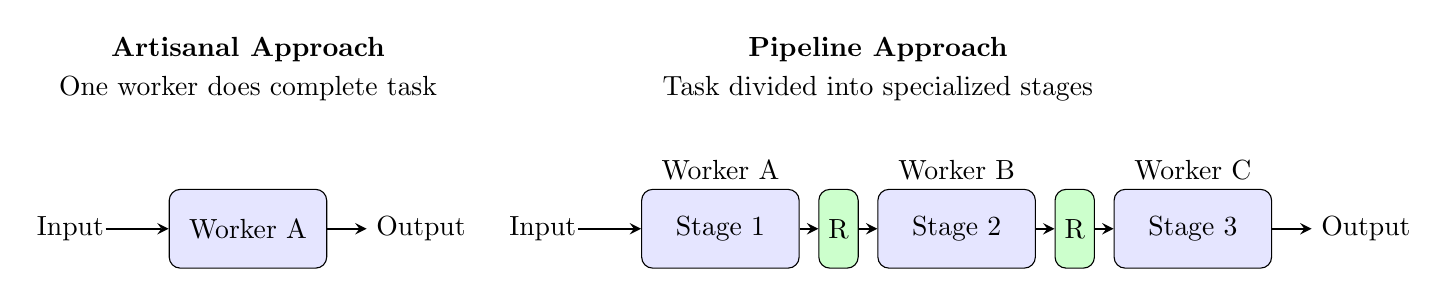
\begin{tikzpicture}[
    stage/.style={rectangle, rounded corners, minimum width=2cm, minimum height=1cm, text centered, draw=black, fill=blue!10},
    reg/.style={rectangle, rounded corners, minimum width=0.5cm, minimum height=1cm, text centered, draw=black, fill=green!20},
    arrow/.style={thick,->,>=stealth}
]


% ARTISANAL APPROACH
\node[above, align=center] at (-4,4.5) {\textbf{Artisanal Approach}};
\node[above, align=center] at (-4,4) {One worker does complete task};

% Single worker doing everything
\node[stage] (workerA) at (-4,2.5) {Worker A};

% Input and output
\node[right] at ($(workerA.east) + (0.5,0)$) {Output};

% Arrows for sequential processing
\draw[arrow] ($(workerA.west) + (-0.8,0)$) -- (workerA.west);
\draw[arrow] (workerA.east) -- ++ (0.5,0);

% PIPELINE APPROACH
\node[above, align=center] at (4,4.5) {\textbf{Pipeline Approach}};
\node[above, align=center] at (4,4) {Task divided into specialized stages};

% Pipeline stages
\node[stage] (stage1) at (2,2.5) {Stage 1};
\node[reg] (reg1) at (3.5,2.5) {R};
\node[stage] (stage2) at (5,2.5) {Stage 2};
\node[reg] (reg2) at (6.5,2.5) {R};
\node[stage] (stage3) at (8,2.5) {Stage 3};

% Input and output
\node[right] at ($(stage3.east) + (0.5,0)$) {Output};

% Horizontal arrows for pipeline flow
\draw[arrow] ($(stage1.west) + (-0.8,0)$) -- (stage1.west);
\draw[arrow] (stage1.east) -- (reg1.west);
\draw[arrow] (reg1.east) -- (stage2.west);
\draw[arrow] (stage2.east) -- (reg2.west);
\draw[arrow] (reg2.east) -- (stage3.west);
\draw[arrow] (stage3.east) -- ++(0.5,0);

\node[left] at ($(workerA.west) + (-0.7,0)$) {Input};
\node[left] at ($(stage1.west) + (-0.7,0)$) {Input};

% Labels for pipeline stages
\node[above] at (stage1.north) {Worker A};
\node[above] at (stage2.north) {Worker B};
\node[above] at (stage3.north) {Worker C};

\end{tikzpicture}

\end{center}
\vspace{1cm}



% \begin{tikzpicture}[font=\small, node distance=1.8cm]
%
% % Artisanal
% \node[draw, rounded corners, minimum width=3.6cm, minimum height=1cm, fill=gray!10] (a1) {Worker does full task};
% \node[below=0.4cm of a1] (alabel) {\textbf{Artisanal:} one worker does everything};
%
% % Arrow to pipeline
% \draw[thick, ->] (a1.east) -- ++(1.2,0) node[midway, above] {};
%
% % Pipeline stages
% \node[draw, rounded corners, fill=blue!10, minimum width=1.7cm, minimum height=1cm, right=2.8cm of a1] (p1) {Stage 1};
% \node[draw, rounded corners, fill=blue!10, minimum width=1.7cm, minimum height=1cm, right=1.8cm of p1] (p2) {Stage 2};
% \node[draw, rounded corners, fill=blue!10, minimum width=1.7cm, minimum height=1cm, right=1.8cm of p2] (p3) {Stage 3};
%
% % Registers
% \node[right=0cm of p1] (r1) {};
% \draw[thick] (p1.east) -- (p2.west);
%
% \node[right=0cm of p2] (r2) {};
% \draw[thick] (p2.east) -- (p3.west);
%
% \node[below=0.4cm of p2] (plabel) {\textbf{Pipeline:} task is split into smaller stages};
% \end{tikzpicture}
\begin{parag}{$ $}
	This means that now, every worker need a third of the original period. So every third of the previous period we are able to output something \textrightarrow we go three time faster.
\end{parag}



\vspace{1cm}

\begin{parag}{Any Advantage Now?}
    The time to compute a single operation is \important{roughly the same} as in the orignal circuit. But now we have new result that are available:
	\begin{itemize}
		\item In the original circuit, \important{every original period $T$}
		\item In the circuit with the registers used for a signle calculation, \important{every $N$ cycles of period $\frac{T}{N}$} \textrightarrow every $T$
		\item In the circuit with the registers where we inject a new computation every cycle, we get:
			\begin{center}
				\textbf{a new result every T/N!}
			\end{center}
	\end{itemize}
	We can generate arbitrarily more result ($N$ large results)?????
\end{parag}
\begin{parag}{Latency and Throughput}
		\begin{definition}[Latency]
	    Time between a computation begins and result is available
	    \end{definition}
		\begin{itemize}
			\item Original circuit: T
			\item Pipelined circuit: $\frac{T}{N} \cdot N =  T$
		\end{itemize}
		\begin{definition}[Throughput]
		Number of results available in the unit time
		\end{definition}
	    \begin{itemize}
			\item Original circui: $\frac{1}{T} = f$
			\item Pipelined circuit: $\frac{1}{\left(\frac{T}{N}\right)} =  \frac{N}{T} = N \cdot f$
	    \end{itemize}
	\begin{framedremark}
	All of this looks great but they only look this great in theory, maybe there is some practical issues...
	\end{framedremark}
\end{parag}
\begin{parag}{Practical Pipelining}
	When we start cutting our circuit, imagine we cut it perfectly by three, then the critical path of this circuit is the maximum between this sub three paths.\\
	Now if the critical path of each subcircuit is magically three, then yes this would works but what if we cannot?\\
	Imagine if we cannot cut perfectly our circuit in third equally subcircuits (which is usually the case), instead of having the critical path being the sum of the three critical paths, we would need to put the maximum critical path among the three multiplied by three.\\
	Furthemore by adding a register we alse take the delay of this register into our critical path.
\end{parag}
    \begin{center}
    \includegraphics[scale=0.2]{screenshots/2025-11-29_8.png}
    \end{center}


\begin{parag}{Usefule Representaiton of the Pipeline Activity}
	So here what we see is that in one cycle we actually do three sub operations, which means that every clock cycle, we are able to output something that take us normaly three clock cycles. This is \important{parallelism}. Not necessarly in the way of how we see it but it still is!
	    \begin{center}
	    \includegraphics[scale=0.2]{screenshots/2025-11-29_9.png}
	    \end{center}
\end{parag}




\subsubsection{Summary}\label{sec:summary:basicpipeline}
\begin{itemize}
	\item \important{Pipelining} consits in splitting a task in smaller 'subtasks', and in performing in \important{parallel} each 'subtask' on a different piece of data
	\item \important{Pipelining} is an extremly general technique to \important{increase the throughput} of a system (circuit, processor, computer, ..)
	\item \important{Pielining does not improve latency} (actually worsens it!)
	\item Therefore, pipelining is only effective when one has to reapeat a job on many pieces of data (signal processing, communication packets, and \important{processor instructions}!)
\end{itemize}









\section{Pipelining}
As said in the previous section, pipelining comes down to splittting our circuit into subcircuits by adding registers. those registers store the informations of the previous subcircuits which makes it free to compute something else. This is that part of pipelining that makes us win a lot of time, we use the pipeline registers to free the previous part of the circuit. As said before there is a lot of backdown which makes it not perfect (see Summary (\ref{sec:summary:basicpipeline}))

\begin{parag}{Pipeline for processor}
    Pipelining is useful only if the activity in object needs to be repeated many time (as in a production line)
	\begin{itemize}
		\item We have plenty of \important{instructions} to execute
	\end{itemize}
	Pipelining needs to split the single activity in object into many subactivities
	\begin{itemize}
	\item We have a \important{good logical split} into fetch decode, execute, etc.
	\end{itemize}
	So we have already done some pipelining in lab b, all the state that we added (load1, load2, etc.) is in some way pipelining.
	
\end{parag}
\begin{parag}{A Simple multicycle CPU}
    
\end{parag}

\begin{center}
    

\begin{tikzpicture}[
    stage/.style={
        circle, draw, fill=gray!10,
        minimum size=2cm, align=center
    },
    arrow/.style={
        -{Stealth}, thick
    },
    note/.style={
        rectangle, rounded corners,
        draw=red!70!black, fill=yellow!20,
        very thick, inner sep=10pt, align=left
    }
]

% Nodes (pipeline stages)
\node[stage] (fetch) {Fetch};
\node[stage, below right=1.4cm and 1.4cm of fetch2] (decode) {Decode};
\node[stage, below left=2.8cm and 3.3cm of decode] (load) {Load};
\node[stage, left=1.4cm of decode] (alu) {ALU};
\node[stage, below left=0.6cm and 0.0cm of alu] (store) {Store};

% Arrows between stages
\draw[arrow] (fetch) edge[bend left] (decode);
\draw[arrow] (load) edge[bend left] (fetch);
\draw[arrow] (store) edge[bend left] (fetch);
\draw[arrow] (alu) edge[bend left] (fetch);
\draw[arrow] (decode) edge[bend left] node[right]{Memory} (load);
\draw[arrow] (decode)  edge[bend left] (alu);
\draw[arrow] (decode)  edge[bend left] (store);

\end{tikzpicture}
\end{center}
\begin{parag}{A Simple schedule}
	At the current moment we are doing pipelining but wihtout any pipeline registers. We are still in  sequential mode.
    \begin{center}
    \includegraphics[scale=0.2]{screenshots/2025-11-29_10.png}
    \end{center}
\end{parag}

\begin{parag}{Pipelining the processor}
    The question we want to ask now is: how far are we from acutally pipelining?\\
	We have already split our finite state machine, what we want now is to actually use those split to gain time:
	\begin{center}
	\includegraphics[scale=0.2]{screenshots/2025-11-29_11.png}
	\end{center}
	So right now we are on the left side of the images, we have every instruction that is still done sequentially. What we want is to go to the right side.
	\begin{framedremark}
	Be careful: the left one which is a \important{finite state machine}, this is not a circuit, this is an abstract representation of the working of the circuit. We will kind of mix them up (the fsm and the circuit) but they are not the same thing.
	\end{framedremark}
	So here what \texttt{F} is storing is all the information of what the cpu needs to do (reading, branching etc.), after \texttt{F} is done (fetch instruction), whatever is activated after this one is going to be put in the second block \texttt{D}. Which means that after \texttt{D} has received the information, \texttt{F} is free again of working on its own \textrightarrow compute the fetch of the next instruction
\end{parag}
\paragraph{No Hardware}%
\label{par:No Hardware}

   In a multicycle processor, some hardware components may be shared across \important{states}:
   \begin{itemize}
	   \item \important{FETCH} typically requires an \important{adder} to increment the program counter
	   \item \important{EXECUTE} naturally needs an \important{ALU}
	   \item They are \important{never used at the same time}, so the ALU can be used to increment the program counter
   \end{itemize}
   In a pipelined processor there cannot be sharing across \important{stages}, in general:
   \begin{itemize}
	   \item All stages are \important{active all the time}
	   \item Hardware needs to be \important{replicated} where appropriate
   \end{itemize}

\paragraph{Two Main Problems}%
\label{par:Two Main Problems}
\subsection{CISC vs. RISC}
	Can we \important{build equally well pipeline} for a Complex Instruction Set Computer as for a Reduced Instruction Set Computer?\\
	And what does this even means complexe, reduced?

\begin{parag}{FSM vs. Pipeline}
	If we look at any loop, at any cycle, it is an instruction, any of the path \important{represent a different instruction}. 
	\begin{itemize}
		\item \textbf{FSM}: The number of state I go from is the number of cycle I will use for each instructions.
		\item \textbf{Pipeline}: Whatever of the instruction, the instruction will have to go through all the pipeline, go through all the state.
	\end{itemize}
	
	\begin{itemize}
		\item \textbf{FSM}: \important{Any path} through the FSM represents the \important{sequence of necessary steps} for the execution of \important{an} instruction
		\item \textbf{Pipeline}: \important{The ordered path} through the pipeline is the \important{sequence of all possible steps} for the execution of \important{any} instruction
	\end{itemize}
	
	\begin{center}
	\includegraphics[scale=0.2]{screenshots/2025-11-29_12.png}
	\end{center}
    
\end{parag}
\begin{parag}{Adding an instruction to a Multi-cycle processor}
    Imagine that we only have one instruction in our multi-cycle cpu \texttt{xor} which result on the red arrow on the above image. What if we need to support the \texttt{add} instruction? To do so we wouldn't need to add any more state, the sequence of steps to execute is the same (fetch instruction, read registers, use the ALU, save result in the register), we just need to an \important{ALU that can perform additions}.
\end{parag}
\begin{parag}{Adding an instruction: not so great instruction to a Multi-cycle processor}
	Imagine now that we want to add the \texttt{lw} instruction, this time we will need a diferent path for this:
	\begin{center}
	\includegraphics[scale=0.2]{screenshots/2025-11-29_13.png}
	\end{center}
\end{parag}
\begin{parag}{Adding Instructions to a Pipeline Processor}
    So for the \texttt{xor} and \texttt{add}, the pipeline doesn't need to be changed.
\begin{center}
    

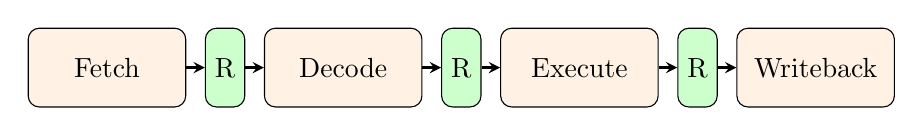
\begin{tikzpicture}[
    stage/.style={rectangle, rounded corners, minimum width=2cm, minimum height=1cm, text centered, draw=black, fill=orange!10},
    reg/.style={rectangle, rounded corners, minimum width=0.5cm, minimum height=1cm, text centered, draw=black, fill=green!20},
    arrow/.style={thick,->,>=stealth}
]


% Pipeline stages
\node[stage] (stage1) at (2,2.5) {Fetch };
\node[reg] (reg1) at (3.5,2.5) {R};
\node[stage] (stage2) at (5,2.5) {Decode};
\node[reg] (reg2) at (6.5,2.5) {R};
\node[stage] (stage3) at (8,2.5) {Execute};
\node[reg] (reg3) at (9.5,2.5) {R};
\node[stage] (stage4) at (11,2.5) {Writeback};

% Horizontal arrows for pipeline flow
\draw[arrow] (stage1.east) -- (reg1.west);
\draw[arrow] (reg1.east) -- (stage2.west);
\draw[arrow] (stage2.east) -- (reg2.west);
\draw[arrow] (reg2.east) -- (stage3.west);
\draw[arrow] (stage3.east) -- (reg3.west);
\draw[arrow] (reg3.east) -- (stage4.west);

\end{tikzpicture}

\end{center}
	But what if we wanted to add the \texttt{lw} instruction again? Then we need to add a new tube into our pipeline:
\end{parag}
\begin{center}
    
    % your TikZ code
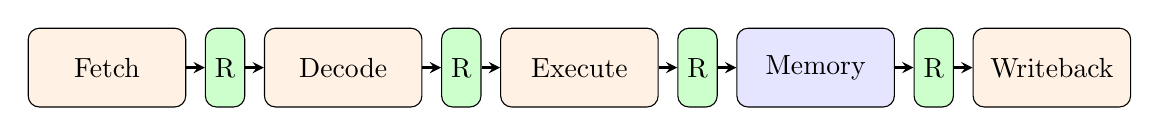
\begin{tikzpicture}[
    stage/.style={rectangle, rounded corners, minimum width=2cm, minimum height=1cm, text centered, draw=black, fill=orange!10},
    newStage/.style={rectangle, rounded corners, minimum width=2cm, minimum height=1cm, text centered, draw=black, fill=blue!10},
    reg/.style={rectangle, rounded corners, minimum width=0.5cm, minimum height=1cm, text centered, draw=black, fill=green!20},
    arrow/.style={thick,->,>=stealth}
]


% Pipeline stages
\node[stage] (stage1) at (2,2.5) {Fetch };
\node[reg] (reg1) at (3.5,2.5) {R};
\node[stage] (stage2) at (5,2.5) {Decode};
\node[reg] (reg2) at (6.5,2.5) {R};
\node[stage] (stage3) at (8,2.5) {Execute};
\node[reg] (reg3) at (9.5,2.5) {R};
\node[newStage] (stage4) at (11,2.5) {Memory};
\node[reg] (reg4) at (12.5,2.5) {R};
\node[stage] (stage5) at (14,2.5) {Writeback};

% Horizontal arrows for pipeline flow
\draw[arrow] (stage1.east) -- (reg1.west);
\draw[arrow] (reg1.east) -- (stage2.west);
\draw[arrow] (stage2.east) -- (reg2.west);
\draw[arrow] (reg2.east) -- (stage3.west);
\draw[arrow] (stage3.east) -- (reg3.west);
\draw[arrow] (reg3.east) -- (stage4.west);
\draw[arrow] (stage4.east) -- (reg4.west);
\draw[arrow] (reg4.east) -- (stage5.west);

\end{tikzpicture}

\end{center}
\begin{parag}{$ $}

	But here this is not really good, imagine that the \texttt{lw} instruction was very rarely used, we would have changed our pipeline, just to add an instruction that is used maybe 0.1\% of the time. We would have slowed our latency by one cycle for an instruction that is barely used, that doesn't seem very efficient...
	\begin{subparag}{The importance if the ISA}
	    Imagine that we want an to have an instruction (we are abusing the RISC-V syntax)
		\begin{lstlisting}[language={[RISC-V]Assembler}]
sub 8(t4), 0(t1), 0(t2)
		\end{lstlisting}
		This is a very bad instruction for us (as RISC-V programmer) but equivalent instruction exists in x86. This is a cisc instruction.\\
		But now if we go back to see how the pipeline for this instruction would look like we can see that this is horrible:\\
		\begin{center}
		\includegraphics[scale=0.2]{screenshots/2025-11-29_16.png}
		\end{center}
		This is very sad, imagine now that we try to execute the instruction \texttt{sub t4, t1, t2}
		There 6 stages that are just \important{useless}
		\begin{center}
		\includegraphics[scale=0.2]{screenshots/2025-11-29_17.png}
		\end{center}
		This is the reason for us to use \important{Reduced Instruction-Set Computer} instead of complex one.
	\end{subparag}
\end{parag}
\begin{parag}{Reduced Instruction-Set Computer}
    Instead of imposing a \important{huge penalty to every simple instruction} by making complex instruction possible, let's \important{have only similarly simple instructions} and build our programs with those.\\
	Instead of writing \texttt{sub 8(t4), 0(t1), 0(t2)} we would divide this instruction into 4 sub instruction:
	\begin{lstlisting}[language={[RISC-V]Assembler}]
lw t3, 0(t1)
lw t5, 0(t2)
sub t3, t3, t5
sw t3, 8(t4)
	\end{lstlisting}
	It turns out that is is not the only way to go, but it is a \important{good one} and we will follow it...
\end{parag}
	\begin{framedremark}
		So the only way to do pipelining efficiently is to have simple, \important{uniform instructions with similar execution paths}.
If instructions differ too much in structure or in the number of steps they require (as in CISC designs), the pipeline must include additional stages to support them, and \important{every instruction—common or rare—pays the cost} of those extra stages. This increases latency, complicates hardware, and wastes cycles.

By contrast, a Reduced Instruction-Set Computer keeps all instructions short, regular, and easy to decompose. This makes it possible to design a pipeline where \important{each stage does a small}, predictable piece of work, and all instructions flow through it smoothly. Complex operations can still be performed, but they are built from multiple simple instructions that the pipeline already supports efficiently.

In short: RISC enables clean pipelining; \important{CISC fights against it}.
That is why modern pipelined processors—and the teaching architecture we study—choose RISC-style instruction sets
	\end{framedremark}




	The question we have and that we have already seen before (see \ref{par:No Hardware}), is: What if instructions are not independent, are we able to execute code \important{correctly}?
\begin{parag}{Simple 5-Stage MIPS Pipeline}
	As an example, we wil take the first pipelined processor to be commercialized: MIP's
	\begin{center}
	\includegraphics[scale=0.2]{screenshots/2025-11-29_18.png}
	\end{center}
	\begin{framedremark}
	The reason of the \texttt{0(t2)} syntax in RISC-V. Whenever accessing or writing to memory, we always go first into \texttt{E} which is execute, which means that we actually get the addition for free here. Even if we didn't want to have that addition we would still need to go through the EXECUTE so might as well always add and add 0 when it is not needed.
	\end{framedremark}
\end{parag}
\begin{parag}{The Laundry Metaphor}
	The point here is when we have a job a sequence of things to do that you want to parallelize, some of those things are just impossible to parallelize. However in the case where parallelizing is hard to do, pipelining is very often the solution.\\
	For example, imagine we haven’t done laundry for a whole month. We would have to run about four loads. We would love to do four of them in parallel but we only have one drier, one washing machine, etc.\\
	The normal way of doing it is to launch one machine wait for it to finish. When it is done we relaunch a new load and dry the one that is clean, etc. 
	We are pipelining our clothes!
	\begin{center}
	\includegraphics[scale=0.2]{screenshots/2025-11-29_19.png}
	\end{center}
\end{parag}
\begin{parag}{Two distinct memory interfaces}
	MIPS (and most modern CPUs) usually separate \important{instruction memory} and \important{data memory}, at least logically in a pipeline. This is called the \important{Harvard architecture}. The reason for this is the following:\\
	At the FETCH stage, we read instruction from memory. In MEMORY stage we also read/write in memory. But remember what we said before (see \ref{par:No Hardware}) we cannot have two stages sharing the same circuit. This means that we need to separate them \textrightarrow instruction memory and data memory. But we cannot split our memory in two. Instead of doing two \important{distinct memories} we actually use \important{two separate caches}.
    \begin{center}
    \includegraphics[scale=0.2]{screenshots/2025-11-29_20.png}
    \end{center}
\end{parag}
\begin{parag}{What is in the Pipeline Registers}
	By definition the pipeline registers stores \important{all data that is needed later}. Every bits, ALU, wire, .. That will be used/needed later in the circuit \textbf{has to be stored} in the registers.\\
	This means that usually those are the things stored in the registers:
    \begin{center}
    \includegraphics[scale=0.2]{screenshots/2025-11-29_21.png}
    \end{center}
\end{parag}
\begin{parag}{Example of Pipelined Execution}
	For this part I won't be screenshooting 10 slides to explain the animations but you can find the explanation in the video \textit{cs-200 --4x. Instruction Level Parallelism Paolo Ienne} at 52:30.
\end{parag}
\subsection{Instruction are not independent}
All of this is nice I agree but imagine the following code:
\begin{lstlisting}[language={[RISC-V]Assembler}]
addi $r0, $r0, 1 
sub $r2, $r0, $r1
\end{lstlisting}
Now try to run this with a pipelined processor... OUCH! In the decode we need a value that is being computed in the EXECUTE, which is far away of being put in the register file.

\begin{parag}{RAW, WAR and WAW Dependences}
	\begin{subparag}{Remark}
	W is for 'write', A is for 'after' and R is for 'read'.
	\end{subparag}
	Dependency are an important thing that we will cover. Let's look at the code:
\begin{lstlisting}[language={[RISC-V]Assembler}]
divd $f0, $f1, $f2 
addd $f3, $f0, $f4
subd $f4, $f5, $f6
addi $f0, $f5, 10
\end{lstlisting}
In our code we have that:
\begin{itemize}
	\item \texttt{add} has a \important{RAW} dependence on \texttt{divd}
	\item \texttt{subd} has a \important{WAR} dependence on \texttt{addd}
	\item \texttt{adddi} has a \important{WAW} dependence on \important{divd}
\end{itemize}
The first dependence is a \important{data} dependency whereas the two other are \important{name} dependencies.\\
All of those dependencies gives us the information that those instructions has to be done sequentially, we have to wait for the other instructions to be done before starting a new one. But wait, is there really an issue with the name dependencies here? Not really, there are \textit{kind of fake}. All we have to do to make them disappear is to change the name of the registers.

As we can see the first one is way more severe that the others.
\end{parag}
\begin{parag}{Data Hazard}
	\begin{center}
	\includegraphics[scale=0.2]{screenshots/2025-11-29_22.png}
	\end{center}
	This is a \important{causality violation}. We try to use a result before it is produced.
    
\end{parag}
\begin{parag}{Data Hazards Solved by Stallig the Pipeline}
	\begin{center}
	\includegraphics[scale=0.2]{screenshots/2025-11-29_23.png}
	\end{center}
	The natural solution to \important{Data Hazards} cause by \important{RAW} dependences is to implement some logic in the processor to stop/repeat the decoding until the required value is available.

	'\important{Stalling}' roughly means introducing \texttt{nop}'s in the pipeline (we are making the code sequential again)

	Due to the rigidity of the pipeline, if one stage is stalled (\texttt{D} in the example), all the preceding ones must be stalled too (e.g., \texttt{F}).
\end{parag}
	So for us what we need to do is those two things:
	\begin{itemize}
		\item We need to understand that we have a poblem (Detecting)
		\item We have to resolve the problem  by running what is missing (Stalling)
	\end{itemize}
\begin{parag}{Detecting}
	The question we will try to answer is how do we see that we have a problem here?

	What we need to check is if the output of the EXECUTE is the same as the input at the DECODE. If they are equal then we have a problem. But this is not all, we also have to check for the other pipeline register, if any \important{pair} is detected then we have a problem.
	\begin{center}
	\includegraphics[scale=0.2]{screenshots/2025-11-29_24.png}
	\end{center}
\end{parag}
\begin{parag}{Stalling}
     We assume that we  know that there is a problem. What we need to do is to let the pipeline compute the current instruction (wihtout fetching a new one) (finish the execute). We would need a multiplexer to before the EXECUTE which would input a nop instruction instead of a rubbish instructions. After that we also need to not enable the pc and to redo the decoding of the instruction with maybe the new value.

	So here we block everything before the DECODE stage. We will block it until nobody tells me that there is an issue.
	\begin{center}
		\begin{center}
		\includegraphics[scale=0.2]{screenshots/2025-11-30.png}
		\end{center}
	\end{center}
	Now we have an example in the course which is on the course \textit{cs-200 -- 4c. Instruction Level Parallelism (cont'd)} on November 2024 at 17:00.
\end{parag}

\begin{parag}{Another Solution}
    What we were doing is adding \texttt{nop} everytime our CPU need to stall from the hardware. But adding those nop is pretty easy to detect before running the program right? so why can't you do it \important{form the software}?
	\begin{center}
	\includegraphics[scale=0.2]{screenshots/2025-11-30_1.png}
	\end{center}
	I means this doesn't look very hard to do in the software right?\\

	But is it better?\\

	Let us take here the line 3 of the left code, the \texttt{xor}. It is independent, which means that in the perspective of the stalling, it comes down to the same thing as a \texttt{nop} instruction right? So we can replace a \texttt{nop} by an independent instructions \textrightarrow we gained one instruction for \important{free}. This is a very nice compiler's problem! If we are able to build a very good compiler that is able to detect those kind of case, this means that we are able to save a pretty good amount of instructions!
\end{parag}
\begin{parag}{Architecture and Microarchitecture}
    What we are doing is \important{microarchitecure}, we are trying to opimize our CPU to do less stalls as possible.
	\begin{itemize}
		\item \textbf{Architecture}: what is in the ISA contract
			\begin{itemize}
				\item Instructions, registers, etc.
			\end{itemize}
		\item \textbf{Microarchitecture}: what is specific of an implementation
			\begin{itemize}
				\item Multi-cycle vs. pipelined, FSM or pipeline structre, etc.
			\end{itemize}
	\end{itemize}
	
	However those solutions we evoked before (reshedule instructions, add \texttt{nop}'s, delay slots) \important{expose typically microarchitectural aspects} (pipeline structure) \important{in the architecture} \textrightarrow the same binary \important{does not run} on different processor
\end{parag}
\begin{parag}{Data Hazard Solved by Forwarding Values}
    So now our pipeline works but can we make it better? For now at every stalling we loose all our progress. \\
	Let us go from the example
	\begin{center}
	\includegraphics[scale=0.2]{screenshots/2025-11-30_2.png}
	\end{center}
	So here we have a \texttt{sub} right after an \texttt{addi}. If we take our pipeline the result of our add is actually computed right after the EXECUTE stage:


\end{parag}
    

\begin{center}
    
    % your TikZ code
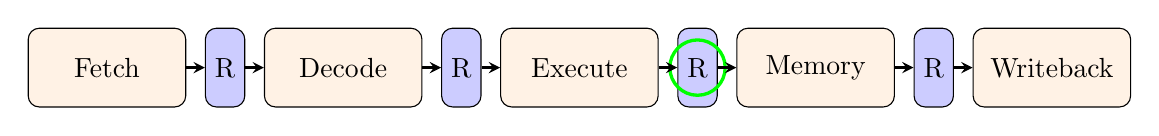
\begin{tikzpicture}[
    stage/.style={rectangle, rounded corners, minimum width=2cm, minimum height=1cm, text centered, draw=black, fill=orange!10},
    newStage/.style={rectangle, rounded corners, minimum width=2cm, minimum height=1cm, text centered, draw=black, fill=blue!10},
    reg/.style={rectangle, rounded corners, minimum width=0.5cm, minimum height=1cm, text centered, draw=black, fill=blue!20},
    arrow/.style={thick,->,>=stealth}
]


% Pipeline stages
\node[stage] (stage1) at (2,2.5) {Fetch };
\node[reg] (reg1) at (3.5,2.5) {R};
\node[stage] (stage2) at (5,2.5) {Decode};
\node[reg] (reg2) at (6.5,2.5) {R};
\node[stage] (stage3) at (8,2.5) {Execute};
\node[reg] (reg3) at (9.5,2.5) {R};
\draw[green, very thick] (9.5, 2.5) circle (10pt);
\node[stage] (stage4) at (11,2.5) {Memory};
\node[reg] (reg4) at (12.5,2.5) {R};
\node[stage] (stage5) at (14,2.5) {Writeback};

% Horizontal arrows for pipeline flow
\draw[arrow] (stage1.east) -- (reg1.west);
\draw[arrow] (reg1.east) -- (stage2.west);
\draw[arrow] (stage2.east) -- (reg2.west);
\draw[arrow] (reg2.east) -- (stage3.west);
\draw[arrow] (stage3.east) -- (reg3.west);
\draw[arrow] (reg3.east) -- (stage4.west);
\draw[arrow] (stage4.east) -- (reg4.west);
\draw[arrow] (reg4.east) -- (stage5.west);

\end{tikzpicture}

\end{center}
\begin{parag}{$ $}
    So our issue here is that we need the output of the EXECUTE at the input of the EXECUTE. Might as well create a bypasse path for this right? 
\end{parag}
\begin{center}
    
    % your TikZ code
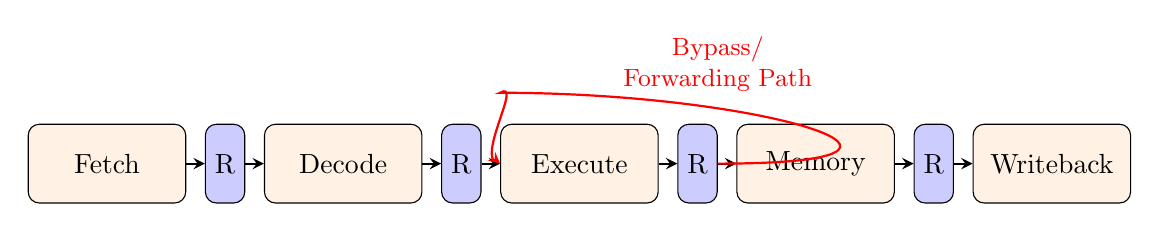
\begin{tikzpicture}[
    stage/.style={rectangle, rounded corners, minimum width=2cm, minimum height=1cm, text centered, draw=black, fill=orange!10},
    newStage/.style={rectangle, rounded corners, minimum width=2cm, minimum height=1cm, text centered, draw=black, fill=blue!10},
    reg/.style={rectangle, rounded corners, minimum width=0.5cm, minimum height=1cm, text centered, draw=black, fill=blue!20},
    arrow/.style={thick,->,>=stealth}
]


% Pipeline stages
\node[stage] (stage1) at (2,2.5) {Fetch };
\node[reg] (reg1) at (3.5,2.5) {R};
\node[stage] (stage2) at (5,2.5) {Decode};
\node[reg] (reg2) at (6.5,2.5) {R};
\node[stage] (stage3) at (8,2.5) {Execute};
\node[reg] (reg3) at (9.5,2.5) {R};
\node[stage] (stage4) at (11,2.5) {Memory};
\node[reg] (reg4) at (12.5,2.5) {R};
\node[stage] (stage5) at (14,2.5) {Writeback};

% Horizontal arrows for pipeline flow
\draw[arrow] (stage1.east) -- (reg1.west);
\draw[arrow] (reg1.east) -- (stage2.west);
\draw[arrow] (stage2.east) -- (reg2.west);
\draw[arrow] (reg2.east) -- (stage3.west);
\draw[arrow] (stage3.east) -- (reg3.west);
\draw[arrow] (reg3.east) -- (stage4.west);
\draw[arrow] (stage4.east) -- (reg4.west);
\draw[arrow] (reg4.east) -- (stage5.west);


% Additional arrow from reg3 east to Execute west (bypass/forwarding path)
\draw[arrow, red, thick] (reg3.east) 
    to[out=0, in=0, looseness=3] 
    ($(stage3.west) + (0,0.9)$) 
    to[out=30, in=180] 
    (stage3.west);
% Label for the bypass path
\node[above, red, align=center, font=\small] at ($(reg3.east) + (0, 0.8)$) {Bypass/\\Forwarding Path};


\end{tikzpicture}

\end{center}
\begin{parag}{ $ $}
    So now we need to add a multiplexer for us two know if we need to take the forwarding path or not.

	However this is a little glitch here:
	What does those register contains? Imagine that:
	\begin{itemize}
		\item We are forwarding E \textrightarrow E (ALU result to the next ALU input)
		\item M \textrightarrow E forwarding (Data memory output or ALU result from M stage)
		\item W \textrightarrow D forwarding (register file writeback in same cycle as read)
	\end{itemize}
	Now the 'glitch' happens in the W \textrightarrow D register file forwarding. The register file must:
	\begin{itemize}
		\item \important{write} a value in W stage
		\item \important{read} it in the D stage of the next instruction
	\end{itemize}
	\begin{center}
	    \textbf{in the same clock cycle}
	\end{center}
	This is just \important{impossible}.\\
	In order to resolve this issue we have to check in the DECODE if the register that we took from is valid or not \textrightarrow we need some bits of information that tell us wether the register we are using is valid or not.\\
	Us from two pages ago would take those valid bits as redundancy, we need the \important{value} and \important{register}.\\
	We then check with a multiplexer if the register value is rubbish or is it valid. If it is rubbish we then use one of the red arrow, else the value.
\end{parag}


\begin{parag}{Classic MIPS pipeline}
    For a classic 5-stage pipeline with \important{all forwarding paths}:
	\begin{itemize}
		\item E \textrightarrow E, M \textrightarrow E
		\item W \textrightarrow D
	\end{itemize}
	The \important{register-file forwarding} (W \textrightarrow D) is a special case:
	\begin{itemize}
		\item During \textbf{W}, registers are written in the \important{first half} of the cycle
		\item During, \textbf{D}, registers are read in the \important{second half} of the cycle.
	\end{itemize}
	\begin{subparag}{How can we divide our clock cycle}
	    The way of doing it is use level sensitives, we write in our register-file when there is a rising edge of the clock, we read our register-file when there is a lower edge of the clock. The write occurs when \texttt{clk} is high, the read occurs when the \texttt{clk} is low.
	\end{subparag}
	This means that a register can be correctly written and read in the same cycle
	\begin{center}
	\includegraphics[scale=0.2]{screenshots/2025-11-30_3.png}
	\end{center}
	Example again on \textit{cs-200 4c. Instruction Level Parallelism November 20, 2024 at 1:05}
	But here we have saved a lot of stalling, our pipeline is almot perfect. The only stalling we still get is when we are decoding a register that is in E but need to be loaded for instance:
	\begin{lstlisting}[language={[RISC-V]Assembler}]
lw r9, 0(r7)
sub r3, r9, r1
	\end{lstlisting}
	So here \important{most of the stalls} are removed.
	\begin{subparag}{Remark}
	    This is only something that can be done in hardware, this is not possible to do from a software perspective.
	\end{subparag}
\end{parag}


\subsubsection{Structural Hazards}
\begin{definition}[structural hazard]
A \important{structural hazard} happens when different instructions compete for the same ressource (e.g., pipeline stage)

It is a \important{ressource conflict}.
\end{definition}
Our structural hazards \important{canot happen} in our pipeline. If we did not stall also instructions following one missing an operand, we could have structural hazards.
	\begin{center}
	\includegraphics[scale=0.25]{screenshots/2025-11-30_4.png}
	\end{center}

	But what happen if we have a \important{cache miss}? If we have a data cache miss, then we have to wait for the cache to responds, all the previous stage are stalling, the W stage on the other hand can advance (the same principle goes for the F stage).

	\begin{parag}{What about miss on both side?}
		So here if we have two miss then we have a \important{structural hazard} on main memory. The way of solving them is to let the most right miss have the priority.
	\end{parag}


\begin{parag}{Control Hazard}
	Let us take for instance this code:
    \begin{center}
    \includegraphics[scale=0.2]{screenshots/2025-11-30_5.png}
    \end{center}
	Here we have a big issue, after the branch instruction, what should we fetch? We don't know which instruction we should have fetched. This is a \important{causality violation}
\end{parag}
\begin{parag}{Control hazard solved by stalling}
    So here the easy way of solving it is to stall the pipeline when we have a branch. 
	\begin{center}
	\includegraphics[scale=0.2]{screenshots/2025-11-30_6.png}
	\end{center}
	Similarly to the way we solve data hazards, we can \important{stall the pipeline} (F), one it is discovered, after \textbf{D}, that an instruction was a branch, and this \important{until the branch is resolved}.\\

	If, for instance the correct address of the next instruction is know at the end of the E stage, \important{2 cycles are lost every branch}
\end{parag}
\begin{parag}{Fetching and decoding do not do any damage}
	Maybe we can have a slightly better view of that. After all we are not fetching rubbish in the first case. There is a possibility that the instruction that we have fetched is actually correct.
    \begin{center}
    \includegraphics[scale=0.2]{screenshots/2025-11-30_7.png}
    \end{center}
	\begin{itemize}
		\item Fetching or decoding a wrong instruction does not create any problem, provided that the instruction is not also \important{executed}
		\item If the outcome of the branch is known at the end of the E stage, we can \important{wait} until then to \important{conditionally kill} the following two instructions in the pipeline \important{if the branch happens to be taken}
		\item Now \important{2 cycles are lost only for taken branches} and \important{none is lost for nontaken ones}
	\end{itemize}
\end{parag}
\begin{parag}{Another solution}
    As we have seen for data hazard, we  can also use the software in order to resolve those hazards. We could just add \texttt{nop} at this good place which would resolve our hazard.
\end{parag}
\begin{parag}{Control Hazard Solved by Delay Slot}
	\begin{center}
	\includegraphics[scale=0.2]{screenshots/2025-11-30_8.png}
	\end{center}
	Alternatively, we can \important{modify the definition of the architecture} and decide that \important{the two instructions following a branch are executed in any case} (branch taken or not) as if they were before (same thing as in cs-328). Thse instructions after the branches are called \important{delay slots}, before when a branch happened we added \texttt{nop}, so might as well try to compute someting instead right? 
	But now our code becomes \important{counterintuitive}, we execute code maybe for nothing.
	\begin{subparag}{Remark}
	    MIPS did it as some others, but quite rare in current architectures
	\end{subparag}
\end{parag}
\begin{parag}{Use of Delay Slots}
	A simple way of using delay slots is to use them for \texttt{nop}'s-- but then it is not better than stalling the pipeline. A better idea is to put there instructions which precede the branch and on which the branch has \important{no dependence}.
	Suppose an architecture with two delay slots:
	\begin{lstlisting}[language={[RISC-V]Assembler}]
sub r2, r0, r7
mul r1, r6, r7
add r5, r3, r4 
beq r0, r1, loop 
nop
nop
lw r8, 12(r9)
	\end{lstlisting}
	Then this can be turned into:
\begin{lstlisting}[language={[RISC-V]Assembler}]
mul r1, r6, r7
beq r0, r1, loop 
sub r2, r0, r7 
add r5, r3, r4 
lw r8, 12(r9)
\end{lstlisting}
We use some instructions that is independent to fill the nop instructions
\end{parag}



\begin{parag}{Branch Prediction}
	\begin{itemize}
		\item A better strategy is to \important{guess the branch outcome} and fetch the corresponding instruction (either the next instruction or the branch destination, but not nessarily the former)
			\begin{itemize}
				\item If the guess is correct, \important{no cycle is lost}
				\item If the guess is wrong, what has been fetched and decoded is thrown away (\important{squashed})
			\end{itemize}
		\item Branch predictors of modern processors are extremly sophisticated:\\
			dynamic predictors \important{learn from previous executions} of branch...
			\item Complex predicots can be \important{correct up to 95-99\%} of the time
			\item The quality of branch predictors has made architectures with delay slots extremly rare
	\end{itemize}
\end{parag}




\subsubsection{Three Types of Hazards Hinder Pipelining}
\begin{parag}{Solutions}
    \begin{subparag}{Data Hazards}
        \begin{itemize}
			\item Forwarding paths, wherever possible
			\item Stalls in all other cases
        \end{itemize}
    \end{subparag}
	\begin{subparag}{Control Hazards}
	    \begin{itemize}
			\item Delay slots, if the architecture allows it
			\item Branch prediction, to try to do the right thing
			\item Stalls, if not
	    \end{itemize}
	\end{subparag}
	\begin{subparag}{Structural Hazards}
	    \begin{itemize}
			\item Rigid pipelines which cannot have structural hazards by construction
			\item Stalls, otherwise
	    \end{itemize}
	    
	\end{subparag}
\end{parag}



\section{Dynamic Scheduling}

\begin{parag}{Starting point}
    As we have seen before, processor has first been \important{sequential multicycle processor}. Now we wanted to replace it with something else: \important{pipelined processor}.
	\begin{center}
	\includegraphics[scale=0.2]{screenshots/2025-12-03.png}
	\end{center}
	For instance, 5-stage pipeline with all forwarding paths. Typical of \important{MIPS} and \important{RISC-V}.
	The issue with this is that \important{all instructions} has to go through \important{all the stages} $\implies$ we need a very small ISA (MIPS, RISC-V).
	The other issue is that pipelined need \important{independence}. Every circuits in each stage has to be used \important{only in that stage}.
	This is the simplest form of \important{Instruction Level Parallelism} (ILP): several instructions are now executed at once.
\end{parag}
\begin{parag}{Simple Pipelining}
    The scope if \important{parallelism is limited}:
	\begin{itemize}
		\item \important{Data hazards} limit the usability of the pipeline:
			\begin{itemize}
				\item Whenever the next instruction cannot be executed, the pipeline is stalled and no new useful work is done until the 'problem' is solved (e.g., cache miss)
			\end{itemit
		\item \important{Control hazards} limit the usability of the pipeline
			\begin{itemize}
				\item Must squash fetched and decoded instruction followig a branch
			\end{itemize}
		\end{itemize}
	\end{itemize}
\end{parag}
\begin{parag}{Rigid Sequencing}
    \begin{itemize}
		\item Special 'slots' for everything even if sometimes useless (e.g. M)
		\item Every instruction must be \important{coerced to the same framework} (floating point vs. integer)
		\item Structural hazards avoided 'by construction'
    \end{itemize}
	This means that if we need some floating point arithmetic then we are a bit lost on our RISC processor. We would need to implement the floating point in software (which is slower).
\end{parag}

\end{parag}
\paragraph{Dynamic Scheduling: The Idea}%
\label{par:Dynamic Scheduling: The Idea}
Let us for instance take a look at the code:
\begin{lstlisting}[language={{RISC-V}Assembler}]
divd $f0, $f2, $f4
addd $f10, $f0, $f8
subd $f12, $f8, $f14
\end{lstlisting}
Here the instruction \texttt{divd} is a long-running instruction which hurt our feeling...it makes our program \important{stalls} for the next instruction \texttt{add f10, f0, f8} which need the value \texttt{f0}. However as we can see the instruction \texttt{subd} is completely independent of the two above. As we have seen before, maybe a way of resolving the stalling is by using a 'smart' compiler which would put the \texttt{subd} instruction between those two. However here our \texttt{divd} takes a long time but how much? how many cycles? We cannot know right? Imagine having a \texttt{load} instruction we wouldn't even know!
\begin{theoreme}
Relax a fundamental rule: instructions can be executed \important{out of program order} (but the result must still be \important{correct}).
\end{theoreme}

\begin{parag}{Break the Rigidity of the Basic Pipelining}
    For us we need:
	\begin{itemize}
		\item \important{Continue fetching and decoding} even and especially if one cannot exevcute previous instructions
		\item \important{Keep writeback waiting} if there is a structural hazard, without slowing down execution.
	\end{itemize}
\end{parag}
\begin{parag}{Solution}
    The solution here is the \important{splits the tasks} in independent units/pipelines
	\begin{itemize}
		\item \important{Fetch and Decode}
		\item \important{Execute}
		\item \important{Writeback}
	\end{itemize}
\end{parag}
\begin{parag}{Dynamically Scheduled Processor}
	So now the we don't have to go through one big pipeline. Now we break our previous big pipeline into smaller pipeline. We may have a big pipeline for floating point double and a smaller one for 32 bits floating point. 
    \begin{center}
    \includegraphics[scale=0.2]{screenshots/2025-12-03_1.png}
    \end{center}
	So what is going here is we create a big Execution unit with all the possible instruction (memory, alu, etc.). We then wire them back into our decode just as we did before. Now everything that produce a result we bring it back \important{where} there is a possible use of it.
	
\end{parag}
\begin{framedremark}
Here what we have is still a finite state machine. The reason why we don't present it as one is that the number of state that is can have is enormous. It the a combinatorial calculation between all the state F, D, E/M1, .., W.
\end{framedremark}

\subsubsection{Problems to solve}
Now we have a kind of big work to do, all the previous issues that we had already solved come back again at us here:
\begin{parag}{Structural Hazards}
	\begin{itemize}
		\item Are the required resources available?
		\item New problem: previously handled by rigid pipeline
	\end{itemize}
\end{parag}
\begin{parag}{RAW Data Hazards}
    \begin{itemize}
		\item Are the operands ready to start execution
		\item Old problem
    \end{itemize}
\end{parag}
\begin{parag}{WAR and WAW Data Hazards}
	\begin{itemize}
		\item The new data overwrite something which is still requires?
		\item WAW is a completely new problen -- impossible before, WAR often cannot occur
	\end{itemize}
\end{parag}

\begin{parag}{Raw Data Hazards}
    Let us start with this one. This problem comes fron the \texttt{RS} register from the previous picture. Maybe what we read the register and the value from it is false. We want  to erase it. The solution here is to use a \important{Reservation Station}
\end{parag}
\begin{parag}{Reservation Station}
	\begin{definition}[Reservation station]
	checks that the \important{operands are available} (RAW) and that the \important{Execution Unit is free} (Structural Hazards), then starts execution.
	\end{definition}
    \begin{center}
    \includegraphics[scale=0.2]{screenshots/2025-12-03_2.png}
    \end{center}
	So here for instance the \texttt{ALU3} means that the value we are waiting for will be the result of the \texttt{ALU3} instruction im the reservation stations.
	\begin{subparag}{The parking lot}
	    We can see our Reservation stations as a \important{parking lot} instead of having car we have instructions waiting to be ready. Everytime one is ready then we launch it. This is a completely \important{unordered} 'data structure'.
		On the bottom we have a ALU that is ready to compute something \important{every cycles}.
		On the top then we have all the come back pipe which comes to us and tell for intsnace 'I am the result of the MUL3 computation' we then ask ourself if any of us (instructions) is waiting for the \texttt{MUL3} result.
	\end{subparag}
\end{parag}
\begin{center}
    
\scalebox{0.7}{
\begin{tikzpicture}[
    node distance=2cm,
    box/.style={
        draw,
        minimum width=6cm,
        minimum height=2.5cm,
        align=center,
        fill=red!20
    },
    textnode/.style={
        align=center,
        text width=6cm
    },
    >=Stealth
]

% Reservation Station box
\node[box] (RS) {Reservation Station};

% Top-left text
\node[textnode, above left=1.7cm and -0.3cm of RS] (FD) {
    \textbf{\underline{Fetch\&Decode Unit and Register File}} \\
    (1) Fetched operation descriptions and \\
    (2a) known operands (from RF) \\
    or (2b) source-operation tags
};

% Top-right text
\node[textnode, above right=1.7cm and -0.3cm of RS] (EU) {
    \textbf{\underline{All Execution Units}} \\
    (1) Tags of the executed operations \\
    and (2) corresponding results
};

% Bottom text
\node[textnode, below=2cm of RS] (DEU) {
    \textbf{\underline{Dependent Execution Unit}} \\
    (1) Description of operations ready to execute \\
    with (2) corresponding tags and (3) operands
};

% Arrows
\draw[->, thick] (FD) -- (RS);
\draw[->, thick] (EU) -- (RS);
\draw[->, thick] (RS) -- (DEU);

\end{tikzpicture}
}



\end{center}

\begin{parag}{What is a Reservation Station?}
A \important{reservation station} is a small buffer inside the processor that holds
instructions after they have been decoded but \important{before} they are executed.
Its purpose is to allow the CPU to execute instructions \textbf{out of order}
without violating the correctness of the program.

A reservation station entry contains:
\begin{itemize}
    \item the \textbf{operation} to execute (e.g.\ \texttt{add}, \texttt{mul}), 
    \item the \textbf{operands}, if they are already available,
    \item or \textbf{tags} indicating that the operand is not available yet,
    \item and the \textbf{destination tag} where the result must later be written.
\end{itemize}

The idea is simple: an instruction does \important{not} need to wait for its
operands in the decode stage. Instead, it is placed in a reservation station
entry, even if some operands are missing. The entry then ``listens'' to all
execution units. Whenever a unit finishes and broadcasts a result together with
its tag, each reservation station checks whether it was waiting for that value.

If an entry collects \important{all} its operands, then that instruction is marked
as \textbf{ready}. As soon as the corresponding execution unit becomes free,
the reservation station dispatches the instruction to it.

In short:
\begin{itemize}
    \item It solves \textbf{RAW hazards} by waiting for the true operands.
    \item It helps avoid \textbf{structural hazards} by checking that the execution unit is free.
    \item It enables \textbf{out-of-order execution}: instructions no longer need to
          wait in program order if they already have what they need.
\end{itemize}

A reservation station therefore acts as a \important{smart waiting room} for
instructions: they enter as soon as they are decoded, wait only for the data
they require, and are issued to execution as soon as they are ready.
\end{parag}
So here our read after write issue is gone. But the WAR or WAW are not resolved. The question the Prof. asked was:
\begin{center}
    Why don't we use something simpler for our tag (e.g., the register name)?
\end{center}
Our register are not unique, this would work only if we were in an ordered program where each instruction are followed by the next one. If that was the case then yes this would work because as the register t4 we would have the latest value of t4 which is the one we need.
But what happens if we are in an unordered instruction table (Reservation stations)? Then in that case it could be possible that there is a previous value that is not the correct one in t4, t4 would not be unique.

We need \important{unicity} we have to be sure that when calling a tag then the value of this tag \important{has to be unique}.

So why don't we use the program counter as a tag? By using it then we have a unique identifier for each value right? But what if we have a loop, then for the same pc we would still have two different values.

\begin{parag}{WAW and WAR}
    Those hazard were not really possible in a simple pipeline (by construction). However here this is different, for instance:
	\begin{center}
	\includegraphics[scale=0.2]{screenshots/2025-12-03_4.png}
	\end{center}
	So here we have a new issue. The solution for this would be for instance to rename our register like:
	Given this code
	\begin{lstlisting}[language={{RISC-V}Assembler}]
divd f0, f1, f2 
addd f3, f0, f4 
subd f4, f5, f6  #create issue with the f4 of the previous instruction
adddi f0, f4, 10 #create issue with the f4 of the previous instruction
	\end{lstlisting}
	We can change it to:
\begin{lstlisting}[language={{RISC-V}Assembler}]
divd f0, f1, f2 
add f3, f0, f4 
subd f30, f5, f6 
f29, f30, 10
\end{lstlisting}
	But here our reservation station comes down pretty much as renaming each register as the tag.
	\begin{itemize}
	   \item Unavailable operands are identified by the \important{name of the reservation station} in charge of the originating instruction
	   \item \important{Implicit register renaming}, thus removing WAR and WAW hazards
	   \item New results are seen at their inputs through special result bus(es)
	   \item Writeback into the registers can be in-order or, to some extent, out-of-order
	\end{itemize}
\end{parag}

\subsection{Dynamically Scheduled Processor}
So here what we get at the end is:
\begin{center}
\includegraphics[scale=0.3]{screenshots/2025-12-03_5.png}
\end{center}
What we here as an issue still is how do we know where to write in the register file, we need to be careful about our ordering in our register file. This is the commit unit's job.
\begin{parag}{Our-of-order Commitment and Exceptions}
	\begin{itemize}
		\item Excpetion handlers should know exaclty where a problem has occured, especially for \important{nonterminating exceptions} (e.g., page fault)
		\item Of course, one assumes that everything before the faulty instruction was executed and everything after was not
		\item With dynamic execution it might no longer be true...
	\end{itemize}
\end{parag}
\begin{parag}{Problems with exceptions}
    Now we have an issue again with excpetions:
	\begin{subparag}{Precise exceptions}
	    Reordering at commit; user view is that of a fully in order processor
		\begin{lstlisting}[language={{RISC-V}Assembler}]
andi t4, t2, 0xff # good code
andi t5, t4, 0xff # good code
addi v0m t5, 1  # good code
srl t2, t2, 8 # good code
-> lw t3, 8(t6) # now we have our exception
andi t4, t3, 3  # bad code
addi t0, t0, 4 # bad code
addi t1, t1, 4 # bad code
		\end{lstlisting}
		So now we need to come back from where were at the exception. To do so we need to save the pc of where the exception has happened we already have it and returning to it is already implemented (the \texttt{ret} in RISC-V).
		
	\end{subparag}
	\begin{subparag}{Imprecise exceptions}
		\begin{itemize}
			\item No reordering; out-of-order completion visible to the user
			\item The OS/programmer must be aware of the problem and take appropriate action (e.g., execute again the complete subroutine where the problem occured)
		\end{itemize}
		\begin{lstlisting}[language={{RISC-V}Assembler}]
andi t4, t2, 0xff # good code
andi t5, t4, 0xff # bad code
addi v0m t5, 1  # bad code
srl t2, t2, 8 # good code
-> lw t3, 8(t6) # now we have our exception
andi t4, t3, 3  # bad code
addi t0, t0, 4 # good code
addi t1, t1, 4 # bad code
		\end{lstlisting}
		Now here we are not able to jump again, if we were, yes our program would run again fine but then that addi here has already been computed (\texttt{addi t0, t0, 4}) would be refetched again which would make our \texttt{to} incremented two times!
	\end{subparag}
\end{parag}
\begin{parag}{Solution}
    The way of solved this issue is to add a new buffer between the output and the register file:
	\begin{center}
	\includegraphics[scale=0.3]{screenshots/2025-12-03_6.png}
	\end{center}
	This one is pretty different from the other buffer. This one \important{has to be ordered}. This buffer works kind of like our pipeline registers.
\end{parag}




\section{Scheduling Examples}
The is the program that we will want to run:
\begin{lstlisting}[language={{RISC-V}Assembler}]
lw x1, 0(x5)
addi x5, x1, 1
lw x1, 0(x6)
add x3, x8, x5
subi x2, x6, 1
subi x4, x3, 5
add x3, x2, x4
lw x2, 0(x7)
or x4, x2, x1
subi x7, x3, 9
\end{lstlisting}
\begin{parag}{Goal}
    The goal for us with this section will be:
	\begin{itemize}
		\item Determine the \important{execution schedule} for this code in five different architectures
		\item \important{Compare the number of cycles} required by the five architectures
		\item \important{Compute the CPI} (and IPC) of all architectures on this program
	\end{itemize}
\end{parag}
\subsection{Architecture 1}
For this first architecture, we will use a \important{multicycles} processor without any pipelining. The execution latencies are the following:
\begin{itemize}
	\item ALU operations \textrightarrow 4 cycles
	\item Memory operations \textrightarrow 6 cycles
\end{itemize}
So for us here this is very simple to count the number of instructions so here there are three load and 7 ALU operations:
\begin{align*} 3 \cdot 6 + 7 \cdot 4 = 46 \end{align*}
What we also want to compute here is the average cycles per instructions:
\begin{align*} \frac{46}{10} = 4.6 \end{align*}

\subsection{Architecture 2}
Here we will have a \important{6-stage pipelined} processor without any forwarding paths
\begin{center}
\includegraphics[scale=0.2]{screenshots/2025-12-12.png}
\end{center}
So here we have two cycles more that every \important{non load/store instructions} has to go through. It can be even worse if we have dependency.\\ 
The way of doing it is step be steps: first the first instruction \textrightarrow it doesn't depend on anything so we can just put without any dependency. Then we check the second instruction if it has any dependency \textrightarrow it has one: the \texttt{x1} this means that we will need to wait until the writeback for the next instruction is done. we will need to stall our processor four times. Because this is a rigid pipeline, everything in our processor is stalling so we need to fetch again and again our value (even if it is correct) until our CPU is again free. So for the second instructions, we have fetched 5 times the correct value.\\
At the end here if we continue until the end of the program we get the following:
\begin{center}
\includegraphics[scale=0.2]{screenshots/2025-12-12_1.png}
\end{center}
We needed \important{33} cycles \textrightarrow
\begin{align*} \text{CPI} =  \frac{33}{10} = 3.3 \end{align*}

\subsection{Architecture 3}
Now we still have a \important{6-stage pipelined} with \important{some forwarding paths}
\begin{itemize}
	\item E \textrightarrow E, M2 \textrightarrow E
	\item W \textrightarrow D
\end{itemize}
\begin{center}
\includegraphics[scale=0.2]{screenshots/2025-12-12_2.png}
\end{center}
Let us take the first instruction \texttt{lw x1, 0(x5)}. The result of this instruction will be available after M2 right? which means that as soon as M2 has finished his job \textrightarrow we have that the result is direclty transfered into the Execution stage (M2 \textrightarrow E). In comparaison of what we did before; we gain \important{one whole} cycle.
\begin{center}
\includegraphics[scale=0.2]{screenshots/2025-12-12_3.png}
\end{center}
If we count the number of cycles needed we get $21$:

\begin{align*} \text{CPI} =  \frac{21}{10} = 2.1 \end{align*}

\begin{lstlisting}[language={{RISC-V}Assembler}]
1: lw x1, 0(x5)
2: addi x5, x1, 1
3: lw x1, 0(x6)
4: add x3, x8, x5
5: subi x2, x6, 1
6: subi x4, x3, 5
7: add x3, x2, x4
8: lw x2, 0(x7)
9: or x4, x2, x1
10: subi x7, x3, 9
\end{lstlisting}

\subsection{Architecture 4}
We still have a pipelined processor (the last one), but here we have \important{all the forwarding paths}.
\begin{center}
\includegraphics[scale=0.2]{screenshots/2025-12-12_4.png}
\end{center}
Here the first instruction doesn't change from what we did with the third processor.
The fourth and the second instruction has a dependency, but this times instead of having to stall the processors we can actually retrieves our value from M1 which makes us gain one cycle. If we following the same principle for all the execution we get:
\begin{center}
\includegraphics[scale=0.2]{screenshots/2025-12-12_6.png}
\end{center}
If we count the number of cycle needed we get 19 which is very good:
\begin{align*} \text{CPI} =  1.9 \end{align*}

\subsection{Architecture 5}
Now we have a \important{Dynamically scheduled}, out-of-order (OOO), unlimited RS and ROB size
\begin{itemize}
	\item 1 ALU (latency 1) + 1 Memory Unit (latency 3)
\end{itemize}
\begin{center}
\includegraphics[scale=0.2]{screenshots/2025-12-12_7.png}
\end{center}
So we also need a Reservation Station, one for each execution Unit, in our context, we have two executions unit
\begin{center}
\includegraphics[scale=0.2]{screenshots/2025-12-12_8.png}
\end{center}
We also need a reordering Buffer (ROB)
\begin{center}
\includegraphics[scale=0.2]{screenshots/2025-12-12_9.png}
\end{center}

\paragraph{'to do list' for simulating Dynamically Scheduled Processor}%
\label{par:'to do list' for simulating Dynamically Scheduled Processor}
\begin{itemize}
	\item At the beginning of each cycle
		\begin{itemize}
			\item \textbf{E phase} -- Issue ready instructions:
				\begin{itemize}
					\item From all RSs, issue as many ready instructions as there are FUs available
				\end{itemize}
			\item \textbf{W phase} -- Writeback results in order:
				\begin{itemize}
					\item Remove top entry from ROB if completed (\textbf{ONLY THE TOP})
				\end{itemize}
		\end{itemize}
		\item At the end of each cycle
			\begin{itemize}
			\item \textbf{D phase} -- Load result of decoding state:
				\begin{itemize}
					\item To the relevant RS, including ready register values
					\item To the ROB, to prepare the placeholder for the result 
				\end{itemize}
			\item \textbf{E phase} -- Broadcast results from all FUs:
				\begin{itemize}
					\item To all RSs (incl.deallocation of the entry)
					\item To all the ROB
				\end{itemize}
			\end{itemize}
\end{itemize}
\begin{framedremark}
The explanation on how to run this is 14:00 in \textit{CS-200 -- 4e. Instruction Level Parallelism (cont'd)} from the 4th December
\end{framedremark}
So here we have the first two cycles which are the same as the usual pipelined processor, the. We have decoded the first instruction which is a load words with the arguments 0 and 555. So we then put the instruction into the reservation table for the memory unit at for instance \textbf{MEM2}.
\begin{center}
\begin{tabular}{c|c|c|c|c|c|c|}
	& & Op & Tag1 & Tag2 & Arg1 & Arg2 \\
	\hline 
	\textbf{MEM1} & & & & & &  \\
	\hline
	\textbf{MEM2} &e & lw & -  & - & 0  & 555 \\
	\hline
	\textbf{MEM3} & &  &  & &  & \\
	\hline
\end{tabular}
\end{center}
\begin{framedremark}
The order or where we put it in the reservation table doesn't matter
\end{framedremark}
The decodin also need to keep track of the fact that this instruction exists \textrightarrow is also put the information in the reorder buffer. We put the instruction at the top of the ROB with the following informations:
\begin{itemize}
	\item PC = 1
	\item EX = 0
	\item At the current time, the tag we are using for this instructions \important{must be unique} here MEM2 \important{has to be unique}
	\item so the register is \texttt{x1}
	\item The address is nothing because we don't have to write to the address
	\item We don't know the value at the current value
\end{itemize}
We do now to the next cycle: we check if there is any tag in our MEM2 station, there is none (obviously because this is the first instruction) therefore we can enter into the memory unit. Has we have said before it has a latency of three which means that this instruction is gone for three cycles (there is no going back).

Should we erase this instruction from the reservation table? I mean we don't use it now so why should we keep it?

But if we let someone take our parking spot, then MEM2 becomes the new instruction right? 

But we are not done with the previous MEM2, so we would have a mismatch of MEM2.\\

We need to add a bit of 'state' to know what is up with our tag. the bit would be 1 if we are currenlty executing the instruction else 0.

At the same time the second instruction also is decoded at the second cycle. so this is an immediate instruction \textrightarrow we only need to check one register \texttt{x1}. We check the ROB if we see that there is \texttt{x1} then we know that it is not ready. As we can see there is \texttt{x1} \textrightarrow we check tat tag MEM2 and we store this tag in our reservation station of the ALU unit. we have for instance
\begin{center}
\begin{tabular}{c|c|c|c|c|c|c|}
	& & Op & Tag1 & Tag2 & Arg1 & Arg2 \\
	\hline 
	\textbf{ALU1} & & & & & &  \\
	\hline
	\textbf{ALU2} & & & & & &  \\
	\hline
	\textbf{ALU3} & & add & MEM2 & - &  - & 1 \\
	\hline
\end{tabular}
\end{center}


\begin{center}
\includegraphics[scale=0.3]{screenshots/2025-12-12_10.png}
\end{center}
\begin{parag}{Solution}
    This is the ALU rs
\begin{center}
\begin{tabular}{c|c|c|c|c|c|c|}
	& & Op & Tag1 & Tag2 & Arg1 & Arg2 \\
	\hline 
	\textbf{ALU1} & & & & & &  \\
	\hline
	\textbf{ALU2} &w  &add & -  & -  & 257 & 93 \\
	\hline
	\textbf{ALU3} & & sub & - & - &  456 & 1 \\
	\hline
\end{tabular}
\end{center}
And this is the MEM rs
\begin{center}
\begin{tabular}{c|c|c|c|c|c|c|}
	& & Op & Tag1 & Tag2 & Arg1 & Arg2 \\
	\hline 
	\textbf{MEM1} & & & & & &  \\
	\hline
	\textbf{MEM2} & e & lw & -  & -  & 456 & 0 \\
	\hline
	\textbf{MEM3} & &  &  &  &  &  \\
	\hline
\end{tabular}
\end{center}
This is the ROB

\begin{center}
\begin{tabular}{|c|c|c|c|c|c|}
	 Excpt. & PC & Tag & Register & Address & Value \\
	\hline 
	0 & & & & &  \\
	\hline
	0 & 2 & - & x5  & -  & 93 \\
	\hline
	0 & 3 & MEM2  & x1 &  -  & ??? \\
	\hline
	0 & 4 &ALU2  &  x3  &  - &  ???\\
	\hline
	0 & 5 & ALU3 &  x2  & - & ??? \\
	\hline
\end{tabular}
\end{center}

\end{parag}








\section{Besides and Beyond Superscalars}
So far we used to way two optimize our processor: pipelined and dynamic scheduling, for this lecture we will see if we can go a completely different way of what we have done before. 

\begin{parag}{Content of this lecture}
    \begin{itemize}
		\item Superscalar processors
		\item Speculative execution
		\item Simultaneous multithreading
		\item Nonblocking caches
		\item Very long instruction word (VLIW) processors
    \end{itemize}
\end{parag}
\begin{parag}{To this day}
    So for us our processor look like this:
	\begin{center}
	\includegraphics[scale=0.2]{screenshots/2025-12-13_3.png}
	\end{center}
	We have two big \important{seperate parts} in our  circuit:\\
	\begin{itemize}
		\item The ordered part: between the commit unit and the register file, instruction Fetch and decode unit
		\item The unordered part: the reservation stations and all the unit
	\end{itemize}
	The limits we have is for instance imagine we have 3 alu instructions that are ready, then we have to execute them sequentially which 'slow down'  our processor. The second limitation is that maybe we don't have enough instruction in our reservation station.
\end{parag}
\begin{parag}{Superscalar Execution}
    The solution for this for instance is to add a new ALU execution unit:
	\begin{center}
	\includegraphics[scale=0.25]{screenshots/2025-12-13.png}
	\end{center}
	And this is pretty easy to do, instead of looking for one instruction per cycle (as the ALU execution unit), we can look for two instructions per cycle. But this may be not that great right? maybe because of a lot of depencies etc. we don't really gain any time with this principle.\\
	A solution to did is instead of fetching one instruction at a time (in the Fetch and Decode unit), we can fetch two? Therefore committing two instructions per cycles (maximum). Is it easy to build? if we just copy paste the Decode unit, then we can decode two unit per cycle right?\\
	\begin{framedremark}
	What about depencies? What if the second instruction actually depends on the first ones, then searching in the commit unit is not sufficient anymore. We will also need to take a look at the other decode unit to check any depencies.
	\begin{itemize}
		\item \important{Fetch more instruction per cycle} no big difficulty if the instruction cache can sustain the bandwith
		\item \important{Commit more instruction per cycle}: The ROB and the register file must have enough ports
		\item Obey data and control dependencies: dynamic scheduling already takes care of this
	\end{itemize}
	\end{framedremark}
	\begin{framedremark}
	\begin{center}
	    \important{Data and control hazards} are the \important{ultimate limit} to \important{parallelism}
	\end{center}
	
	\end{framedremark}
\end{parag}
\begin{parag}{Superscalar Execution}
	If we take an execution of a code this would be the graph:
	\begin{center}
	\includegraphics[scale=0.25]{screenshots/2025-12-13_1.png}
	\end{center}
	\begin{subparag}{Which one was first}
	    Superscalar was not really created after dynamic scheduling. In fact in the 90s we were already doing superscalar processor before adding dynamic scheduling.\\
		For instance we had two different pipelines: one for integer and one for floating point. For each fetching, we take two instructions; we hope that one of them is an integer and the other is a floating point, if it is: \important{jackpot} we  put them simultaneously in the pipelines \textrightarrow we gained one cycle. If they are both of the same types then we just forget about the second one and do as we used to do in a classical pipeline!
	\end{subparag}
\end{parag}

\subsubsection{Intel Processor and Fetch}%
In the late 70s instruction were not fixed size. This means that some instructions were one byte long, other were 50 bytes long. But why did they do that? At that time memory was a big limitation, imagine if you had 1000 bytes of storage for your program, then you need to compress you code as much as possible \textrightarrow making the most common instruction the smallest and the least common instructions the biggest. This is a very good idea... at \important{that} time. But now memory is not a big issue anymore.\\
\begin{framedremark}
How does it works: The way of decoding instruction is kind of like a stack: while the instruction is not done \textrightarrow we add the next byte to the instruction. (adding the next byte wasn't an issue because the memory was byte addressable at that time)
\end{framedremark}
Imagine being with instruction that have not a fixed size and that we want to make some decoding in parallel... we are cooked! There is no way for us to know when our instruction stop before actually decoding it.


\subsection{Dynamic Branch Prediction}
All the thing we have said before is nice if and \important{only} if we know where the next instruction is before executing the current now. But this is not always true... 
\begin{itemize}
	\item The \important{biggest problem} left to continue extracting instruction level parallelism are:
		\begin{itemize}
			\item \important{True data dependencies}: instruction \important{cannot} be executed! Not much we can do about...
			\item \important{Branches}: where to look for other candidate instructions?
		\end{itemize}
	\item \important{Static} prediction not very accurate and somehow hard to use 
		\begin{itemize}
			\item Never-taken, Always-taken-backward, Compiler-Specified
			\item How does one know which one is right?
		\end{itemize}
	\item \important{Dynamic} prediction: learn from history
		\begin{itemize}
			\item Count how often a branch was taken in the past
		\end{itemize}
\end{itemize}

People tried to predict the branch output, if we know that the branch is usually taken or not, then we can have a better prediction than usual, but how us as the compiler would even know about that?
\begin{center}
\includegraphics[scale=0.2]{screenshots/2025-12-13_2.png}
\end{center}
So the prediction's job is given directly to the processor. To do so, it will hash the address of the branch instruction with the taken or not taken information (maybe they will be some overwritting in the table, we don't really care because this is just a prediction at the end so being wrong is not a big deal).\\
This is kind of easy to do right? we just have to create a big table where we store each branch that we cam through. In fact people do usually something a big more complicated, we use a finite state machine:

\begin{parag}{One- vs. Two-Bit Prediction Schemes}
    The simplest one is a one-bit predictor which is basically a 'do the same as last time':
	
\end{parag}
\begin{center}
    

\begin{tikzpicture}[
    stage/.style={
        circle, draw, fill=gray!10,
        minimum size=2cm, align=center
    },
    arrow/.style={
        -{Stealth}, thick
    },
    note/.style={
        rectangle, rounded corners,
        draw=red!70!black, fill=yellow!20,
        very thick, inner sep=10pt, align=left
    }
]

% Nodes (pipeline stages)
\node[stage] (taken) {Taken};
\node[stage, right=1.6cm of taken] (notTaken) {Not Taken};

\draw[arrow] (notTaken) edge[bend left] node[below] {Taken} (taken) ;
\draw[arrow] (taken) edge[bend left] node[above] {Not taken} (notTaken) ;
\draw (taken) edge[loop left] node {Taken} (taken);
\draw (notTaken) edge[loop right] node {Not taken} (notTaken);
\end{tikzpicture}
\end{center}
A two bit predictor (saturating counter): adding some 'inertia' or 'take some time to change you mind'

\begin{center}
    

\begin{tikzpicture}[
    stage/.style={
        circle, draw, fill=gray!10,
        minimum size=2cm, align=center
    },
    arrow/.style={
        -{Stealth}, thick
    },
    note/.style={
        rectangle, rounded corners,
        draw=red!70!black, fill=yellow!20,
        very thick, inner sep=10pt, align=left
    }
]

% Nodes (pipeline stages)
\node[stage] (taken) {Taken};
\node[stage, right=1.6cm of taken] (taken2) {Taken};
\node[stage, right=1.6cm of taken2] (notTaken) {Not Taken};
\node[stage, right=1.6cm of notTaken] (notTaken2) {Not Taken};

\draw[arrow] (notTaken) edge[bend left] node[below] {Taken} (taken2) ;
\draw[arrow] (taken2) edge[bend left] node[below] {Taken} (taken) ;
\draw[arrow] (notTaken2) edge[bend left] node[below] {Taken} (notTaken) ;
\draw[arrow] (taken) edge[bend left] node[above] {Not taken} (taken2) ;
\draw[arrow] (taken2) edge[bend left] node[above] {Not taken} (notTaken) ;
\draw[arrow] (notTaken) edge[bend left] node[above] {Not taken} (notTaken2) ;
\draw (taken) edge[loop left] node {Taken} (taken);
\draw (notTaken2) edge[loop right] node {Not taken} (notTaken2);
\end{tikzpicture}
\end{center}

So now we can use this guess to try to fetch and decode the right instructions. The question we have is: Can we go further with this, can we actually execute the instructions:

\begin{parag}{Speculative Execution}
    \begin{itemize}
		\item We have been using \important{Dynamic Branch Prediction} only to tentatively \important{Fetch} and \important{Decode} instruction \textrightarrow no effect on registers and memory, so \important{easy to squash}
		\item More aggressively, one could \important{Execute} instructions (and use their results) before the branch targert is known: \important{Speculative Execution}
		\item We need to \important{prevent changes to the architectural state} of the processor until the correctness of the prediction is known:
			\begin{itemize}
				\item Was it right? Good!
				\item Was it wrong? \important{Squash it}
			\end{itemize}
    \end{itemize}
	So here after executing the instruction instead of waiting for a value as we did before, we are actually waiting for our branch result to know wether or not we are correct. This means, the value of our instruction is unknown \important{and} that we are waiting for the branch tag to come up ((BR3 for instance))
	\begin{center}
	\includegraphics[scale=0.3]{screenshots/2025-12-13_4.png}
	\end{center}
	If we were wrong in our prediction then we do the \important{exact same thing} as exception. So here we must wait until the \textbf{BR3} is known. If we were correct then we can commit the value \texttt{0x10000 0008} instruction \important{and} all the next instruction are already computed for us!\\
	But what happens if we are wrong then, we need to \important{squash} all the next commit:
	\begin{center}
	\includegraphics[scale=0.2]{screenshots/2025-12-13_5.png}
	\end{center}
	A mispredicted branch triggers a squash. As we say in french 'ni vu ni connu' (\textit{Prof. Ienne})
\end{parag}

\subsection{Simultaneous Multithreading}
Before explaining what's multithreading, first let us see what our current processor execution looks like:
\begin{center}
\includegraphics[scale=0.2]{screenshots/2025-12-14.png}
\end{center}
So here we can see that there is a lot of unit that are not used at the current time. Each blank boxes here could be used for something that is useful for us, they are \important{free}.\\
How can I make a profit based on that? If we remember how our computer works especially with the operating system, there is always a lot of program that are running at the same time. At the current moment we were 'seperating' in time slots, each program run for like 0.01 second and then another program run for 0.01 seconds, etc. But why don't we just run the second program instructions in the blank places here? (let us first think about the things that would work properly and the other thing that would'nt work). First \important{dependencies} there is no dependencies between the first program and the second program which is great. \textbf{But} there is some big issues about the registers. the first program use 32 register, but the second programs also use 32 registers, and those registers (the ones of the first program and the one of the second program) \important{cannot} be the same. We will need to add registers for everyone \textrightarrow two sets of register.\\
A another \important{big issue} is the \textbf{PC}! we also need two PCs\\
Another issue is memory, how do we access memory for both, the OS helps me go to memory in the right way, but for us now, we need two way to do so which means that the TLB need to have something. We need to have the ability to translate the two different access to memory at the same time.

After adding this for two programs, why not three, four, etc.. The goal for us would be to obtain something like this (having most of the space filled):
\begin{center}
\includegraphics[scale=0.2]{screenshots/2025-12-14_1.png}
\end{center}

When accessing in memory, we need to have the information "this is a memory address for the pink", "this is a memory address for the blue", etc...

\subsubsection{How do we do it?}
First we'll need to add multiple PCs (as we said before) \textrightarrow Mutliples ROBs or one with a thread info. that's it?\\
First let us remember how our instruction are implemented/used in the execution unit (from the reservation stations to the commit unit) At those place there is a \important{total abstraction} between the \important{program} and the \important{instruction}. What this means is that: in the reservation stations. The instructions that are being stored doesn't know from where they come from. They are just there chilling waiting to be executed. They have different names waiting for tag and not instructions etc... So for us this is perfect! we don't have a lot of work to do because of this abstraction. We need to have either a big register files, or multiples.
\begin{center}
\includegraphics[scale=0.25]{screenshots/2025-12-14_2.png}
\end{center}
The only guy who knows that we are multithreading is the \important{reorder buffer}, it remembers the thread of origin of each instructions. 

\begin{center}
\includegraphics[scale=0.25]{screenshots/2025-12-14_3.png}
\end{center}

\begin{parag}{Intel SMT: Xeon Hyper-Threading Pipeline}
    Let us look a bit in the past. If we take a real example, the first processor that implemented this idea:
	\begin{center}
	\includegraphics[scale=0.2]{screenshots/2025-12-15.png}
	\end{center}
	This is the first \important{real} pipeline that we are looking. The first thing we can notice is that there are more stage in this pipeline as our 5-stage pipelined ones. One of the reason for this is that intel at that time was 'racing' to the fastest processor.
	\begin{framedremark}
	Intel has the tendency to renames everything: Hyper-Threading instead of multithreading, IP instead of PC, etc.\\
	Remember to look at the schema and try to understand each part of the pipeline
	\end{framedremark}
	\begin{subparag}{What do we loose to multithreading}
	    For this processor, we can look where things are shared between threads and other part are not shared. There is only \textbf{5\%} more area of circuit added to be able to have multithreading. This is a very beautiful idea right? It costs nothing and makes us gain a lot.
	\end{subparag}
\end{parag}
Now we have done everything that is currenlty in our processor, we are done. Now in your phone, laptop, etc... you have super scalar Multithreading processor.

\subsection{Non Blocking Caches}

Let us consider the next example:
\begin{lstlisting}[language={{RISC-V}Assembler}]
lw $t2 0($t0) # t2 = mem[t0]
lw $t3 0($t1) # t3 = mem[t1]
addi $t3, $t3, 123
andi $t3, $t3, 0xff
\end{lstlisting}
If there is a cache mis for \texttt{mem[t0]}, one need to \important{wait} for the (slow) main memory. At the moment, our cache works as a finite state machine, we ask him some element, it goes search in his cache, if it has it \textrightarrow gives it to us. If not, then it has to look for it in the main memory. But this is not a pipeline, this is a \important{finite state machine}. This means: we have to \important{wait until} it is done, then we can continue our program.\\

But us, as superscalar processor, we would want to \important{continue execution} as far as dependencies permit it.\\
But don't we have a solution when we want to have parallelism?
\begin{center}
    \textbf{pipeline}
\end{center}



\begin{parag}{Nonblocking Caches}
	The cache controller could save a request, while waiting for the main memory, if the data are in the cache (\important{hit under miss})
    \begin{itemize}
		\item Hide the miss latency with useful work
    \end{itemize}
	The cache controller could save a request, while waiting for the main memory, by issuing another request to memory (\important{miss under miss})
	\begin{itemize}
		\item Overlap the latency of the two misses
	\end{itemize}
	\important{Nonblocking caches} are generally needed for dynamically scheduled superscalar processors
\end{parag}
\subsection{Very Long Instruction Word (VLIW) Processor}
The question we will ask now is: Is there a whole completely different way of extracting instruction level parallelism? A fundammentaly different way of doing it:

\begin{center}
\includegraphics[scale=0.2]{screenshots/2025-12-15_1.png}
\end{center}
First let us take dynamically scheduled superscalar processor (kind of):
\begin{center}
\includegraphics[scale=0.25]{screenshots/2025-12-15_2.png}
\end{center}
This thing that we build is very fast. When we say fast we are talking 0.2 nanosecond. The decision that we are taking here is pretty hard, are all the argument ready, do we have the tag ready etc\ldots in only 0.2 nanosecond. But the dependency that we are making a decision of was known from the beginning. From the start of the program we \important{knew} that there will be a data dependency here. But we choosed to do it at the last minute. But the dynamic scheduler takes a lot of space in our circuit. We could have as many transistors in all execution units as in the dynamic scheduler.\\

At this day the limiter is the dynamic scheduler. What don't we turn the dynamic into static:
\begin{center}
\includegraphics[scale=0.25]{screenshots/2025-12-15_3.png}
\end{center}
Let us take a decision \important{a priori} before we start executing about what we execute, at each cycle.\\
\begin{definition}[Static Scheduling]
What each unit does in a cycle is decided at compile time in software
\end{definition}
So now instead of having small instructions that use one execution unit at a time, let us use big instructions that use all the execution units at the same time.
\begin{parag}{What are the problems?}
    For this, we need to know a lot of information about the architecture (as a software person). Before we didn't need to know because all the issues were solved in hardware (this is why we used to resolve issues at the last minute)\\

	Secondly remember that every year our transistors becomes better and cheaper, the way we used to speed up our processor was to add more unit, a second alu, a second fp unit, etc. But know as we now use \important{static scheduling} we cannot change our execution units at of nowhere. So when buying a new processor, if we run a program that use the same set of instruction as the previous processor, there won't be any difference of speed.
\end{parag}
But now what would look like a traditional code into a VLIW code:
\begin{center}
\includegraphics[scale=0.25]{screenshots/2025-12-15_4.png}
\end{center}
The left one means 'every things we need to do : blablabla'. The left code means 'every thing that we need to do at exaclty each cycle is bla'. This is a great idea right? We don't have an issue about the size of our program, at the current time, laptop usually 16-32 GiB of ram, a usual program takes aroung 1MiB, we are three order of magnitudes away, so this is fine, ... is it? Our program after being read in the ram is also put in the cache, in the \important{l1 cache}. But this cache \important{cares about size} it needs to, it's a very small and polluting it with \texttt{nop}'s is very bad.

\begin{parag}{Challenges of VLIW}
    \begin{itemize}
		\item \textbf{Compiler Technoloy}: Most sever limitation until the end of the 90s (VLIW idea is aroung since the 70s)
		\item \textbf{Code Bloating}: all the \texttt{nop} occupy memory space and thus \important{cost}
		\item \textbf{Binary Incompatibility}
    \end{itemize}
\end{parag}
\paragraph{Compiler Technology}%
\label{par:Compiler Technology}
First let us check what kind of information is missing at compile time?\\
Let us take a program and scheduled it:
\begin{lstlisting}[language={{RISC-V}Assembler}]
loop: ls $f0, 0($r1)
	  add $f4, $f0, $f2
	  sd ($srl), $f4

	  subi $r1, $r1, 8
	  bnez $r1, loop
\end{lstlisting}
\begin{itemize}
	\item Schedule on a VLIW processor
		\begin{itemize}
			\item Slot 1: Load/Store Unit or Branch Unit
			\item Slot 2: ALU
			\item Slot 3: Floating-Point Unit
		\end{itemize}
	\item Latencies 
		\begin{itemize}
			\item Load/Store \textrightarrow 2 cycles
			\item Integer \textrightarrow 2 cycles
			\item Branch \textrightarrow 2 cycles
			\item Floating-Point \textrightarrow 3 cycles
		\end{itemize}
\end{itemize}

So let us build the table for it:\\
This first instruction is kind of easy to construct, we know that there won't be any issue with it so let us just put it in there

\begin{center}
\begin{tabular}{|c|c|c|c|}
	Load/Store/Branch Unit & ALU & Floating-Point Unit &  \\
	\hline
	ld &  & & Cycle 1 \\
	\hline
	   &  & & Cycle 2 \\
	   \hline
	   & & ADD & Cycle 3 \\
	   \hline
	 & & & Cycle 4 \\
	\hline
	 & subi & & Cycle 5 \\
	\hline
	sd & & & Cycle 6 \\
	\hline
	bnez & & & Cycle 7 \\
	\hline
	 & & & Cycle 8 \\
	\hline
	 & & & Cycle 9 \\
	\hline
\end{tabular}
\end{center}


To build the scheduling table, we proceed cycle by cycle, respecting both the \textbf{structural constraints} (one instruction per functional unit per cycle) and the \textbf{data hazards}, while accounting for the \textbf{fixed instruction latencies} provided by the VLIW architecture.

\subsubsection*{Step 1: Identify Functional Units and Constraints}
The VLIW processor provides three execution slots per cycle:
\begin{itemize}
    \item \textbf{Slot 1}: Load/Store \textit{or} Branch Unit
    \item \textbf{Slot 2}: Integer ALU
    \item \textbf{Slot 3}: Floating-Point Unit
\end{itemize}

Only one instruction can be issued per slot per cycle, and instructions must respect producer-consumer dependencies.

\subsubsection*{Step 2: Instruction Latencies}
We must delay the consumer of a value until the producer has completed:

\[
\begin{array}{|c|c|}
\hline
\text{Instruction Type} & \text{Latency} \\
\hline
\text{Load/Store} & 2 \text{ cycles} \\
\text{Integer ALU} & 2 \text{ cycles} \\
\text{Branch} & 2 \text{ cycles} \\
\text{Floating Point} & 3 \text{ cycles} \\
\hline
\end{array}
\]

\subsubsection*{Step 3: Schedule the Load Instruction}
\begin{lstlisting}[language={{RISC-V}Assembler}]
ls $f0, 0($r1)
\end{lstlisting}
\begin{itemize}
	\item  This instruction uses the \textbf{Load/Store unit}.
	\item  It produces \texttt{\$f0}, which is needed by the floating-point \texttt{add}.
	\item  Since the load latency is \textbf{2 cycles}, \texttt{\$f0} becomes available at the \textbf{end of Cycle 2}.
\end{itemize}

Thus, we place the load in \textbf{Cycle 1}, Slot 1.

\begin{center}
\begin{tabular}{|c|c|c|c|}
    \hline
    Load/Store & ALU & FP & Cycle \\
    \hline
    ld &  & & 1 \\
    \hline
       &  & & 2 \\
       \hline
       &  & ADD & 3 \\
       \hline
     & & & 4 \\
    \hline
     & subi & & 5 \\
    \hline
    sd & & & 6 \\
    \hline
    bnez & & & 7 \\
    \hline
     & & & 8 \\
    \hline
     & & & 9 \\
    \hline
\end{tabular}
\end{center}

\subsubsection*{Step 4: Handle the Floating-Point Dependency}
\begin{lstlisting}[language={{RISC-V}Assembler}]
add $f4, $f0, $f2
\end{lstlisting}
\begin{itemize}
	\item  This instruction depends on \texttt{\$f0}.
	\item \texttt{\$f0} is available only after \textbf{Cycle 2}.
	\item Therefore, the earliest possible issue is \textbf{Cycle 3}.
	\item It uses the \textbf{Floating-Point unit} and has a latency of \textbf{3 cycles}.
\end{itemize}

We place it in \textbf{Cycle 3}, Slot 3.

Cycles 2 and 4 are idle in the FP unit because:
\begin{itemize}
    \item Cycle 2: data not ready
    \item Cycle 4: FP instruction still executing (latency)
\end{itemize}

\subsubsection*{Step 5: Schedule the Integer Instruction}
\begin{lstlisting}[language={{RISC-V}Assembler}]
subi $r1, $r1, 8
\end{lstlisting}
\begin{itemize}
	\item Uses the \textbf{ALU}
	\item Independent of the floating-point operation
	\item Can be scheduled as soon as the ALU is free
\end{itemize}
We place it in \textbf{Cycle 5}, Slot 2.

\subsubsection*{Step 6: Schedule the Store Instruction}
\begin{lstlisting}[language={{RISC-V}Assembler}]
sd ($srl), $f4
\end{lstlisting}
\begin{itemize}
	\item Depends on \texttt{\$f4}, produced by the FP \texttt{add}
	\item  FP latency is \textbf{3 cycles}, starting at Cycle 3
	\item  \texttt{\$f4} becomes available at the \textbf{end of Cycle 5}
\end{itemize}




Thus, the store can be issued in \textbf{Cycle 6}, Slot 1.

\subsubsection*{Step 7: Schedule the Branch Instruction}
\begin{lstlisting}[language={{RISC-V}Assembler}]
bnez $r1, loop
\end{lstlisting}
\begin{itemize}
	\item  Depends on \texttt{\$r1}, updated by \texttt{subi}
	\item  \texttt{subi} latency is \textbf{2 cycles}, starting at Cycle 5
	\item \texttt{\$r1} becomes available at the \textbf{end of Cycle 6}
\end{itemize}
We place the branch in \textbf{Cycle 7}, Slot 1.

\subsubsection*{Step 8: Branch Latency and Empty Cycles}
\begin{itemize}
	\item The branch has a \textbf{2-cycle latency}.
	\item  The processor cannot know the next fetch address until the branch resolves.
	\item This results in \textbf{Cycles 8 and 9} being empty.
\end{itemize}


\subsection*{Key Takeaway}
This table illustrates what is \textbf{missing at compile time}:
\begin{itemize}
    \item Exact branch behavior
    \item Memory access variability
    \item Dynamic instruction overlap opportunities
\end{itemize}
The question we have is: are we just unlucky with our program, is it just a horrible program and that; normally it is way better than this one?

\begin{parag}{Which one is better?}
A natural question to ask is whether this poor schedule is simply the result of bad luck, or whether static scheduling is inherently limited. To answer this, we can compare the behavior of our VLIW processor with one of a \important{dynamically scheduled processor}.


With dynamic scheduling, the processor can make decisions at runtime using information that is not available to the compiler. First, registers can be \important{renamed dynamically}, which helps eliminate false dependencies and allows independent instructions to execute earlier. Second, and more importantl for our example, the processor can use \important{branch prediction}. If the branch predictor correctly predicts that the loop continues, the processor can speculatively fetch and execute instructions from the next iteration. In this case, the two-cycle branch latency can be effectively hidden, meaning that after the first iteration we can gain up to two cycles per loop iteration ``for free.''\\

Furthermore, dynamic scheduling allows the processor to react to variations in memory access latency and execution timing. When a load completes earlier than expected, dependent instructions may be issued immediately, rather than waiting for a conservatively assumed latency as in static scheduling. This flexibility generally leads to higher utilization of functional units and fewer idle cycles.\\

However, this improvement does not come without cost. Dynamically scheduled processors require more complex hardware, including reorder buffers, reservation stations, and branch predictors, which increases power consumption and design complexity. On the other hand, VLIW processors shift this complexity to the compiler, resulting in simpler hardware but potentially less efficient execution when compile-time assumptions are overly conservative.\\

In summary, dynamic scheduling tends to perform better for irregular code and control-heavy loops, such as the one considered here, while static scheduling can be effective when program behavior is highly predictable and well understood at compile time.
\end{parag}


\begin{framedremark}
At the computation level, there is no big difference in terms on how we executed the code between the dynamic scheduling and the static scheduling. In both cases we will have the same 'parallelism', the difference is that now, the compiler does the job of the dynamically scheduler.
\end{framedremark}

The issue for us at the moment is that in a static scheduler, we have to wait for each iteration: we cannot do the \texttt{ld \$f0, (\$r1)} before having finished the \texttt{bnez \$r1, loop} instruction. On the other hand, when we used a dynamically scheduled processors we were able to do so (using branch prediction). Is there a way for the static scheduler to do the same job (execute instruction that is in the next iterations of the loop)?\\

\begin{parag}{Enlarge the Scop for ILP: Loop Unrolling}
    Yes we can! The goal for us would be: instead of seeing it as a big loop; why not just \important{unroll} the loop:
	
\end{parag}

\begin{center}
\begin{minipage}{0.42\textwidth}
\begin{lstlisting}[language={{RISC-V}Assembler}]
Loop: ld $f0, ($r1)
      addd $f4, $f0, $f2
      sd ($r1), $f4
      subi $r1, $r1, 8
      bnez $r1, Loop
\end{lstlisting}
\end{minipage}
\hfill
$\Longrightarrow$
\hfill
\begin{minipage}{0.42\textwidth}
\begin{lstlisting}[language={{RISC-V}Assembler}]
Loop: ld $f0, ($r1) 
      addd $f4, $f0, $f2 
      sd ($r1), $f4 
      ld $f6, ($r1-8) 
      addd $f8, $f6, $f2 
      sd ($r1-8), $f8 
      ld $f10, ($r1-16) 
      addd $f12, $f10, $f2 
      sd ($r1-16), $f12 
      ld $f14, ($r1-24) 
      addd $f16, $f14, $f2 
      sd ($r1-24), $f16 
      ld $f18, ($r1-32) 
      addd $f20, $f18, $f2 
      sd ($r1-32), $f20 
      subi $r1, $r1, 40 
      bnez $r1, Loop
\end{lstlisting}
\end{minipage}
\end{center}

\begin{parag}{$ $}
    But this is nice for us; now we can also do renaming of registers as we used to do. We have 5 different copy of the same code this allows us to rename our register. So here if we take the second load for instance; it depends only on \texttt{\$r1} so we can already execute it right after the first load \textrightarrow we can do the same for all loading and storing. For the add, each add depends on each load and is shifted of two cycles. So now the output would be something like this:

\end{parag}
\begin{table}[h]
\centering
\begin{tabular}{|c|l|l|l|}
\hline
\textbf{Cycle} & \textbf{Load/Store/Branch Unit} & \textbf{ALU} & \textbf{Floating-Point Unit} \\
\hline
1  & \texttt{ld \$f0, (\$r1)}        & \texttt{nop} & \texttt{nop} \\
2  & \texttt{ld \$f6, (\$r1-8)     } & \texttt{nop} & \texttt{nop} \\
3  & \texttt{ld \$f10, (\$r1-16)   } & \texttt{nop} & \texttt{addd \$f4, \$f0, \$f2} \\
4  & \texttt{ld \$f14, (\$r1-24)   } & \texttt{nop} & \texttt{addd \$f8, \$f6, \$f2} \\
5  & \texttt{ld \$f18, (\$r1-32)   } & \texttt{nop} & \texttt{addd \$f12, \$f10, \$f2} \\
6  & \texttt{sd (\$r1), \$f4       } & \texttt{nop} & \texttt{addd \$f16, \$f14, \$f2} \\
7  & \texttt{sd (\$r1-8), \$f8     } & \texttt{nop} & \texttt{addd \$f20, \$f18, \$f2} \\
8  & \texttt{sd (\$r1-16), \$f12   } & \texttt{nop} & \texttt{nop} \\
9  & \texttt{sd (\$r1-24), \$f16   } & \texttt{nop} & \texttt{nop} \\
10 & \texttt{sd (\$r1-32), \$f20   } & \texttt{subi \$r1, \$r1, 40} & \texttt{nop} \\
11 & \texttt{nop                   } & \texttt{nop} & \texttt{nop} \\
12 & \texttt{bnez \$r1, Loop       } & \texttt{nop} & \texttt{nop} \\
13 & \texttt{nop                   } & \texttt{nop} & \texttt{nop} \\
\hline
\end{tabular}
\caption{Instruction scheduling across functional units}
\end{table}

\begin{parag}{$ $}
	Now we have \important{26} cycles (vs. 90 cycles from before)
\end{parag}
\begin{parag}{What kind of information is missing at compile time}
    For example let us consider this code:
	\begin{lstlisting}[language={{RISC-V}Assembler}]
sw x3, 456(x1)
lw x2, 123(x4)
	\end{lstlisting}
	We want to ask wether or not there is a RAW dependence?
	\begin{itemize}
		\item At run time:
			\begin{itemize}
				\item Check if \texttt{x1 + 456 = x4 + 123}
				\item Forwarding may even hide the memory latency...
			\end{itemize}
		\item At compile time:
			\begin{itemize}
				\item ??? (special techniques: alias analysis)
			\end{itemize}
	\end{itemize}
	But is there a big issue with loading? What happens when we are loading but we have a cache miss? We will have to wait for like 100 cycles but we were trying to do parallelism? Now we have to wait 100 cycles for us to have the value we are looking for? This is horrible, how can we resolve that? Should we just assume that we will need to wait 100 cycles everytime we have a load instruction? If so then the cache becomes just useless.\\
	Can we do better? I am optimist maybe I can just say 'my cache is good' and hope for a cache hit; after one cycle I use the value that the load gave us.\\


	So now we are running our code as if we got a cache hit for a couple of cycle but then if the cache sent us a signal 'cache miss' \textrightarrow we stall everything. The difference about this stall and how we used to do this is that now even independent instruction \important{has to wait for us}. The issue is that we have the alu unit, load/store unit, \ldots that are all together in one instruction, so if one of them needs to wait, everybody has to wait with him.
\end{parag}
\begin{parag}{VLIW Compilation Techniques}
	There many old and new techniques:
	\begin{itemize}
		\item Aliasing analysis
		\item Loop unrolling, peeling, fusion, and distribution
		\item Software pipelining, modulo scheduling
		\item Trace scheduling, superblock scheduling
		\item With hardware support in the processor: Predication, hyperblock, scheduling, ...
	\end{itemize}
	Usually advantages are \important{not for free}:
	\begin{itemize}
		\item Faster only on most frequent part of the code; penalty elsewhere
		\item Difficulties to apply them in the general case
		\item Larger code (worsens the performance of the l-cache)
	\end{itemize}
\end{parag}


\subsection{Summary of chapter 4}
So which architecture should we use between VLIW and Superscalar?\\
In most commont, general purpose computing machine, we use dynamically scheduled, superscalar, processor with speculative execution, SMT. This means that in our smartphone, laptop, pc, etc. We use superscalar processor. On the other hand the VLIW architecture is used in some \important{embedded applications}(e.g., DSP), everything such as voice processor, filter, etc... And the reason for this is VLIW better for embedded application and/or signal processing machine, it is also way less costly as the other superscalar, we don't have to implement all those unit and dynamic scheduler which is useless for that type of work. Furthemore maybe we don't even need a cache in here in the first place.
\begin{itemize}
	\item Dynamically-scheduled superscalar processor are the commercial state-of-the-art in general purpose computing (laptops, data centers): current high-end implementations of \important{x86 (Intel and AMD)} as well as \important{ARM} are all superscalars
	\item VLIW/EPIC processors represent an alternative, valuable in some situations: \important{Itanium 2} was a failed attempt by Intel to bring VLIWs in general-purpose computing; yet, practically all digital signal processors are VLIW (e.g., in all smartphone or for audio processing)
	\item Performance is the result of a \important{subtle balance} between exploiting possibilities in compilers and managing hardware implementation difficulties
\end{itemize}





\end{document}
